% Options for packages loaded elsewhere
\PassOptionsToPackage{unicode}{hyperref}
\PassOptionsToPackage{hyphens}{url}
%
\documentclass[
]{book}
\usepackage{lmodern}
\usepackage{amssymb,amsmath}
\usepackage{ifxetex,ifluatex}
\ifnum 0\ifxetex 1\fi\ifluatex 1\fi=0 % if pdftex
  \usepackage[T1]{fontenc}
  \usepackage[utf8]{inputenc}
  \usepackage{textcomp} % provide euro and other symbols
\else % if luatex or xetex
  \usepackage{unicode-math}
  \defaultfontfeatures{Scale=MatchLowercase}
  \defaultfontfeatures[\rmfamily]{Ligatures=TeX,Scale=1}
\fi
% Use upquote if available, for straight quotes in verbatim environments
\IfFileExists{upquote.sty}{\usepackage{upquote}}{}
\IfFileExists{microtype.sty}{% use microtype if available
  \usepackage[]{microtype}
  \UseMicrotypeSet[protrusion]{basicmath} % disable protrusion for tt fonts
}{}
\makeatletter
\@ifundefined{KOMAClassName}{% if non-KOMA class
  \IfFileExists{parskip.sty}{%
    \usepackage{parskip}
  }{% else
    \setlength{\parindent}{0pt}
    \setlength{\parskip}{6pt plus 2pt minus 1pt}}
}{% if KOMA class
  \KOMAoptions{parskip=half}}
\makeatother
\usepackage{xcolor}
\IfFileExists{xurl.sty}{\usepackage{xurl}}{} % add URL line breaks if available
\IfFileExists{bookmark.sty}{\usepackage{bookmark}}{\usepackage{hyperref}}
\hypersetup{
  pdftitle={R Kompendium für die kommunikationswissenschaftliche Statistik- und Datenanalyse-Ausbildung am IJK Hannover},
  pdfauthor={Julia Niemann-Lenz},
  hidelinks,
  pdfcreator={LaTeX via pandoc}}
\urlstyle{same} % disable monospaced font for URLs
\usepackage{color}
\usepackage{fancyvrb}
\newcommand{\VerbBar}{|}
\newcommand{\VERB}{\Verb[commandchars=\\\{\}]}
\DefineVerbatimEnvironment{Highlighting}{Verbatim}{commandchars=\\\{\}}
% Add ',fontsize=\small' for more characters per line
\usepackage{framed}
\definecolor{shadecolor}{RGB}{248,248,248}
\newenvironment{Shaded}{\begin{snugshade}}{\end{snugshade}}
\newcommand{\AlertTok}[1]{\textcolor[rgb]{0.94,0.16,0.16}{#1}}
\newcommand{\AnnotationTok}[1]{\textcolor[rgb]{0.56,0.35,0.01}{\textbf{\textit{#1}}}}
\newcommand{\AttributeTok}[1]{\textcolor[rgb]{0.77,0.63,0.00}{#1}}
\newcommand{\BaseNTok}[1]{\textcolor[rgb]{0.00,0.00,0.81}{#1}}
\newcommand{\BuiltInTok}[1]{#1}
\newcommand{\CharTok}[1]{\textcolor[rgb]{0.31,0.60,0.02}{#1}}
\newcommand{\CommentTok}[1]{\textcolor[rgb]{0.56,0.35,0.01}{\textit{#1}}}
\newcommand{\CommentVarTok}[1]{\textcolor[rgb]{0.56,0.35,0.01}{\textbf{\textit{#1}}}}
\newcommand{\ConstantTok}[1]{\textcolor[rgb]{0.00,0.00,0.00}{#1}}
\newcommand{\ControlFlowTok}[1]{\textcolor[rgb]{0.13,0.29,0.53}{\textbf{#1}}}
\newcommand{\DataTypeTok}[1]{\textcolor[rgb]{0.13,0.29,0.53}{#1}}
\newcommand{\DecValTok}[1]{\textcolor[rgb]{0.00,0.00,0.81}{#1}}
\newcommand{\DocumentationTok}[1]{\textcolor[rgb]{0.56,0.35,0.01}{\textbf{\textit{#1}}}}
\newcommand{\ErrorTok}[1]{\textcolor[rgb]{0.64,0.00,0.00}{\textbf{#1}}}
\newcommand{\ExtensionTok}[1]{#1}
\newcommand{\FloatTok}[1]{\textcolor[rgb]{0.00,0.00,0.81}{#1}}
\newcommand{\FunctionTok}[1]{\textcolor[rgb]{0.00,0.00,0.00}{#1}}
\newcommand{\ImportTok}[1]{#1}
\newcommand{\InformationTok}[1]{\textcolor[rgb]{0.56,0.35,0.01}{\textbf{\textit{#1}}}}
\newcommand{\KeywordTok}[1]{\textcolor[rgb]{0.13,0.29,0.53}{\textbf{#1}}}
\newcommand{\NormalTok}[1]{#1}
\newcommand{\OperatorTok}[1]{\textcolor[rgb]{0.81,0.36,0.00}{\textbf{#1}}}
\newcommand{\OtherTok}[1]{\textcolor[rgb]{0.56,0.35,0.01}{#1}}
\newcommand{\PreprocessorTok}[1]{\textcolor[rgb]{0.56,0.35,0.01}{\textit{#1}}}
\newcommand{\RegionMarkerTok}[1]{#1}
\newcommand{\SpecialCharTok}[1]{\textcolor[rgb]{0.00,0.00,0.00}{#1}}
\newcommand{\SpecialStringTok}[1]{\textcolor[rgb]{0.31,0.60,0.02}{#1}}
\newcommand{\StringTok}[1]{\textcolor[rgb]{0.31,0.60,0.02}{#1}}
\newcommand{\VariableTok}[1]{\textcolor[rgb]{0.00,0.00,0.00}{#1}}
\newcommand{\VerbatimStringTok}[1]{\textcolor[rgb]{0.31,0.60,0.02}{#1}}
\newcommand{\WarningTok}[1]{\textcolor[rgb]{0.56,0.35,0.01}{\textbf{\textit{#1}}}}
\usepackage{longtable,booktabs}
% Correct order of tables after \paragraph or \subparagraph
\usepackage{etoolbox}
\makeatletter
\patchcmd\longtable{\par}{\if@noskipsec\mbox{}\fi\par}{}{}
\makeatother
% Allow footnotes in longtable head/foot
\IfFileExists{footnotehyper.sty}{\usepackage{footnotehyper}}{\usepackage{footnote}}
\makesavenoteenv{longtable}
\usepackage{graphicx}
\makeatletter
\def\maxwidth{\ifdim\Gin@nat@width>\linewidth\linewidth\else\Gin@nat@width\fi}
\def\maxheight{\ifdim\Gin@nat@height>\textheight\textheight\else\Gin@nat@height\fi}
\makeatother
% Scale images if necessary, so that they will not overflow the page
% margins by default, and it is still possible to overwrite the defaults
% using explicit options in \includegraphics[width, height, ...]{}
\setkeys{Gin}{width=\maxwidth,height=\maxheight,keepaspectratio}
% Set default figure placement to htbp
\makeatletter
\def\fps@figure{htbp}
\makeatother
\setlength{\emergencystretch}{3em} % prevent overfull lines
\providecommand{\tightlist}{%
  \setlength{\itemsep}{0pt}\setlength{\parskip}{0pt}}
\setcounter{secnumdepth}{5}
\usepackage{booktabs}
\usepackage{amsthm}
\makeatletter
\def\thm@space@setup{%
  \thm@preskip=8pt plus 2pt minus 4pt
  \thm@postskip=\thm@preskip
}
\makeatother
\AtBeginDocument{\renewcommand{\chaptername}{Kapitel}}
\ifluatex
  \usepackage{selnolig}  % disable illegal ligatures
\fi
\usepackage[]{natbib}
\bibliographystyle{apalike}

\title{R Kompendium für die kommunikationswissenschaftliche Statistik- und Datenanalyse-Ausbildung am IJK Hannover}
\author{Julia Niemann-Lenz}
\date{2020-11-20}

\begin{document}
\maketitle

{
\setcounter{tocdepth}{1}
\tableofcontents
}
\hypertarget{herzlich-willkommen}{%
\chapter*{Herzlich Willkommen!}\label{herzlich-willkommen}}
\addcontentsline{toc}{chapter}{Herzlich Willkommen!}

Mit diesem Lehrbuch möchte ich Ihnen in die Programmiersprache R näher bringen. Es ist zum einen als begleitendes Lernmaterial für die Statistikausbildung am \emph{Institut für Journalistik \& Kommunikationswissenschaft der Hochschule für Musik, Theater \& Medien Hannover} gedacht. Zum anderen soll es als Nachschlagewerk dienen. Aus diesen Gründen ist es nicht einem bestimmten Kurs zugeordnet, sondern enthält eine Sammlung von Erklärungen, Anleitungen und Skripten. Das Buch richtet sich sowohl an Einstieger:innen, die gerade mit der Statistik-Grundausbildung beginnen, als auch an Umsteiger:innen, die bisher mit einem anderen Statistikprogramm (vermutlich mit SPSS) gearbeitet haben.

R hat in den letzten Jahren innerhalb der Kommunikationswissenschaft stark an Bedeutung gewonnen, da es den Erfordernissen moderner Datenanalyse sehr viel besser entgegenkommt als herkömmliche Statistiksoftware. Denn die Anforderungen haben sich geändert: Durch die Digitalisierung und die damit einhergehende Datafizierung sind heute mehr Daten verfügbar den je und auch die Struktur der Daten hat sich gewandelt. Beispielsweise rückt die automatisierte Analyse von Textdaten zunehmend in den Fokus und Kommunikationsdaten aus Social Media weisen eine Netzwerkstruktur auf.

Digitale Daten sind ein bedeutender Wirtschaftsfaktor, der oft höher eingeschätzt wird als manifeste Güter. Vielfach handelt es sich bei den nun verfügbaren Daten um Kommunikationsdaten. Deshalb sind Expert:innen, die sowohl fundiertes Domänenwissen im Bereich Kommunikation und Medien, als auch die Kompetenz Daten fachgerecht auszuwerten mitbringen, in der Kommunikationspraxis sehr gefragt. Aber auch in den Sozialwissenschaften führt der ``Computational Turn'' zu deutlichen Veränderungen. Die Subdisziplin ``Computational Communication Science'' ist mittlerweile längst kein Trend mehr, sondern eine feste Größe der Forschungslandschaft. Verfahren aus dem Bereich der Informatik und der Statistik erweitern das traditionelle Methodenspektrum. Sie werden auch als ``Compuational Methods'' bezeichnet. Angesichts der ``Reproduktionskrise'' sind zudem die Anforderungen an die Transparenz und Reproduzierbarkeit von wissenschaftlichen Erkenntnissen gestiegen. Während die bisher eingesetzte proprietäre Statistiksoftware die neuen Anforderungen nicht oder nur unzureichend erfüllen kann, kommen Programmiersprachen diesen Bedarfen flexibel entgegen.

\textbf{Disclaimer}

Das Buch Work in Progress! Ich habe im Wintersemester 2020 mit dem Aufbau des Kompeniums begonnen. Es ist ein ganz besonderes Semester, das zweite unter Corona-Bedingungen und diese Tatsache rückt noch einmal sehr in den Vordergrund, wie wichtig gute digitale Lernressourcen sind.

Ich bemühe mich um eine sinnhafte Gliederung, sprechende Überschriften und einen linearen Aufbau. Gerade letzteres wird jedoch an einigen Stellen kaum möglich sein. Insbesondere, wenn Sie vielleicht zu den etwas fortgeschritteneren Anwendern gehören, scheuen Sie sich nicht, Inhalte zu überspringen und querzulesen!

Die Erweiterung des Buches erfolgt schrittweise. Über Vorschläge für neue Inhalte, Hinweise auf Fehler und Anregungen, wie man diese Lernressource noch besser gestalten kann, freue ich mich!

\hypertarget{intro}{%
\chapter{Einleitung}\label{intro}}

In diesem Einführungs-Kapitel gebe ich einen Überblick über das R-Universum, und führe in die Hintergründe und Philosophie der Sprache ein. Dabei kommen auch die vielen Vorzüge, die der Umstieg auf R für Kommunikationswissenschaftler:innen hat zur Sprache und es werden Alternativen angesprochen.

\hypertarget{einfuxfchrung-in-r}{%
\section{Einführung in R}\label{einfuxfchrung-in-r}}

R ist eine Programmiersprache mit einem speziellen Fokus auf der Anwendung im Bereich Statistik und Data-Science. In diesem Abschnitt werde ich kurz die Hintergründe und die Entstehungsgeschichte von R erläutern.

Die simpelste Antwort auf die Frage ``Was ist eigentlich R?'' lautet: ``R ist ein Dialekt von S.'' \citep{Peng_2020}
Diese Antwort ist natürlich nicht sehr befriedigend und führt direkt zur Anschlussfrage
``Und was ist S?'' Tatsächlich ist es interessant, die Entstehungsgeschichte von S und R zu kennen und etwas übr die zugrundeliegende Philosophie der Sprachen zu erfahren.
Dadurch wird deutlich, worin die Unterschiede zu anderen Programmiersprachen liegen, warum
R von Informatikern und Programmierern häufig als ``etwas seltsam'' empfunden wird und weshalb R gerade
für die Datenanalyse in der Kommunikationswissenschaft besonders gut geeignet ist.
Deshalb hole ich an dieser Stelle etwas weiter aus.

\hypertarget{s-ist-die-mutter-von-r}{%
\subsection{S ist die Mutter von R}\label{s-ist-die-mutter-von-r}}

Die Programmiersprache S hat ihre Wurzeln in den 1970er Jahren und wurde von John Chambers,
Allan R. Wilks und Kollegen als internes Tool in den ``Bell Telephone Laboratories'' entwickelt.
Die Bell Labs waren damals Teil der Telefongesellschaft AT\&T und ein bedeutendes Forschungszentrum.
Forscher der Bel Labs haben beispielsweise mehrere Nobelpreise und Turing-Awards gewonnen.
Heute gehören die Bell Labs zu Nokia.

Mitte der 1960er Jahre war die Rechentechnik soweit, dass die Bel Labs gemeinsam mit anderen
Forschungseinrichtungen an einem Projekt zur Schaffung eines Mehrprozess- und Mehrbenutzerbetriebssystems arbeiteten (``Multics System'', Vorläufersystem von Unix).
Die Möglichkeit dadurch auf Großrechnern Datenanalyse-Forschung ausführen zu können war aus Sicht der Bel Laboratories sehr relevant und obwohl sie sich später nicht mehr an der Schaffung des Multics-Systems beteiligten, setzten sie die Entwicklung einer Statistiksprache fort. Diese Sprache nannten sie S - vermutlich für \emph{statistic}.
Zu dieser Zeit war die Idee einer Programmiersprache für Statistik völlig neu.
Für statistische Berechnungen war es bisher nötig, den Code direkt in FORTRAN (steht für FORmula TRANslation, das war die damals dazu genutzte Sprache) zu schreiben und zwar immer wieder aufs Neue, angepasst an die jeweilige Fragestellung.

Die erste Version von S wurde 1976 nur intern veröffentlicht. In den Folgejahren fanden einige
Veränderungen an der Sprache statt, z.B. wurde sie nun mit C als Basis und als objektorientierte
Programmiersprache weiterentwickelt. In den 1980er Jahren vergab AT\&T erstmals Lizenzen von S für
kommerzielle Zwecke und für Bildungseinrichtungen.
Nach der Aufteilung von AT\&T wurde S an das Unternehmen Statistical Science verkauft, welches eine kommerzielle Version von S entwickelte.
Diese Implementierung ist auch heute noch unter dem Namen \emph{S-Plus} verfügbar.
Ihre Verbreitung ist aber sehr gering.

\hypertarget{die-philosophie-von-s}{%
\subsection{Die Philosophie von S}\label{die-philosophie-von-s}}

Die neue Sprache S sollten bei der explorativen Datenanalyse und der Erstellung von Grafiken unterstützen
und dabei schneller und möglichst flexibel sein.
\citet{Chambers_2000} formuliert das Ziel von S so :

\begin{quote}
``S is a programming language and environment for all kinds of computing involving data. It has a simple goal: To turn ideas into software, quickly and faithfully''.
\end{quote}

Insbesondere die schnelle, explorative Übersetzung von Forschungsideen in Ergebnisse war wichtig, während statistische Analyse am Beginn noch nicht so sehr im Fokus stand.

Zusätzlich zeichnet sich die Philosophie von S noch durch drei weitere Anforderungen aus, die
während der Entwicklung an die Programmiersprache gestellt wurden \citep[S. 84:5]{Chambers_2020}:

\begin{enumerate}
\def\labelenumi{\arabic{enumi}.}
\item
  \textbf{Convenience:} Der Aufruf von statistischen Routinen sollte möglichst ``kompakt'' sein. Die Anwender sollten sich nicht mit den Details wie z.B. dem Datenmanagement beschäftigen müssen. Zudem sollte der Output graphische und formatierte Ausgaben enthalten.
\item
  \textbf{Completeness:} Alle Zusammenfassungen, Modellierungen und Visualisierungen die in FORTRAN möglich waren, sollten auch in S möglich sein.
\item
  \textbf{Extensibility:} Bereits damals verstanden sich die Entwickler von S als Teil einer Datenanalyse- und
  Forschungs-Community.
  Deshalb sollte die Sprache grundsätzlich erweiterbar sein. Neue Techniken und Methoden sollten stets in S integrierbar sein.
\end{enumerate}

\hypertarget{die-entwicklung-von-r}{%
\subsection{Die Entwicklung von R}\label{die-entwicklung-von-r}}

Parallel zur Entstehung von S-Plus entwickelten die Statistiker Ross Ihaka und Robert Gentleman
an der Universität Auckland R nach dem Vorbild von S. Die Bezeichnung \emph{R} nimmt zum einen Bezug auf das Vorbild und geht zum anderen auf die Vornamen der beiden Entwickler zurück.
Neben der Beseitigung einiger Mängel (z.B. bei der Speicherverwaltung) war es das Ziel der beiden Statistiker neue Verfahren schneller in die Programmiersprache implementieren zu können, ohne dabei auf das Entwicklerteam von S angewiesen zu sein.
Zudem lies sich der Quelltext gut für Lehrzwecke einsetzen.

Nachdem Ithaka und Gentleman R zunächst nur in der Wissenschafts-Community verbreiteten und dafür
positives Feedback erhielten, entschieden Sie sich 1995 zur Veröffentlichung der Sprache unter einer
\emph{General Public License} (GNU).
Das Basis-Paket von R (base R) wird seitdem on einem etwa 20-köpfigen Kernentwicklerteam um Ross Ihaka und Robert
Gentleman weiterentwickelt (\emph{R Core Team}).
Der gemeinnützige Verein \emph{R Foundation for Statistical Computing} mit Sitz in Wien verwaltet das Urheberrecht an R
und dient dem Zweck, die Verbreitung der Sprache zu fördern.
Dieses Bemühen kann als sehr erfolgreich beurteilt werden.
Trotz des eingeschränkten Anwendungsfokus ist R heute laut TIOBE-Index eine der beliebtesten Programmiersprachen überhaupt. Im Oktober 2020 belegt R Platz 9 des Rankings.

Aktuelles R-Logo:

\hypertarget{weiterfuxfchrende-links}{%
\subsection*{Weiterführende Links}\label{weiterfuxfchrende-links}}
\addcontentsline{toc}{subsection}{Weiterführende Links}

\begin{itemize}
\tightlist
\item
  \href{https://de.wikipedia.org/wiki/R_(Programmiersprache)}{Wikipedia-Artikel zu R}
\item
  \href{https://cran.r-project.org/}{CRAN (Comprehensive R Archive Network)}
\item
  \href{https://www.r-project.org/foundation/}{R Foundation}
\item
  \href{https://www.tiobe.com/tiobe-index/}{TIOBE-Ranking}
\end{itemize}

\hypertarget{vorteile-von-r}{%
\section{Vorteile von R}\label{vorteile-von-r}}

Man kann natürlich fragen, warum nun gerade R die optimale Wahl für die Statistik- und Datenanalyseausbildung in der Kommunikationswissenschaft und im Medienmanagment ist. Für R sprechen aus meiner Perspektive die folgenden zehn Gründe:

\begin{enumerate}
\def\labelenumi{\arabic{enumi}.}
\item
  \textbf{R ist einfach.} Als erste Programmiersprache ist R gerade für Personen, die das Interesse ``Datenanalyse'' verfolgen, gut geeignet.
\item
  \textbf{R skaliert.} Man kann mit R sowohl kurze Ad-Hoc Auswertungen machen als auch sehr komplexe Programme schreiben. Der Übergang ist fließend und so kann man vom Anwender zum Entwickler werden ohne eine große Hürde überwinden zu müssen.
\item
  \textbf{R ist umfangreich, aktuell und zukunftssicher.} Durch den modularen Aufbau in Pakete ist es einfach R um Funktionalität zu erweitern. Bereits jetzt existiert eine Vielzahl an Paketen, die den Funktionsumfang weit über den proprietärer Statistiksoftware hinaus erweitern. Eine aktive Entwicklercommunity arbeitet beständig daran R noch umfangreicher und besser zu machen.
\item
  \textbf{R hat eine große, aktive Community.} Weil sowohl die Entwickler- als auch die Anwendercommunity groß und aktiv sind, gibt es sowohl online als auch in Form von Büchern jede Menge Hilfestellungen. Sollte sich eine Frage nicht durch Googeln lösen lassen, ist es gar nicht unwahrscheinlich, dass eine ins Netz gepostete Frage schnell und kompetent beantwortet wird.
\item
  \textbf{R unterstützt lösungsorientiertes Denken.} Anders als ``Point-and-click''-Software rückt R den Prozess der Datenanalyse in den Mittelpunkt und hilft dabei ihn in kleine Teile herunter zubrechen. Das fördert die Problemlösekompetenz.
\item
  \textbf{R begleitet den gesamten Forschungsprozess} -- von der Datensammlung über die Datenspeicherung in Datenbanken, der Datenaufbereitung und -analyse bis hin zur Visualisierung und Kommunikation.
\item
  \textbf{R macht Forschung transparenter und reproduzierbar.} Durch die Arbeit in einer Programmiersprache ist man quasi gezwungen die einzelnen Schritte schriftlich niederzulegen -- mindestens in Form von Code. Aber auch darüber hinaus bietet R viele weitere Funktionen und Tools zur Verbesserung der Nachvollziehbarkeit und für Open Science.
\item
  \textbf{R ist eine relevante Kompetenz auf dem Arbeitsmarkt.} - Das gilt auch und gerade für Sozial- und Kommunikationswissenschaftler!
\item
  \textbf{R macht Spaß!} Programmieren ist eine kreative Tätigkeit die durchaus auch Flow-Erlebnisse hervorrufen kann.
\item
  \textbf{R ist Open Source \& kostenlos für viele Plattformen verfügbar.} Dadurch wird nicht nur der persönliche Geldbeutel geschont, R trägt damit auch zur Liberalisierung von Wissen insgesamt bei und bietet die Möglichkeit sich selbst an der Entwicklung der Software zu beteiligen.
\end{enumerate}

Trotz der vielen soeben herausgestellten Vorteile ist R natürlich kein Wundermittel und keine eierlegende Wollmilchsau. Eine Programmiersprache, die allen Ansprüchen genügt und dabei keine Einschränkungen hat, gibt es nicht. An dieser Stelle soll nicht unerwähnt bleiben, dass Anwender:innen die einen Hintergrund in der Informationswissenschaft oder bereits Erfahrungen mit anderen Programmiersprachen haben, R bisweilen als kompliziert, unübersichtlich oder langsam beurteilen. Zudem gilt R als ``unsicher'', wenn es darum geht, Webapplikationen zu bauen.

Aus Perspektive der (sozialwissenschaftlichen) Methodenlehre überwiegen dennoch die Vorzüge.
R kann ein guter Einstieg in die Welt des Programmierens sein. Obwohl sich R in einigen Punkten von anderen Programmiersprachen unterscheidet sind viele Konzepte gleich und können übertragen werden, so dass es später leichter fällt weitere Programmiersprachen zu lernen.

\hypertarget{alternativen-zu-r}{%
\section{Alternativen zu R}\label{alternativen-zu-r}}

Das R eine Programmiersprache ist, die sich besonders zur Datenanalyse und zur Berechnung von
Statistiken eignet, kam bereits mehrfach zur Sprache. Selbstverständlich gibt es aber auch noch
andere Software die diesen Zweck erfüllen kann.
Einerseits gibt es eine Reihe (proprietärer) Anwendungen, die ebenfalls zur statistischen Analyse verwendet werden, wie beispielsweise SAS, Stata, MatLab oder SPSS.
Andererseits gibt es natürlich auch andere Programmiersprachen, die gut geeignet sind um statistische
Berechnungen anzustellen.
Zu nennen sind an dieser Stelle vor allem Python und Julia.

In der Kommunikationswissenschaft war bisher SPSS von IBM das am weitesten verbreitete Tool.
SPSS ist eine Statistiksoftware mit einer Benutzeroberfläche und man sich die Ausgabe von Statistiken quasi ``zusammenklicken''.
Man muss die dahinterliegende Programmiersprache, welche SPSS-Syntax heißt, dazu nicht im Detail kennen.
Allerdings nimmt die Verbreitung von SPSS in der Wissenschaft und in der Wirtschaft momentan
deutlich ab.
Gegen SPSS sprechen beispielsweise die hohen Lizenzkosten, die langsame Implementierung neuer Verfahren und

\hypertarget{weiterfuxfchrende-links-1}{%
\subsection*{Weiterführende Links}\label{weiterfuxfchrende-links-1}}
\addcontentsline{toc}{subsection}{Weiterführende Links}

\begin{itemize}
\tightlist
\item
  \href{https://www.inwt-statistics.de/blog-artikel-lesen/Statistik-Software-R_Python_SAS_SPSS_STATA_im_Vergleich.html}{Vergleich Statistik-Software 1}
\item
  \href{https://novustat.com/statistik-blog/statistikprogramm-ueberblick.html}{Vergleich Statistik-Software 2}
\item
  \href{http://r4stats.com/articles/popularity/}{Popularität von Statistik-Software}
\end{itemize}

\hypertarget{tipps-zum-r-lernen}{%
\section{Tipps zum R lernen}\label{tipps-zum-r-lernen}}

\hypertarget{der-anfang-ist-schwer}{%
\subsection{Der Anfang ist schwer}\label{der-anfang-ist-schwer}}

R unterscheidet sich deutlich von der Software, mit der Kommunikationswissenschaftler:innen bisher gearbeitet haben. Es handelt sich nicht um ein proprietäres Programm, sondern um eine Programmiersprache. Dadurch werden die Grenzen dessen, was möglich ist, immens erweitert. Da fällt der Ein- bzw. Umstieg am Anfang vielleicht erstmal schwer und sicherlich gehört beim Erlernen einer neuen Kompetenz immer auch eine \textbf{gewisse Frustrationstoleranz} dazu. Das nicht alles von Anfang an klappt, ist ganz normal. Es ist sehr wichtig, sich diesen Umstand zu verdeutlichen.

Artwork by Allison Horst

\hypertarget{nuxfctzliche-hinweise}{%
\subsection{Nützliche Hinweise}\label{nuxfctzliche-hinweise}}

\begin{itemize}
\item
  \textbf{Holen Sie sich die Hilfe, die Sie brauchen!}
  Welche Lern-Ressourcen für Sie die richtigen sind, können Sie selbst am besten entscheiden. Der eine lernt vielleicht leichter mit einem interaktiven Kurs, der andere mit einem Buch. Eine besonders hilfreiche Methode kann auch ``Vier Augen / ein Rechner'' sein, bei dem Sie mit einer/m Kommilitonen/in gemeinsam am Computer üben.
\item
  \textbf{Lesen Sie Fehlermeldungen aufmerksam durch.}
  Falls ein Skript mal nicht wie erwartet funktioniert, liefert ihnen die Fehlermeldung oft einen ersten Hinweis darauf, woran es liegen könnte. Das gilt meistens - aber leider nicht immer. Denn nicht alle Autoren der unterschiedlichen R-Pakete schreiben Fehlermeldungen die auch für Einsteiger verständlich sind.
\item
  \textbf{Schauen Sie genau hin}.
  Achten Sie genau auf die Syntax: Häufige Fehler sind vergessene oder doppelte Klammern \texttt{\{{[}(){]}\}}, Anführungszeichen \texttt{"}oder Kommata \texttt{,}.
\item
  \textbf{Googeln ist eine Kompetenz und ausdrücklich erwünscht!}
  Wenn Sie bei einer Fragestellung feststecken, die Hilfe sie auch nicht weiterbringt versuchen Sie ihre Fehlermeldung oder Ihre Fragestellung zu ergoogeln. Sie sind womöglich nicht der/die erste, die vor diesem Problem steht.
\item
  \textbf{Beachten Sie die 15-Minuten-Regel.}
  Wenn Sie auf ein Problem stoßen, versuchen Sie 15 Minuten lang, es zu lösen. Sollten Sie es bis dahin nicht geschafft haben, fragen Sie jemanden um Hilfe! Wenn Sie gerade an einem Seminar teilnehmen können das natürlich bevorzugt Ihre Kommiliton:innen, Tutor:innen oder Dozierenden sein. Aber auch im Internet gibt es viele Foren z.B. \href{https://stackoverflow.com/}{stackoverflow}.
\end{itemize}

Artwork by Allison Horst

\hypertarget{benutzeroberfluxe4chen}{%
\chapter{Benutzeroberflächen}\label{benutzeroberfluxe4chen}}

In diesem Abschnitt finden Sie alles, was Sie zum Start über die Benutzeroberfläche von R und RStudio wissen müssen. Dabei gehe ich zu nächst auf die R-Konsole ein, ein Tool, dass bereits beim Download von R mitgeliefert wird und in dem Sie die Sprache bereits ausführen können. - Wenngleich dies wenig komfortabel ist. Die R-Konsole ist aber auch ein Teil von RStudio. Im Anschluss gehe ich deshalb auf die IDE und ein paar ausgewählte Features genauer ein.

\hypertarget{konsole}{%
\section{R Konsole}\label{konsole}}

Wenn man sich R heruntergeladen und installiert hat, kann man die Sprache bereits ausführen.
Nach einem Doppelklick auf das R-Icon öffnen sich die \emph{R-Konsole}.
In dem Fenster wird nach dem Öffnen direkt ein längerer in schwarz formatierter Text angezeigt.
Er enthält einige Informationen über R, wie z.B. die Versionsnummer, einen Warnhinweis und ein paar grundlegende Befehle.

Unter diesem schwarzem Text folgt ein lila-fabiges ``\textgreater{}'' hinter dem in blau ein ``\textbar{}'' blinkt.
Dies bedeutet, das R nun bereit ist für die Eingabe von Befehlen. Nachdem ein Befehl eingegeben wurde kann man ihn mit Drücken der Eingabetaste (Enter) ausführen.

Der folgenden Screenshot zeigt, wie ich drei Befehle eingegeben und ausgeführt habe:

\begin{enumerate}
\def\labelenumi{\arabic{enumi}.}
\item
  Der Befehl \texttt{print()} nimmt eine Zeichenfolge und gibt sie in der Konsole aus, in diesem Fall die Zeichenfolge \texttt{"Hello\ world!"}.
  Dieser als ``Hello World-Programm'' bezeichnete Befehl ist ein häufig gewähltes erste Programmierbeispiel in der Einführungsliteratur für Programmiersprachen. Fun-Fact: Auch die Tradition des ``Hello world!''-Programms stammt ursprünglich aus den Bell Laboratories.
\item
  Im zweiten Befehl \texttt{2\^{}8} habe ich R eine Berechnung durchführen lassen, nämlich 2 hoch 8.
  R liefert nach einem Druck auf Enter das Ergebnis 256 zurück.
\item
  Im dritten Befehl sollte ebenfalls eine Berechnung durchgeführt werden \texttt{3+x}.
  Hier kommt jedoch kein Ergebnis zurück, sondern nur die Fehlermeldung ``Objekt `x' nicht gefunden''.
  R kann die Berechnung nicht durchführen, weil es den Wert für ´x´ nicht kennt.
  Ich habe es bisher nicht definiert.
\end{enumerate}

Betrachtet man den Screenshot genauer, fallen einige Eigenschaften der Formatierung auf:

\begin{itemize}
\item
  Der selbstgeschriebene Text wird in blau dargestellt. So ist er leichter von den in schwarz dargestellten Ausgaben zu unterscheiden. Fehlermeldungen erscheinen in rot und sind damit besonders auffällig.
\item
  Vor jeder Ausgabe eines Ergebnisses findet sich eine \texttt{{[}1{]}}. Diese markiert, um das wievielte Element einer Ausgabe es sich handelt.
  Im obigen Beispiel enthält jede Ausgabe nur ein Element, aber Ausgaben können durchaus auch mehrere Teile haben oder sogar ineinander verschachtelte Elemente aufweisen.
\end{itemize}

Beim Eingeben von Befehlen in die Konsole kann man mit den Cursortasten (\texttt{↑} und \texttt{↓}) durch die bisher eingegebenen Befehle wechseln. Drückt man bsp. \texttt{↑} wird der letzte eingegebene Befehl erneut in die Konsole geschrieben.

Manchmal erscheint nach dem Ausführen eines Befehls nicht das erwartete Ergebnis, sondern die Konsole zeigt nur ein \texttt{+} an. In diesem Fall war der Befehl unvollständig. Tatsächlich kommt es bei der Arbeit mit R recht häufig zu unvollständigen Befehlen, etwa weil eine schließende \texttt{)} oder ein \texttt{"} vergessen wurde. Man kann in diesem Fall den fehlenden Teil entweder noch ergänzen oder die Ausführung mit der Esc-Taste abbrechen.

Das ist alles schon ganz nett, aber auch ziemlich unkomfortabel. Um richtig mit R zu arbeiten, bietet es sich an auf eine Integrierte Entwicklungsumgebung (Integrated Development Environment, kurz IDE) zurückzugreifen.
So eine IDE kann bspw. bei der Organisation von Dateien unterstützen, bietet Hilfe-Funktionen beim Coden, einen Überblick über die Objekte, die sich im Arbeitsspeicher befinden und vieles mehr.

\hypertarget{rstudio-ide-fuxfcr-r}{%
\section{RStudio: IDE für R}\label{rstudio-ide-fuxfcr-r}}

Statt der Konsole benutzen die meisten Entwickler einen Editor oder eine so genannte \emph{IDE} (= Integrated Development Environment zu deutsch Entwicklungsumgebung), die eine grafische Oberfläche bietet und das Programmieren und das Datenmanagement erheblich erleichtert.

Die bekannteste und beliebteste IDE für R ist \href{https://rstudio.com/}{RStudio}.
Wie der Name schon vermuten lässt wurde RStudio speziell für die Arbeit mit R entwickelt. Es ist genau auf die Bedürfnisse von R-Anwender:innen angepasst. Im folgenden Abschnitt stelle ich die Entwicklungsumgebung kurz vor, beschreibe einige Features und die Benutzeroberfläche.

Die IDE RStudio ist seit 2011 auf dem Markt und wird von RStudio PBC entwickelt und vertrieben.
Das Programm ist sowohl für Desktop-Rechner als auch für Server verfügbar und wird sowohl kostenlos als auch in einer kommerziellen Pro-Version vertrieben.
Die Pro-Versionen unterscheiden sich vor allem dadurch, dass den Anwendern ein Priority-Support geboten wird.
Seit Beginn 2020 firmiert RStudio als \emph{Public Benefit Corporation} und hat sich damit dem Gemeinwohl verpflichtet.

Das Unternehmen RStudio ist Teil des \href{https://www.r-consortium.org/}{R Consotium}, eines Zusammenschlusses von Unternehmen, die R in großem Stil einsetzen oder für ihre Geschäftsmodelle nutzen (auch Microosoft, Google und Oracle gehören dazu).
Gerade RStudio treibt sowohl die Verbreitung der Sprache R als auch ihre Weiterentwicklung und Standardisierung enorm voran und prägt damit ihre Ausgestaltung zusehens.

Allen voran ist hier das \emph{Tidyverse} zu nennen. Es handelt sich dabei um eine Gruppe von Paketen die von den RStudio-Programmierern um \emph{Hadley Wickham} (Chief Scientist bei RStudio) entwickelt wurden und die dazu dienen R einheitlicher und verständlicher zu gestalten sowie die Sprache noch besser auf die Bedürfnisse moderner Datenanalyse anzupassen. Auch in diesem Buch wird weitestgehend auf die Pakete und Funktionen des Tidyverse zurückgegriffen.
Obwohl die Entwicklung der Vereinheitlichung von R mit dem Tidyverse viele Anhänger gefunden hat und enorm zur Popularität der Sprache beigetragen haben dürfte, sei dennoch erwähnt, dass es auch Stimmen gibt, die diese Entwicklung kritisch betrachten \citep{Matloff_2019, McChesney_2020}.

\hypertarget{rstudio-cloud}{%
\subsection{RStudio-Cloud}\label{rstudio-cloud}}

Wie oben erwähnt, gibt es sowohl eine Server- als auch eine Desktopversion von RStudio.
Für den Zweck der Statistik-Ausbildung arbeiten wir hier am IJK mit einer Serverversion, nämlich der \href{https://rstudio.cloud/}{RStudio Cloud}.
Dies hat die Vorteile, dass die Studierenden zunächst nichts auf ihren Rechnern installieren müssen und dass die Entwicklungsumgebung mit allen Übungsskripten bereits vorliegt.
Sie können sich sehr leicht selbst eine eigene Version der Verwendeten Skripte erstellen und so an den Übungen teilnehmen.
Der/die Dozierende kann sich Ihre Versionen ansehen und so bei Fehlern und Fragen leicht helfen.

\hypertarget{installation-von-rstudio}{%
\subsection{Installation von RStudio}\label{installation-von-rstudio}}

Obwohl die RStudio-Cloud im Rahmen der Statistikausbildung sehr praktisch sein wird, brauchen Sie (später) eine eigene Instanz von R und RStudio auf Ihrem persönlichen Rechner. Zum einen für den Zweck des Übens, zum Anderen weil Sie es später zur Arbeit an eigenen (Studien-)Projekten benötigen werden.
Die Anleitung zur Installation finden Sie im \protect\hyperlink{intallation}{nächsten Kapitel}.
Sie ist getrennt nach Windows und MacOS aufgeführt, da sich die Schritte die zur Installation nötig sind leicht unterscheiden.

\hypertarget{rstudio-benutzeroberfluxe4che}{%
\subsection{RStudio Benutzeroberfläche}\label{rstudio-benutzeroberfluxe4che}}

Die Benutzeroberfläche von RStudio gliedert sich in verschiedene Bereiche.
Wenn Sie RStudio zum ersten Mal öffnen, sieht sie in etwa so aus:

\hypertarget{console}{%
\subsubsection{Console}\label{console}}

Links finden Sie die bereits bekannte \textbf{K/Console}, sie schreibt sich hier mit ``C'', weil die Benutzeroberfläche von RStudio nur in Englisch verfügbar ist. Hier werden die Ergebnisse von Berechnungen ausgegeben und man kann auch wie bereits im Abschnitt \protect\hyperlink{konsole}{Konsole} beschreiben Befehle eingeben. Der linke Bereich enthält neben der Console noch weitere Tabs (\emph{Terminal} und \emph{Jobs}). Diese benötigen wir jedoch momentan nicht.

\hypertarget{environment}{%
\subsubsection{Environment}\label{environment}}

Der Bereich rechts ist zweigeteilt. Oben findet sich die \textbf{Environment}, zu deutsch Arbeitsumgebung.
Hier werden die Objekte angezeigt, die während der aktuellen R-Session erzeugt wurden. Ein Objekt kann dabei alles mögliche sein, z.B. ein Datensatz oder das Ergebnis einer Berechnung. Im Moment ist die Arbeitsumgebung natürlich noch leer. Auch dieser obere rechte Bereich hat mit \emph{History}, \emph{Connections} und \emph{Git} oder auch \emph{Build} weitere Tabs. Unter \textbf{History} werden alle Befehle der aktuellen R-Session protokolliert. Die anderen Bereiche sind zunächst nicht interessant für uns.

\hypertarget{files-plots-packages-help-viewer}{%
\subsubsection{Files, Plots, Packages, Help \& Viewer}\label{files-plots-packages-help-viewer}}

Im unteren rechten Bereich finden sich ebenfalls verschiedene Tabs.

Der erste heißt \textbf{Files}. Wenig überraschend findet sich dort ein Dateibrowser, in dem Ihr Arbeitsverzeichnis und die sich darin befindlichen Dateien angezeigt werden.
Mit den Icons im Bereich können Sie durch Ihr Filesystem navigieren.
Sind im Arbeitsverzeichnis bereits Dateien abgelegt, können Sie diese durch Doppelklick auch direkt in RStudio öffnen.

Im zweiten Tab \textbf{Plots} werden Grafiken, die Sie mit R erzeugt haben angezeigt.
Auch der letzte Tab Im \textbf{Viewer} dient zur Anzeige von in R erzeugten Inhalten.

Im Tab \textbf{Packages} sehen sie die R-Pakete, die auf Ihrem Rechner bereits installiert sind.
Über den Button \emph{Install} können Sie CRAN nach weiteren Packeten suchen und diese installieren.
Um ein Paket in einer Session benutzen zu können muss es aber nicht nur installiert sein, es muss auch ``aktiviert'' bzw. geladen werden. Wie das genau geht behandeln wir später noch einmal im Detail.
Im Tab Packeges kann man an dem Kästchen vor den einzelnen Paketen sehen, ob ein Paket in der aktuellen Arbeitssession bereits geladen wurde (dann würde hier ein Häkchen angezeigt werden).

Der Tab \textbf{Help} beinhaltet die Hilfe und Anleitungen für die einzelnen Funktionen von R.
Man kann die Hilfe aufrufen indem man ein Suchwort in das Suchfeld ganz links eingibt. Alternativ kann man auch innerhalb des Quelltextes den Cursor auf eine Funktion setzen und dann die Funktionstaste \emph{F1} drücken.
Außerdem kann man die Hilfe einer Funktion auch über den Befehl \texttt{?name\_der\_funktion()} aufrufen. Gibt man diesen Befehl ein, öffnet sich automatisch der Help-Tab mit dem gesuchten Inhalt.

\hypertarget{r-skripte}{%
\subsection{R-Skripte}\label{r-skripte}}

Mit RStudio kann man natürlich nicht nur Befehle in der Konsole ausführen, sondern seine Arbeit auch in Dateien speichern. Das Basis-Dateiformat von R hat die Dateiendung \emph{.R}. Es gibt drei Möglichkeiten eine neue R-Datei anzulegen:
- Über das Menü ``File \textgreater{} New File \textgreater{} R Skript''
- Über das kleine Icon mit dem weißen Rechteck und dem grünen Pluszeichen links oben unter im Menü.
- Über das Tastenkürzel \texttt{Strg/Cmd\ +\ Shift\ +\ N}

Sobald die erste R-Datei angelegt oder geöffnet wurde öffnet sich in RStudio auch ein neuer Bereich, der die R-Datei enthält. Dieser Bereich kann in unterschiedlichen Tabs auch verschiedene R-Skripte beinhalten. Er sieht in etwa so aus:

Wenn Sie ein neues R-Skript angelegt haben, empfiehlt es sich, dieses zunächst einmal unter einem sinnvollen Namen zu speichern. Das geht ebenfalls entweder über das Menü, das Speicher-Icon oder die übliche Tastenkombination \texttt{Strg/Cmd\ +\ S}. Der Name eines gespeicherten Skripts wird im Tab oben übrigens in schwarz dargestellt. Skripte, die Änderungen enthalten, welche noch nicht abgespeichert wurden werden in rot angezeigt.

Genau wie in der Konsole, können Sie im R-Skript Befehle eintippen. Allerdings werden sie nicht ausgeführt, wenn man \texttt{Eingabe/Enter} drückt - dann springt der Cursor lediglich in die nächste Zeile (genau wie in jeder anderen Textverarbeitungs-Software). Zum Ausführen des R-Skriptes können Sie entweder oben den Button \emph{Run} benutzen oder den Shortcut \texttt{Strg/Cmd\ +\ Eingabe/Enter}. R führt dann die Zeile aus, in der sich der Curser befindet oder auch mehrere Code-Teile, die Sie zuvor gemeinsam markiert haben.

\textbf{Tipp!}

Am besten Sie gewöhnen sich die Tastenkombi \texttt{Strg/Cmd\ +\ Eingabe/Enter} zum Ausführen von Befehlen direkt an. Das spart sehr viel Zeit!

\hypertarget{features-von-rstudio}{%
\subsection{Features von RStudio}\label{features-von-rstudio}}

RStudio ist eine umfangreiche IDE, die die Anwender:innen mit umfangreichen Funktionen unterstützt. Ein paar davon möchte ich an dieser Stelle explizit hervorheben.

\textbf{Autovervollständigen}

Während man in RStudio Text schreibt, macht die IDE Vorschläge, wie sich das bisher geschriebene sinnvoll vervollständigen lässt. Dieses Feature ist besonders hilfreich, wenn man von einem Befehl nur den Anfang kennt und nicht genau weiß, wie er geschrieben wird und welche Elemente er beinhaltet.

Der Screenshot zeigt, wie nach Tippen der Buchstaben \texttt{prin} Funktionen angezeigt werden, die mit diesen Buchstaben beginnen. Aus den Vorschlägen kann man mit der Maus oder über die Pfeiltasten und Drücken der Entertaste den richtigen auswählen, ohne dass man den Befehl selbst zu Ende schreiben müsste. Das spart viel Zeit und ist außerdem gerade dann hilfreich, wenn man die Befehle noch nicht auswendig kennt. Neben dem Autocomplete wird außerdem in gelb ein Hinweis zur Syntax und der Beginn der entsprechenden Hilfe-Datei angezeigt. Zu beachten ist, dass über das Autocomplete nur Funktionen aus Paketen angezeigt werden, welche während der aktuellen Session bereits geladen wurden.

\textbf{Aufrufen der Hilfe-Funktion}

Der Tab ``Help'', der weiter oben bereits vorgestellt wurde ist bei RStudio direkt in die Entwicklungsumgebung integriert.
Dieser Umstand ist erwähnenswert, denn bei anderen IDEs öffnet sich bei Aufruf der Hilfefunktion häufig ein externer Browser.
Das die Hilfe bei RStudio direkt integriert ist nimmt zwar etwas Platz auf dem Bildschirm weg, ist jedoch auch sehr anwenderfreundlich, gerade für Programmiereinsteiger:innen.

\textbf{Automatisches Einrückungen}

Wenn Codes länger werden und über mehrere Zeilen gehen bietet es sich an, diesen durch Einrückungen übersichtlich zu formatieren. Es kann so leicht kenntlich gemacht werden welche Teile einer längeren Kette von Befehlen unmittelbar zusammengehören.
Bei einigen Programmiersprachen gehören solche Einrückungen sogar unmittelbar zur Syntax dazu (z.B. bei Python). Aber selbst wenn sie nicht unmittelbar Bestandteil einer Sprache sind (wie bei R), sind Einrückungen für die menschliche Anwender:in nützlich, um den Überblick zu behalten.
RStudio schlägt während des Programmierens selbst sinnvolle Einrückungen vor, so dass die Anwender:in damit meist keine Arbeit hat.

\textbf{Syntaxhighlighting}

Syntaxhighlighting bedeutet, dass unterschiedliche Bestandteile des Codes in unterschiedlichen Farben dargestellt werden. Der folgende Screenshot demonstriert dies:

Auch Syntaxhighlighting dient der Übersichtlichkeit für die menschlichen Anwenderin.

\hypertarget{rstudio-anpassen}{%
\subsection{RStudio anpassen}\label{rstudio-anpassen}}

Über das Menü \textbf{Tools \textgreater{} Global Options} können Sie RStudio Ihren Vorlieben entsprechend anpassen.

An dieser Stelle kann ich nicht auf alle Möglichkeiten eingehen (ich kenne auch gar nicht alle), aber ich möchte auf ein paar sinnvolle Anpassungen hinweisen:

\begin{enumerate}
\def\labelenumi{\arabic{enumi}.}
\item
  Im Bereich \textbf{General} unter \textbf{Workspace}: Entfernen Sie bitte das Häckchen bei \emph{Restore .RData into workspace at startup} und stellen Sie die Option \emph{Save workspace to .RData on exit} auf \emph{Never}. Diese Optionen sorgen dafür, dass die Arbeitsumgebung von R bei jedem Schließen gespeichert wird und beim neuen Öffnen wieder geladen wird. Das betrifft zum Beispiel alle Objekte, die Sie in einer R-Session erstellt haben. Es hört sich zwar erstmal nach einer tollen und zeitsparenden Idee an, die ganzen Objekte nicht erneut erstellen zu müssen und direkt an der Stelle weitermachen zu können, an der man aufgehört hat. In der Praxis ist das aber eine ganz furchtbare Idee! Zwischen zwei R-Sessions hat man sehr wahrscheinlich vergessen, wo genau man aufgehört hat, welche Transformationen mit einem R-Objekt bereits durchgeführt wurden und welche noch folgen sollen. Das kann in totalem Chaos enden! Es ist daher besser mit einem frischen, leeren Workspace zu starten und ggf. das Skript -- welches man natürlich abspeichern sollte -- von oben nach unten erneut auszuführen.
\item
  Unter \textbf{Appearance} können Sie das Farbschema für das Syntaxhighlighting anpassen. Sie können zwischen sehr vielen unterschiedlichen Varianten wählen. Einige davon haben einen dunklen Hintergrund. So ein \emph{Dark Mode} hilft beim Energiesparen und ist vielleicht auch angenehmer für die Augen. Probieren Sie es ruhig aus!
\item
  Ich habe über \textbf{Code \textgreater{} Display \textgreater{} General \textgreater{} Show margin} noch eine senkrechte Linie bei 80-Zeichen eingeblendet. Sie erinnert mich daran, nicht zu lange Codezeilen zu produzieren und lieber den Code an sinnvollen Stellen zu umbrechen oder ihn ggf. umzuschreiben. Das dient der Übersichtlichkeit.
\end{enumerate}

\hypertarget{installation}{%
\chapter{Installation}\label{installation}}

R ist für viele verschiedene Betriebssysteme verfügbar, man kann es sogar auf einem Android-Smartphone installieren. RStudio gibt es für Windows, MacOS und Linux sowie in eienr Variante für Server.

Auf den folgenden Seiten finden Sie Installationsanleitung für MacOS und Windows.
Da die Installation auf beiden Betriebssystemen etwas unterschiedlich ist (insbesondere beim Download von R), sind die Wege auf zwei getrennten Seiten aufgeteilt.

\hypertarget{installationsanleitung-windows}{%
\section{Installationsanleitung Windows}\label{installationsanleitung-windows}}

Wie auf den vorhergehenden Seiten beschrieben, handelt es sich bei R und RStudio um zwei unterschiedliche Dinge:

\begin{enumerate}
\def\labelenumi{\arabic{enumi}.}
\item
  R, die Programmiersprache
\item
  RStudio, die Entwicklungsumgebung
\end{enumerate}

Zur Installation müssen Sie deshalb auch \textbf{beides nacheinander} installieren.

\hypertarget{erster-schritt-r}{%
\subsection{Erster Schritt: R}\label{erster-schritt-r}}

Die aktuelle Version von R können Sie über das CRAN downloaden. Die Webadresse lautet: \href{https://cran.r-project.org}{https://cran.r-project.org/}. Gleich auf der Startseite finden Sie die Links zu den jeweils aktuellsten R-Versionen:

Klicken Sie auf ``Download R for Windows'' und klicken Sie im sich öffnenden Fenster auf „install R for the first time``.

Während diese Dokumentation geschrieben wurde, war die aktuellste Version 4.0.3, wie der nachfolgende Screenshot zeigt:

Nun klicken Sie auf den Download-Link für die aktuelle Version. Doppelklicken Sie anschließend die heruntergeladene Datei und folgen der Installationsanleitung. Die Einstellungsoptionen brauchen Sie dabei nicht anzupassen.

\hypertarget{zweiter-schritt-rstudio}{%
\subsection{Zweiter Schritt: RStudio}\label{zweiter-schritt-rstudio}}

RStudio, die Entwicklungsumgebung für R können Sie unter \url{https://rstudio.com/products/rstudio/download/} herunterladen.
Wählen Sie die Version ``RStudio Desktop - Free''.

Nun werden sie weitergeleitet und klicken auf „Download RStudio for Windows``.

Nachdem der Download abgeschlossen ist, doppelklicken Sie die Datei und folgen erneut der Installationsanleitung. Nach der Installation können Sie das Programm RStudio öffnen. Es greift automatisch auf die zuvor installierte Version von R zu.

\hypertarget{installationsanleitung-macos}{%
\section{Installationsanleitung MacOS}\label{installationsanleitung-macos}}

Wie auf den vorhergehenden Seiten beschrieben, handelt es sich bei R und RStudio um zwei unterschiedliche Dinge:

\begin{enumerate}
\def\labelenumi{\arabic{enumi}.}
\item
  R, die Programmiersprache
\item
  RStudio, die Entwicklungsumgebung
\end{enumerate}

Zur Installation müssen Sie deshalb auch \textbf{beides nacheinander} installieren.

\hypertarget{erster-schritt-r-1}{%
\subsection{Erster Schritt: R}\label{erster-schritt-r-1}}

Die aktuelle Version von R können Sie über das CRAN downloaden. Die Webadresse lautet: \href{https://cran.r-project.org}{https://cran.r-project.org/}. Gleich auf der Startseite finden Sie die Links zu den jeweils aktuellsten R-Versionen:

Klicken Sie auf der \href{https://cran.r-project.org}{Homepage des CRAN} auf ``Download R for (Mac) OSX'' und scrollen Sie bis zu den ``Latest Releases''. Unter dieser Überschrift wird Ihnen die aktuellste ``stable'' Version von R angezeigt.

Während diese Dokumentation geschrieben wurde, war dies die Version 4.0.2, wie der nachfolgende Screenshot zeigt:

Rechtsklicken Sie auf die Version und laden Sie sie herunter.

Doppelklicken Sie auf die heruntergeladene Datei und folgen Sie der Installationsanleitung.

\hypertarget{zweiter-schritt-rstudio-1}{%
\subsection{Zweiter Schritt: RStudio}\label{zweiter-schritt-rstudio-1}}

RStudio, die Entwicklungsumgebung für R können Sie unter \url{https://rstudio.com/products/rstudio/download/} herunterladen.

Wählen Sie die Version ``RStudio Desktop - Free'' und laden Sie die Datei herunter.

Nachdem der Download abgeschlossen ist, doppelklicken Sie die Datei und ziehen Sie sie in Ihre Applications.

Nach der Installation können Sie das Programm RStudio öffnen. Es greift automatisch auf die zuvor installierte Version von R zu.

\hypertarget{einfuxfchrung-in-r-1}{%
\chapter{Einführung in R}\label{einfuxfchrung-in-r-1}}

Nachdem nun die ersten Details zum Hintergrund von R geklärt sind und Sie vermutlich auch bereits R und RStudio installiert haben, kann es losgehen, wir starten mit R. Ich gehe im folgenden davon aus, dass Sie noch keinerlei Programmierkenntnisse haben.

Eine Programmiersprache zu lernen hat gewisse Ähnlichkeit damit, eine Fremdsprache zu erlernen. Man muss die Grammatik kennen und Vokabeln pauken um sich verständigen zu können. Und verständigen wollen Sie sich ja auch beim Schreiben von Code, nur eben nicht mit anderen Menschen, sondern mit einem Computer.

Leider sind Computer bisweilen ganz besonders pingelige Gesprächspartner. Sie beharren z.B. sehr genau auf korrekte Ausdrucksweisen und haben auch bei der Grammatik nur einen gewissen Spielraum. Zum Glück unterstützt RSTudio das Lernen von R mit einigen Features, die uns die Verständigung leichter machen! Dadurch muss man z.B. nicht alle Vokabeln und die Syntax auswendig kennen um sich verständigen zu können. Trotzdem sollte man natürlich den grundlegenden Aufbau - die Syntax der Sprache - kennen.

\hypertarget{r-syntax}{%
\section{R-Syntax}\label{r-syntax}}

Bevor wir tiefer in die Arbeit mit R und RStudio einsteigen, ist es jetzt an der Zeit, ein erstes eigenes R-Skript zu schreiben. Bereits im \protect\hyperlink{konsole}{Abschnitt} haben Sie erste Syntax-Beispiele kennengelernt und gesehen, dass R ein passabler Taschenrechner ist. Jetzt möchten wir R genauer kennenlernen. Wenn Sie mögen, öffenen Sie ein neues R-Skript und übertragen Sie die Schritte.

\hypertarget{rechnen-mit-r}{%
\subsection{Rechnen mit R}\label{rechnen-mit-r}}

OK, als \emph{Taschen}rechner ist R vielleicht etwas unpraktisch. Trotzdem, rechnen ist natürlich eine der ureigensten Funktionen von R und selbstverständlich beherrscht es alle Grundrechenarten und alle Rechen- und Klammerregeln:

\begin{Shaded}
\begin{Highlighting}[]
\DecValTok{1} \SpecialCharTok{+}\NormalTok{ (}\DecValTok{2} \SpecialCharTok{{-}} \DecValTok{3} \SpecialCharTok{*} \DecValTok{4}\NormalTok{) }\SpecialCharTok{/} \DecValTok{5} 
\end{Highlighting}
\end{Shaded}

\begin{verbatim}
## [1] -1
\end{verbatim}

Wenn Sie diese Zeile ausführen, z.B. über den Button ``Run'' oder durch den Shortcut \texttt{Cmd/Ctrl\ +\ Enter/Eingabe} erhalten Sie umgehend das Ergebnis.

\hypertarget{zuweisungsoperator}{%
\subsection{Zuweisungsoperator}\label{zuweisungsoperator}}

Das man mit R rechnen kann, mag zwar im Einzelfall ganz nützlich sein, aber natürlich kann R viel mehr. Es würde z.B. Sinn machen, das Ergebnis von so einer Berechnung abzuspeichern, so dass wir zu einem späteren Zeitpunkt wieder darauf zugreifen können. Dazu gibt es in R den Zuweisungsoperator \texttt{\textless{}-} Mit diesem Pfel, der aus der spitzen Klammer und dem Bindestrich besteht, kann man einem Objekt einen Wert zuweisen. Den Namen des Objektes muss man selbst festlegen. Ich habe im folgenden ein Objekt erzeugt, dass ich \texttt{x} genannt habe und ihm den Wert der Berechnung \texttt{1\ +\ 2} zugewiesen:

\begin{Shaded}
\begin{Highlighting}[]
\NormalTok{x }\OtherTok{\textless{}{-}} \DecValTok{1} \SpecialCharTok{+} \DecValTok{2}
\end{Highlighting}
\end{Shaded}

Führt man diesen Code aus, wird in der Console nicht das Ergebnis ausgegeben. Stattdessen gibt es aber oben rechts im Tab ``Environment'' ein neues Objekt x, das den Wert 3 enthält:

Um das Objekt auch in der Console auszugeben kann man\ldots{}
1. Den Befehl entweder in Klammern schreiben. - So wird er gleichzeitig ausgeführt und ausgegeben.
2. Einfach nach der Zuweisung nochmal ein x schreiben. Der Name des Objekts bewirkt immer das R versucht diesen in der Console darzustellen
3. Das Objekt x dem \texttt{print()}-Befehl übergeben.

Man muss außerdem natürlich keine Rechenoperation auf die rechte Seite des Zuweisungsoperators schreiben, sondern kann direkt den Wert ``3'' zuweisen, wenn man ihn kennt ;)

\begin{Shaded}
\begin{Highlighting}[]
\NormalTok{(x }\OtherTok{\textless{}{-}} \DecValTok{3}\NormalTok{)}
\end{Highlighting}
\end{Shaded}

\begin{verbatim}
## [1] 3
\end{verbatim}

\begin{Shaded}
\begin{Highlighting}[]
\NormalTok{x}
\end{Highlighting}
\end{Shaded}

\begin{verbatim}
## [1] 3
\end{verbatim}

\begin{Shaded}
\begin{Highlighting}[]
\FunctionTok{print}\NormalTok{(x)}
\end{Highlighting}
\end{Shaded}

\begin{verbatim}
## [1] 3
\end{verbatim}

Der Ausgabe in der Konsole stellt R immer eine eckige Klammer \texttt{{[}{]}} mit einer \texttt{1} voran. Dies bedeutet, dass es sich um das erste (und im obingen Beispiel auch jeweils das einzige) Element einer Ausgabe handelt. Ausgaben können aber durchaus auch aus mehreren Teilen bestehen und sogar ineinander verschachtelt sein, wie wir später noch sehen werden.

\hypertarget{objektnamen}{%
\subsection{Objektnamen}\label{objektnamen}}

Die Namen von Objekten kann man im Prinzip frei bestimmen, natürlich bietet es sich an, sprechende Namen zu verwenden, die man sich einigermaßen gut merken kann, die aber trotzdem einigermaßen kurz sind. Außerdem ist es schlau, bei Variablen die zusammengehörig sind das selbe Präfix zu verwenden (z.B. bei einer Skala zur Einstellung alle Variablen mit \texttt{attitude\_} beginnen zu lassen).

Außerdem gibt es einige Regeln, an die man sich bei der Benennung halten muss:
- Objektnamen können große und kleine Buchstaben, Zahlen und Punkte (.) und Unterstriche (\_) enthalten. Andere Zeichen sind nicht erlaubt, insbesondere keine Leerzeichen.
- Punkte und Unterstriche dürfen nicht am Anfang stehen.
- Umlaute (z.B. ä, Ö oder ß), Sonderzeichen (z.B. \%, \& oder =) und Leerzeichen sind nicht erlaubt.
- Objektnamen sind ein-eindeutig, d.h. es kann nur ein Objekt mit einem Namen geben und nicht zwei Objekte die bei ``x'' heißen.
- Objektnamen sind ``case sensitiv''. Das bedeutet es kommt genau darauf an ob große oder kleine Buchstaben verwendet werden. Die Namen x und X sind unterschiedlich und deshalb kann es beide Objekte gleichzeitig geben. - Aber das wäre natürlich sehr verwirrend.
- Man sollte keine Namen verwenden, die in R schon belegt sind (z.B. nicht ``mean'' für einen Mittelwert, weil es in R auch eine Funktion \texttt{mean()}gibt)

Über diese Regeln hinaus gibt es Konventionen, an die man sich halten sollte, weil sie der Übersichtlichkeit dienen. Ich verwende z.B. gerne den snake\_case, bei dem alle Objektnamen kleingeschreiben werden und unterschiedliche Namensbestandteile durch einen Unterstrich voneinander getrennt werden. Welcher Konvention man folgt ist natürlich Geschmackssache.

Artwork by Allison Horst

\hypertarget{kommentare}{%
\section{Kommentare}\label{kommentare}}

\hypertarget{einfache-kommentare}{%
\subsection{Einfache Kommentare}\label{einfache-kommentare}}

Bisher waren unsere R-Skripte noch nicht so wahnsinnig lang, aber Sie können sich vorstellen, dass es schnell komplexer werden kann. Damit wir den Überblick behalten, kann man in R auch Kommentare schreiben. Solche Kommentare werden durch ein \texttt{\#} gekennzeichnet. Alles was in einer Zeile nach dem \texttt{\#} steht wird von R nicht interpretiert.

Da Code nicht nur für Computer gemacht ist, sondern auch für menschliche Leser gehören Kommentare unbednigt dazu, wenn man R-Skripte schreibt. Man kann darin festhalten, warum man einen bestimmten Code wie geschreiben hat und gerade beim Lernen von R können Kommentare als Gedächtnisstütze dienen.

Hier ein paar Anwendungsbeispiele:

\begin{Shaded}
\begin{Highlighting}[]
\CommentTok{\# Dem Objekt x den Wert 3 zuweisen:}
\NormalTok{x }\OtherTok{\textless{}{-}} \DecValTok{3}

\FunctionTok{print}\NormalTok{(}\StringTok{"Hello World!"}\NormalTok{) }\CommentTok{\# muss noch übersetzt werden...}
\end{Highlighting}
\end{Shaded}

\begin{verbatim}
## [1] "Hello World!"
\end{verbatim}

\begin{Shaded}
\begin{Highlighting}[]
\CommentTok{\# Der folgende Code ist irgendwie buggy, muss noch repariert werden!}
\CommentTok{\#print("Hello World!)}
\end{Highlighting}
\end{Shaded}

Leider kann man in R bisher keine mehrzeiligen Kommentare machen. Man muss also in jeder Zeile das \texttt{\#} voranstellen.

\textbf{Tipp!}

Grundsätzlich gilt: Kommentieren Sie lieber zu viel als zu wenig und schreiben Sie Ihre Kommentare so, dass alle Personen, mit denen Sie ihr R-Skript teilen den Code verstehen können. Denken Sie dabei vor allem an sich selbst! Werden Sie den Code nachvollziehen können, wenn Sie in 2 Jahren daraus etwas für Ihre Bachelorarbeit wiederverwenden wollen?

\hypertarget{sections}{%
\subsection{Sections}\label{sections}}

In R Studio kann man neben normalen Kommentaren über das Tastenkürzel \texttt{Cmd/Ctrl\ +\ Shift\ +\ R} Abschnitte (Sections) einfügen mit denen man den Code gliedern kann. In R Studio kann man solche Abschnitte auch durch den kleinen Pfeil neben der Zeilennummer ein- und ausklappen. Das steigert die Übersichtlichkeit erheblich.

\begin{Shaded}
\begin{Highlighting}[]
\CommentTok{\# Hier beginnt ein neuer Abschnitt {-}{-}{-}{-}{-}{-}{-}{-}{-}{-}{-}{-}{-}{-}{-}{-}{-}{-}{-}{-}{-}{-}{-}{-}{-}{-}{-}{-}{-}{-}{-}{-}{-}{-}{-}{-}{-}{-}{-}{-}}
\FunctionTok{print}\NormalTok{(}\StringTok{"Hello World!"}\NormalTok{)}
\end{Highlighting}
\end{Shaded}

\begin{verbatim}
## [1] "Hello World!"
\end{verbatim}

\hypertarget{r-pakete}{%
\section{R-Pakete}\label{r-pakete}}

Die Programmiersprache R ist modular aufgebaut. Den Kern bildet das Basispaket ``base R''. Es enthält die grundsätzlichen Funktionen bereits, aber richtig spannend und komfortabel wird es erst, wenn man sich weitere Pakete dazuholt.

Ein Packet ist eine Sammlung von Funktionen zu einem bestimmten Thema. Das Paket ggplot2 ein Paket zur Ausgabe von statistischen Diagrammen. Neben den Funktionen kann ein Paket außerdem eine Dokumentation und Datensätze enthalten.

Im Prinzip kann jeder ein R-Paket schreiben und im Internet teilen. Für Pakete, die in CRAN gehostet werden, gelten aber besondere Anforderungen und Qualitätsstandards. Sie müssen z.B. zwingend eine Dokumentation enthalten. Dennoch, auch die Pakete auf CRAn variieren sehr stark in ihrem Umfang und ihrer Aktualität und darin wie prfessionell sie weiterentwicklet werden. Hinter einigen Paketen stehen nur einzelne Entwickler:innen, ander werden von ganzen Teams freiwilliger Helfer entwickelt und wieder andere werden von Firmen wir z.B. von RStudio selbst entwickelt. Ein Beispiel für letzteres ist die Paket-Gruppe ``Tidyverse''.

\hypertarget{r-pakete-anzeigen}{%
\subsection{R-Pakete anzeigen}\label{r-pakete-anzeigen}}

Welche Pakete bereits auf Ihrem System installiert sind, können Sie ganz leicht in RStudio, links unten im Tab ``Packages'' nachsehen.

Bei mir sieht das im Moment so aus:

Der Tab Packages zeigt eine Tabelle mit mehreren Spalten:
- Ganz vorne ist ein Kästchen, das anzeigt, ob ein Paket momentan nur installiert ist (= leeres Kästchen) oder ob es zusätzlich auch geladen ist (= Häkchen im Kästchen). Was das genau bedeutet, erläutere ich weiter unten. Auf jeden Fall sieht man in dem Screenshot, das momentan nur eins der angezeigten Pakete geladen ist, namlich ``base'', also das Kernpaket von R.
- In der zweiten Spalte wird der Name des Paketes angezeigt. Er ist sogar verlinkt. Klickt man darauf, wird im Help-Tab die Hilfe zum entsprechenden Paket angezeigt.
- Nach dem Namen folt eine kurze Beschreibung, die erklärt, was das Paket macht.
- Dahinter folgt die Versionsnummer. Jedes Paket hat eine eigene Versionsnummer, weil es ganz unabhängig von R gepflegt und upgedatet wird.
- Am Ende der Tabelle stehen zwei Icons, wobei das erste einen Link beinhaltet, der zur entsprechenden Seite des Paketes auf dem CRAN führt.
- Mit dem X-Icon kann man ein Paket deinstallieren.

\hypertarget{r-pakete-installieren}{%
\subsection{R-Pakete installieren}\label{r-pakete-installieren}}

Oben im Tab ``Packages'' sind mehrere Icons und ein Suchfeld.
- Wenn Sie das Icon ``Install'' klicken, öffnet sich ein Popup, mit dem Sie das CRAN nach Paketnamen durchsuchen und die gefundenen Pakete auch direkt installieren können. Es gibt noch weitere Möglichkeiten Pakte zu installieren, auf die ich später hinweisen werde. Für das erste können Sie Pakete hier installieren.
- Bei ``Update'' öffnet sich ebenfalls ein Pop-Up. Es zeigt an von welchem der installierten Pakete es bereits eine neuere Version gibt und bietet auch gleich die Möglichkeit diese upzudaten.
- Das Icon ``Packrat'' ist zunächst nicht wichtig für uns.
- Ganz hinten in der Leiste befindet sich noch ein Suchfeld, mit dem Sie die Liste der installierten Pakete durchsuchen können.

\hypertarget{pakete-laden}{%
\subsection{Pakete laden}\label{pakete-laden}}

Damit man ein Paket einsetzen kann, muss es nicht nur installiert, sondern während einer R-Session auch geladen werden. Der Sinn dahinter ist, dass es durch die hohe Anzahl an PAketen sonst schnell zu überschneidungen kommen kann, weil

Es gibt zwei Möglichkeiten ein Paket zu laden:
1. Durch anhaken in der Liste im Package-Tab
2. Durch den Befehl \texttt{library(package\_name)}.

\textbf{Tipp!}

Wenn Sie ein längeres R-Skript schreiben und dazu die Befehle aus bestimmten Paketen verwenden, macht es sehr viel Sinn, die zweite Option zu nutzen. Am besten Sie schreiben die \texttt{library()}-Befehle gleich nach ganz oben in Ihr Skript.

Das ist guter Stil, denn es macht gleich am Anfang deutlich, welche Pakete für ein Skript benötgt werden. Außerdem bewaht es Sie auch davor, dass Sie beim nächsten Öffnen Ihres Skriptes nicht mehr wissen, welche Pakete Sie anhakeln müssen.

\hypertarget{dokumentation}{%
\subsection{Dokumentation}\label{dokumentation}}

Jedes Paket das über das CRAN gehostet wird, verfügt über eine Dokumentation. Sie kann durch Klick auf den Paketnamen in der Liste im Package-Tab aufgerufen werden oder durch den Befehl \texttt{?package\_name}. Sie öffnet sich dann im Help-Tab.

Außerdem haben manche Pakete eine Vignette. Das ist eine ausführlichere Dokumentation, häufig mit einführenden Worten und Anwendungsbespielen. Die Vignette kann durch den Befehl \texttt{vignette("name")} aufgerufen werden, allerdings müssen Sie dazu den Namen der Vignette kennen. Beachten Sie außerdem dabei die Anführungszeichen. Häufig heißen die Vignetten wie die Pakete. Mit \texttt{browseVignettes("suchwort")} können Sie außerdem nach Vignetten suchen.

\hypertarget{pakete-finden}{%
\subsection{Pakete finden}\label{pakete-finden}}

Durch die schier unübersichtliche Anzahl an Paketen fällt es schwer, den Durchblick zu erlangen, welches Paket gerade für eine Aufgabe besonders gut geeignet ist. In vielen Fällen gibt es mehrere Pakete, die die gleichen Aufgaben erfüllen. Welches Paket das beste ist oder ob die Funktionalität immer exakt die gleiche ist, ist oft gar nicht so leicht herauszufinden. Ganz schön verwirrend am Anfang!

In einem R-Kurs werden Ihnen die Dozierenden natürlich immer die erforderlichen Pakete nennen. Wenn Sie nach bestimmten Anwendungen suchen. hilft ihnen neben googeln auch \href{https://www.r-pkg.org/}{MetaCRAN}, eine Suchmaschine für R-Pakete. Es kann ein nützliches Kriterium bei der Auswahl sein, sich anzusehen, wann die letzte Version eines Paketes erscheinen ist. Mit der Zeit werden Sie sich einen Stamm nützlicher PAkete zusammensammeln.

\hypertarget{funktionen}{%
\section{Funktionen}\label{funktionen}}

Eine Funktion ist ein Befehl den man ausführen kann, um irgendetwas bestimmtes zu erreichen. In den vorigen Kapiteln kamen auch schon vereinzelt Funktionen vor, wie z.B. die \texttt{print()}-Funktion, die dazu dient, einen Text in die Konsole zu schreiben. Wir haben auch bereits gelernt, dass R-Pakete Sammlungen von Funktionen sind. Nun werden wir uns noch etwas näher mit dem Aufbau und der Anwendung von Funktionen befassen.

\hypertarget{aufbau-argumente}{%
\subsection{Aufbau \& Argumente}\label{aufbau-argumente}}

Normale Funktionen haben die folgende Form:

\texttt{function\_name(argument\_1\ =\ xy,\ argument\_2\ =\ xy,\ ...\ argument\_n\ =\ xy)}.

Eine Funktion kann ein oder mehrere Argumente haben, muss sie aber nicht. Argumente sind Objekte, mit denen die Funktion irgendetwas tun soll. Die Funktion \texttt{print(argument)} erwartet beispielsweise als Argument ein Objekt, dessen Inhalt sie in die Konsole schreiben kann. Fehlt dieses Argument, wird ein Fehler ausgegeben.

Häufig müssen die Argumente einer bestimmten Klasse angehören, damit die Funktion ihren Zweck erfüllen kann. Die Funktion \texttt{mean()} rechnet beispielsweise das arithmetische Mittel einer Zahlenfolge aus, deshalb braucht sie auch zwingend eine Zahlenfolge als Argument. Mit Buchstaben könnte sie nichts anfangen.

\begin{Shaded}
\begin{Highlighting}[]
\NormalTok{some\_numbers }\OtherTok{\textless{}{-}} \FunctionTok{c}\NormalTok{(}\DecValTok{5}\NormalTok{, }\DecValTok{1}\NormalTok{, }\DecValTok{2}\NormalTok{, }\DecValTok{2}\NormalTok{, }\DecValTok{3}\NormalTok{, }\DecValTok{1}\NormalTok{, }\DecValTok{3}\NormalTok{, }\DecValTok{3}\NormalTok{, }\DecValTok{4}\NormalTok{, }\DecValTok{2}\NormalTok{, }\DecValTok{5}\NormalTok{, }\DecValTok{1008}\NormalTok{)}
\FunctionTok{mean}\NormalTok{(some\_numbers)}
\end{Highlighting}
\end{Shaded}

\begin{verbatim}
## [1] 86.58333
\end{verbatim}

Argumente können von der Funktion zwingend vorausgesetzt werden oder optional sein. Die Funtion \texttt{mean()} benötigt zwangsläufig ihre Zahlenreihe, sonst kann logischerweise kein Mittelwert berechnet werden. Sie hat aber noch zwei weitere Argumente, die \texttt{trim} und \texttt{na.rm} heißen. Diese beiden Argumente müssen nicht unbedingt mit an die \texttt{mean}-Funktion übergeben werden. Die Programmierer von R haben für beide Argumente Standardwerte vordefiniert, die im Normalfall sinnvoll sind. Wenn man die Argumente benötigt, kann man sie aber zusätzlich mit übergeben.
- Mit \texttt{trim} kann man statt dem normalen ein getrimmtes arithmetisches Mittel berechnen. Dabei werden die niedrigsten und höchsten x Prozent der Werte aus der Zahlenreihe entfernt. Die Berechnung wird so stabil gegenüber extremen Ausreißern.
- Mit \texttt{na.rm} (für \emph{NA remove}) wird definiert, wie mit fehlenden Werten innerhalb der Zahlenfolge umgegangen werden soll. Sind fehlende Werte (\texttt{NA}) enthalten, möchte man diese wahrscheinlich vor der Berechnung entfernen, denn einen fehlenden Wert kann R nicht interpretieren. Man muss deshalb das Argument \texttt{na.rm\ =\ TRUE} setzen. Der Standardwert ist \texttt{FALSE}.

\begin{Shaded}
\begin{Highlighting}[]
\NormalTok{some\_numbers }\OtherTok{\textless{}{-}} \FunctionTok{c}\NormalTok{(}\DecValTok{5}\NormalTok{, }\DecValTok{1}\NormalTok{, }\DecValTok{2}\NormalTok{, }\DecValTok{2}\NormalTok{, }\DecValTok{3}\NormalTok{, }\ConstantTok{NA}\NormalTok{, }\DecValTok{3}\NormalTok{, }\DecValTok{3}\NormalTok{, }\DecValTok{4}\NormalTok{, }\DecValTok{2}\NormalTok{, }\DecValTok{5}\NormalTok{, }\DecValTok{1008}\NormalTok{)}
\FunctionTok{mean}\NormalTok{(some\_numbers, }\AttributeTok{trim =} \FloatTok{0.1}\NormalTok{, }\AttributeTok{na.rm =} \ConstantTok{TRUE}\NormalTok{)}
\end{Highlighting}
\end{Shaded}

\begin{verbatim}
## [1] 3.222222
\end{verbatim}

Es ist übrigens nicht notwendig, immer den Namen der Argumente mit anzugeben. Wenn man die Reihenfolge der Argumente kennt, kann man auch einfach die Werte in der richtigen Reihenfolge übergeben:

\begin{Shaded}
\begin{Highlighting}[]
\NormalTok{some\_numbers }\OtherTok{\textless{}{-}} \FunctionTok{c}\NormalTok{(}\DecValTok{5}\NormalTok{, }\DecValTok{1}\NormalTok{, }\DecValTok{2}\NormalTok{, }\DecValTok{2}\NormalTok{, }\DecValTok{3}\NormalTok{, }\ConstantTok{NA}\NormalTok{, }\DecValTok{3}\NormalTok{, }\DecValTok{3}\NormalTok{, }\DecValTok{4}\NormalTok{, }\DecValTok{2}\NormalTok{, }\DecValTok{5}\NormalTok{, }\DecValTok{1008}\NormalTok{)}
\FunctionTok{mean}\NormalTok{(some\_numbers, }\FloatTok{0.1}\NormalTok{, }\ConstantTok{TRUE}\NormalTok{)}
\end{Highlighting}
\end{Shaded}

\begin{verbatim}
## [1] 3.222222
\end{verbatim}

Diese Schreibweise ist aber weniger übersichtlich, man muss die Funktion schon sehr gut kennen, um zu wissen welches Argument an welcher Stelle kommt. Da Programm-Code immer auch für Menschen und nicht nur für den Computer geschriiben wird, ist es nicht empfehlenswert die Namen der Argumente wegzulassen. Zudem muss man sich auch nicht zwangsläufig an eine vordefinierte Reihenfolge halten, wenn man im Code auch die Namen angibt.

Vielleicht haben Sie bemerkt, dass ich im Code bei der \texttt{mean()}- und der \texttt{print()}-Funktion das erste Argument nicht mit seinem Namen angesprochen habe. Natürlich hat auch dieses Argument einen Namen, es heißt \texttt{x}. Jedoch ist es sehr üblich, dass Daten-Objekte in Funktionen an vorderster Stelle übergeben werden. Es ist eine Konvention in diesem Fall den Namen doch wegzulassen.

Es gibt übrigens auch einige wenige Funktionen, die gar keine Argumente benötigen, wie etwa \texttt{Sys.Date()}. Diese Funktion gibt einfach nur das aktuelle Datum aus. Da sie dazu nur auf die Systemzeit des Computers zugreifen muss, braucht sie kein Argument.

\begin{Shaded}
\begin{Highlighting}[]
\FunctionTok{Sys.Date}\NormalTok{()}
\end{Highlighting}
\end{Shaded}

\begin{verbatim}
## [1] "2020-11-20"
\end{verbatim}

\hypertarget{hilfe-fuxfcr-funktionen}{%
\subsection{Hilfe für Funktionen}\label{hilfe-fuxfcr-funktionen}}

Jede Funktion aus einem offiziellen CRAN-Paket hat auch eine Dokumentation oder Hilfe. Sie können im Help-Tab nach Funktionen suchen oder aber durch ausführen von \texttt{?function\_name()} die Hilfe aufrufen. Außerdem ruft RStudio die Hilfe auch auf, wenn Sie den Cursor auf einer Funktion positionieren und dann \texttt{F1} drücken.

Die Hilfe ist immer ähnlich aufgebaut und sie ist wirklich sehr nützlich, gerade, wenn man mit der Anwendung einer Funktion noch nicht so vertraut ist. Hier ein Überblick über die Hilfe zu \texttt{mean()}:

\hypertarget{doppelte-funktionsnamen}{%
\section{Doppelte Funktionsnamen}\label{doppelte-funktionsnamen}}

Es gibt manchmal den Fall, dass es in zwei unterschiedliche Paketen zwei Funktionen gibt, die gleich heißen. Das kommt natürlich dadurch zustande, dass jeder ein R-PAket entwickeln kann. Beispielsweise gibt es sowohl im Paket \texttt{chron} als auch im Paket \texttt{tseries} jeweils eine Funktion \texttt{ìs.weekend()}, die prüft, ob eine bestimmtes Datum ein Wochenendtag ist. Die beiden Funktionen funktionieren jedoch etwas unterschiedlich. Während die \texttt{chron}-Funktion eine normale Datumsangabe als erstes Argument erwartet, benötigt die \texttt{tseries}-Funktion ein spezielles Objekt aus eben diesem Paket. Hat man beide Pakete geladen und möchte die Funktion \texttt{ìs.weekend()} benutzen, kann das natürlich zu Fehlern führen. R würde dann auf die Funktion aus dem zuletzt geladenen Paket zurückgreifen. - Es ist aber fraglich, ob das gerade die richtige ist!

Zum Glück weist R auf gleiche Funktionsnamen hin. In der Meldung nach dem Laden eines Paketes informiert R darüber, dass verschiedene Funktionen aus zuvor geladenen Paketen ``maskiert'' wurden. Hier ein Beispiel:

\begin{Shaded}
\begin{Highlighting}[]
\FunctionTok{library}\NormalTok{(dplyr)}
\end{Highlighting}
\end{Shaded}

Um Fehler zu vermeiden bietet es sich an, nicht allzu viele Pakete gleichzeitig zu laden. Dann sind solche Konflikte weniger wahrscheinlich. Manchmal kann man sie aber nicht umgehen, weil man die beiden Pakete nun mal gleichzeitig benötigt. Deshalb kann man in R deutlich machen, aus welchem Paket eine Funktion stammen soll und zwar indem der Paketname gefolgt von zwei Doppelpunkten der Funktion vorangestellt wird also: \texttt{package::function()}, z.B. \texttt{chon::is.weekend()} oder \texttt{stats:filter()}. Man kann diese Notation auch benutzen, um auf eine Funktion aus einem Paket zuzugreifen, dass man zwar installiert, aber in der aktuellen Session gar nicht geladen hat.

\hypertarget{eigene-funktionen-schreiben}{%
\section{Eigene Funktionen schreiben}\label{eigene-funktionen-schreiben}}

Das tolle an Programmiersprachen ist, dass sie grundsätzlich nicht beschränkt sind auf die Funktionen, die sie von Haus aus mitbringen. Anwender:innen können eigene Funktionen schreiben und damit den Funktionsumfang erweitern und auf die ganz persönlichen Bedürfnisse anpassen. Natürlich ist ``neue Funktionen schreiben'' nicht gleich das erste, was man tut, wenn man mit dem Lernen von R beginnt. Und das ist am Anfang auch gar nicht notwendig, weil es wahnsinnig vielen Pakete bereits gibt, die auch schon einen immensen Funktionsumfang haben.

Trotzdem, eine eigene Funktion zu schreiben ist gar nicht so schwer und deshalb wird hier zum Abschluss noch kurz erläutert wie das geht. Zum schreiben von Funktionen benötigt man auch eine Funktion, nämlich mit \texttt{function()}. Der Grundsätzliche Aufbau ist, dass man zunächst einen Namen für die neue Funktion vergibt und dann mit dem Zuweisungsoperator \texttt{\textless{}-} zuweist, das es sich bei dem neuen Objekt um eine Funktion handelt, die mit \texttt{function()} erstellt wird. In der Klammer von \texttt{function()} kann man noch die Argumente der Funktion und ihre Default-Werte übergeben, sofern die Funktion Argumente benötigt. Nach der schließenden Klammer folgt ein paar geschweifte Klammern \texttt{\{\}} innerhalb derer die Operationen, die die Funktion durchführen soll, programmiert werden müssen.

\begin{Shaded}
\begin{Highlighting}[]
\NormalTok{function\_name }\OtherTok{\textless{}{-}} \ControlFlowTok{function}\NormalTok{(}\AttributeTok{argument\_1 =}\NormalTok{ default\_value\_1, ...)\{}
  \CommentTok{\# Hier die Operationen, die die Funktion durchführen soll}
\NormalTok{  \}}
\end{Highlighting}
\end{Shaded}

Nachdem der Code ausgeführt wurde erscheint die Funktion im Environment-Tab in RStudio. Funktionen sind in R ebenfalls Objekte.

Funktionen können in der Regel mindestens eines der folgenden Dinge:
- Eingabewerte (Argumente) in Ausgabewerte/Ergebnisse verwandeln
- Nebeneffekte haben: Z.B. eine Meldung in die Konsole schreiben

Eine Funktion gibt als Ergebnis standradmäßig das Objekt zurück, dass innerhalb des Codeblocks als letztes erzeugt wurde. Man kann kann über \texttt{return()} aber auch explizit festlegen, was die Funktion zurückgeben soll. Das ist insofern besser, als dass man sich als Coder dann bewusst macht, was die Funktion als Ergebnis liefert.

Zum Abschluss folgt hier ein kleines Beispiel für eine Funktion, die einfach nur den Zweck hat eine Grußbotschaft zusammenzubauen. Man kann der Funktion optional einen Namen als Argument übergeben. Tut man dies nicht, wird ein Default-Wert eingesetzt:

\begin{Shaded}
\begin{Highlighting}[]
\NormalTok{hello }\OtherTok{\textless{}{-}} \ControlFlowTok{function}\NormalTok{(}\AttributeTok{name =} \StringTok{"Unbekannte:r"}\NormalTok{)\{}
  
\NormalTok{  string }\OtherTok{\textless{}{-}} \FunctionTok{paste0}\NormalTok{(}\StringTok{"Hallo "}\NormalTok{, name, }\StringTok{"! Viel Spaß beim R lernen!"}\NormalTok{ )}
  \FunctionTok{return}\NormalTok{(string)}
  
\NormalTok{\}}
\end{Highlighting}
\end{Shaded}

\begin{Shaded}
\begin{Highlighting}[]
\FunctionTok{hello}\NormalTok{()}
\end{Highlighting}
\end{Shaded}

\begin{verbatim}
## [1] "Hallo Unbekannte:r! Viel Spaß beim R lernen!"
\end{verbatim}

\begin{Shaded}
\begin{Highlighting}[]
\FunctionTok{hello}\NormalTok{(}\StringTok{"Du"}\NormalTok{)}
\end{Highlighting}
\end{Shaded}

\begin{verbatim}
## [1] "Hallo Du! Viel Spaß beim R lernen!"
\end{verbatim}

Natürlich gibt es noch viel mehr über das Programmieren von Funktionen zu wissen. Für den Einstieg sollten Sie sich aber erstmal mitnehmen, dass das gar nicht so schwer ist!

\hypertarget{r-projekte}{%
\section{R-Projekte}\label{r-projekte}}

Beginnt man die Arbeit an einem neuen Datenanalyseprojekt oder nimmt an einem Seminar teil, macht es Sinn, dafür ein neues R-Projekt anzulegen. Ein R-Projekt organisiert die Dateien in einem Ordner auf dem Computer als zusammengehörig und setzt außerdem das Arbeistverzeichnis (\emph{working directory}) auf das Verzeichnis des Projekts. Das ist sehr praktisch, weil man so die übersicht behät und zusammengehörige .R-Dateien gemeinsam mit Daten und weiteren Dateien, wie z.B. Forschungsberichten aus RStudio heraus übersichtlich organisieren kann.

\hypertarget{arbeitsverzeichnis}{%
\subsection{Arbeitsverzeichnis}\label{arbeitsverzeichnis}}

Wenn man Dateien oder Daten in R laden will, sucht R standardmäßig in dem Verzeichnis in dem Verzeichnis danach, indem es installiert ist. R arbeitet immer aus diesem ``Arbeitsverzeichnis'' heraus.
Möchte man jetzt etwas (z.B. einen Datensatz) in R laden muss man den gesamten Pfad ``relativ'' zu diesem Verzeichnis angeben oder aber den kompletten Dateipfad. Hier ein Beispiel:

\begin{itemize}
\tightlist
\item
  Windows: C:/Users/julia/documents/data/my\_data.xlsx
\item
  Unix und MacOS: /Users/julia/documents/my\_data.xlsx
\end{itemize}

Standardmäßig liegt das Arbeitsverzeichnis in den eigenen Dateien des Computers auf dem R installiert wurde.

Mit dem Befehl \texttt{getwd()} kann man sich das aktuelle Arbeitsverzeichnis anzeigen lassen. Mit \texttt{setwd("mein\_pfad")} kann man das Arbeitsverzeichnis bestimmen. Das ist aber in der Regel gar nicht notwendig, wenn man mit R-Projekten arbeitet, weil diese das Arbeitsverzeichnis automatisch setzen.

\hypertarget{r-projekte-anlegen}{%
\subsection{R-Projekte anlegen}\label{r-projekte-anlegen}}

Um ein R-Projekt anzulegen klicken Sie im Menü auf ``File'' \textgreater{} ``New Project\ldots{}''. Sie werden durch den folgenden Dialog geleitet:

Im \textbf{ersten Schritt} müssen Sie entscheiden ob für das Projekt ein neues Verzeichnis auf Ihrem Computer angelegt werden soll oder ob Sie das Projekt in einem bereits bestehenden Verzeichnis anlegen möchten. Bei letzterer Option dürfen sich auch bereits schon Dateien in dem verzeichnis befinden (z.B. alte R-Skripte oder Daten). Der Normalfall ist aber ersteres:

Im \textbf{zweiten Schritt} müssen Sie auswählen, um was für eine Art von Projekt es sich handeln soll. Es gibt unterschiedliche Typen, z.B. sind auch R-Pakete R-Projekte. Für den Anfang

Im \textbf{dritten und letzten Schritt} müssen Sie den Namen für das R-Projekt und den Ordner, in dem es erstellt werden soll festlegen:

Nachdem Sie das Projekt angelegt haben erzeugt RStudio die \textbf{.RProject-Datei} und öffnet das Projekt. Im Fenster ``Files'' können Sie die Projektdatei sehen:

Für alle R-Dateien, die anleget werden solange das Projekt geöffnet ist, wird der Projektordner als Speicherort angeboten. Man kann aber davon abweichen und z.B. auch Unterordner zu besseren Organisation anlegen.

\hypertarget{daten-im--und--export}{%
\section{Daten-Im- und -Export}\label{daten-im--und--export}}

Um mit R Statistiken berechnen zu können müssen natürlich zunächst die Daten in R geladen werden. Mit R kann man ganz unterschiedliche Datenformate öffnen, darunter natürlich das R-eigene Datenformat .RData, aber auch .csv-Dateien und Dateien aus anderen Programmen wie Excel oder SPSS.

Gerade beim Import dieser für SPSS ``fremden'' Dateiformate gibt es unterschiedliche Pakete, die beim Import unterstützen können.

\hypertarget{csv-dateien-importieren}{%
\subsection{CSV-Dateien importieren}\label{csv-dateien-importieren}}

Das CSV-Format (CSV für comma-separated values) ist ein sehr übliches Dateiformat das von vielen Programmen gelesen werden kann. Die Daten werden dabei so gespeichert, dass jede Zeile einen Fall darstellt und jede Spalte eine Variable. Die einzelnen Werte werden durch ein Trennzeichen separiert. Im Englischen ist das Komma, im Deutschen meist ein Semikolon. Die erste Zeile der Datei enthält die Namen der Variablen. Würde man eine CSV-Datei in einem Texteditor öffnen würde sie in etwa so aussehen:

\texttt{id;last\_name;first\_name;age;...}
\texttt{1;Apel;Susanne;56;...}
\texttt{2;Becker;Fritz;67;...}
\texttt{3;Coşkun;Ediz;24;..}

Es gibt zwar auch in base-R die Möglichkeit, CSV-Dateien zu laden, etwas zuverlässiger funktioniert es aber mit dem Paket \texttt{readr} aus dem Tidyverse. Es gibt in dem Paket gleich zwei Funktionen zum Laden von CSV-Daten. Mit \texttt{read\_csv()} können Daten eingelesen werden in denen das Komma als Trennzeichen benutzt wurde. Das ist in der Regel bei Dateien, die aus dem englischen Sprachraum stammen, der Fall. Im Deutschen benutzen wir jedoch das Komma als Dezimaltrenner. Gerade bei zahlenlastigen Datensätzen wäre es daher ungünstig, das Komma zusätzlich auch noch als Trennzeichen in einer Daten-Datei zu verwenden. Deshalb wird hier das Semikolon als Trenner verwendet. Die Funktion \texttt{read\_csv2()} geht von einer durch Semikolons separierten CSV-Datei aus.

Im folgenden Beispielskript wird zunächst das Paket geladen, dann die Datei eingelesen und im Anschluss angezeigt:

\begin{Shaded}
\begin{Highlighting}[]
\CommentTok{\# Laden des Paketes}
\FunctionTok{library}\NormalTok{(tidyverse)}

\CommentTok{\# Einlesen der Daten}
\NormalTok{data }\OtherTok{\textless{}{-}} \FunctionTok{read\_csv2}\NormalTok{(}\StringTok{"data/ZA6738\_v1{-}0{-}0\_generation\_z.csv"}\NormalTok{, }\AttributeTok{na =} \StringTok{"99"}\NormalTok{)}
\end{Highlighting}
\end{Shaded}

\begin{Shaded}
\begin{Highlighting}[]
\CommentTok{\# Ausgabe der ersten 5 Zeilen und 7 Spalten}
\FunctionTok{head}\NormalTok{(data, }\AttributeTok{n =} \FunctionTok{c}\NormalTok{(}\DecValTok{5}\NormalTok{, }\DecValTok{7}\NormalTok{))}
\end{Highlighting}
\end{Shaded}

\begin{verbatim}
## # A tibble: 5 x 7
##   za_nr version  doi     lfdn zufriedenheit_l~ zukunftsperspek~ zukunftsperspek~
##   <dbl> <chr>    <chr>  <dbl>            <dbl>            <dbl>            <dbl>
## 1  6738 1.0.0 (~ doi:1~  1634                1                2                2
## 2  6738 1.0.0 (~ doi:1~  1636                3                2                3
## 3  6738 1.0.0 (~ doi:1~  1637                2                2                3
## 4  6738 1.0.0 (~ doi:1~  1638                4                4                3
## 5  6738 1.0.0 (~ doi:1~  1639                2                2                3
\end{verbatim}

Die Funktion \texttt{read\_csv2()} erhält dabei zwei Argumente:

\begin{enumerate}
\def\labelenumi{\arabic{enumi}.}
\item
  Den Pfad zum Datensatz inklusive des Dateinamens und zwar relativ zum aktuellen Arbeitsverzeichnis von R.
\item
  Das Argument \texttt{na\ =\ "99"}, weil fehlende Werte im vorliegenden Datensatz mit ``99'' gekennzeichnet wurden. Dieser Wert wird jetzt zu \texttt{NA} umcodiert.
\end{enumerate}

Neben diesen Argumenten könnten wir noch weitere übergeben, welche Sie in der Hilfe zur Funktion nachsehen können. Weitere Argumente sind bei diesem Datensatz aber gar nicht nötig.

Der Befehl \texttt{head()} gibt die ersten paar Zeilen des Datensatzes aus. So kann man kontrollieren ob der Import funktioniert hat.

\hypertarget{excel-dateien-importieren}{%
\subsection{Excel-Dateien importieren}\label{excel-dateien-importieren}}

Zum Einlesen einer Excel-Datei benötigen wir ein anderes Paket, es gibt auch hier wieder unterschiedlcihe Möglichkeiten. Ich habe mich hier für das Paket \texttt{readxl} entschieden, da es ebenfalls aus dem Tidyverse stammt und in der Funktionalität an das soeben genutzte \texttt{readr}-Paket angelehnt ist. Die Funktion \texttt{read\_excel()} funktioniert dementsprechend genauso wie die Funktion \texttt{read\_csv2()}:

\begin{Shaded}
\begin{Highlighting}[]
\CommentTok{\# Laden des Paketes}
\FunctionTok{library}\NormalTok{(readxl)}

\CommentTok{\# Einlesen der Daten}
\NormalTok{data }\OtherTok{\textless{}{-}} \FunctionTok{read\_excel}\NormalTok{(}\StringTok{"data/ZA6738\_v1{-}0{-}0\_generation\_z.xlsx"}\NormalTok{, }\AttributeTok{na =} \StringTok{"99"}\NormalTok{)}

\CommentTok{\# Ausgabe der ersten 5 Zeilen und 7 Spalten}
\FunctionTok{head}\NormalTok{(data, }\AttributeTok{n =} \FunctionTok{c}\NormalTok{(}\DecValTok{5}\NormalTok{, }\DecValTok{7}\NormalTok{))}
\end{Highlighting}
\end{Shaded}

\begin{verbatim}
## # A tibble: 5 x 7
##   za_nr version  doi     lfdn zufriedenheit_l~ zukunftsperspek~ zukunftsperspek~
##   <dbl> <chr>    <chr>  <dbl>            <dbl>            <dbl>            <dbl>
## 1  6738 1.0.0 (~ doi:1~  1634                1                2                2
## 2  6738 1.0.0 (~ doi:1~  1636                3                2                3
## 3  6738 1.0.0 (~ doi:1~  1637                2                2                3
## 4  6738 1.0.0 (~ doi:1~  1638                4                4                3
## 5  6738 1.0.0 (~ doi:1~  1639                2                2                3
\end{verbatim}

\hypertarget{spss-dateien-importieren}{%
\subsection{SPSS-Dateien importieren}\label{spss-dateien-importieren}}

Mit CSV und Excel haben wir zwei sehr übliche Datenaustauschformate bereits abgedeckt. Daten können aber natürlich auch in ganz anderen Formaten gespeichert sein. Ein Format, dass in der Kommunikationswissenschaft noch recht häufig vorkommen dürfte ist das Format mit der DAteiendung .sav aus dem Programm SPSS. Auch für den Import von SAV-Dateien gibt es natürlich verschiedene Möglichkeiten, z.B. das Paket \texttt{haven} un die Funktion \texttt{read\_sav()}:

\begin{Shaded}
\begin{Highlighting}[]
\CommentTok{\# Laden des Paketes}
\FunctionTok{library}\NormalTok{(haven)}

\CommentTok{\# Einlesen der Daten}
\NormalTok{spss\_data }\OtherTok{\textless{}{-}} \FunctionTok{read\_sav}\NormalTok{(}\StringTok{"data/ZA6738\_v1{-}0{-}0\_generation\_z.sav"}\NormalTok{, }\AttributeTok{user\_na =} \ConstantTok{TRUE}\NormalTok{)}

\CommentTok{\# Ausgabe der ersten 5 Zeilen und 7 Spalten}
\FunctionTok{head}\NormalTok{(data, }\AttributeTok{n =} \FunctionTok{c}\NormalTok{(}\DecValTok{5}\NormalTok{, }\DecValTok{7}\NormalTok{))}
\end{Highlighting}
\end{Shaded}

\begin{verbatim}
## # A tibble: 5 x 7
##   za_nr version  doi     lfdn zufriedenheit_l~ zukunftsperspek~ zukunftsperspek~
##   <dbl> <chr>    <chr>  <dbl>            <dbl>            <dbl>            <dbl>
## 1  6738 1.0.0 (~ doi:1~  1634                1                2                2
## 2  6738 1.0.0 (~ doi:1~  1636                3                2                3
## 3  6738 1.0.0 (~ doi:1~  1637                2                2                3
## 4  6738 1.0.0 (~ doi:1~  1638                4                4                3
## 5  6738 1.0.0 (~ doi:1~  1639                2                2                3
\end{verbatim}

Aus SPSS importierte Daten unterscheiden sich etwas von denen aus CSV oder Excel. SPSS bietet die Möglichkeit Variablen mit Labels zu versehen. Dabei handelt es sich um textliche Beschreibungen der Variablen. Auch die einzelnen Ausprägungen einer Variable können mit Werte-Lables versehen sein (z.B. 1 = ``sehr gut'', 2 = ``gut'', \ldots). Solche Labels bleiben beim Import in R erhalten, sie stehen bei der Arbeit in R aber weniger im Vordergrund. Mehr zur Arbeit mit gelabelten Daten \protect\hyperlink{work_labelled}{hier}.

\hypertarget{daten-exportieren-abspeichern}{%
\subsection{Daten exportieren (abspeichern)}\label{daten-exportieren-abspeichern}}

In R kann man natürlich nicht nur Daten importieren. Wenn man einen Datensatz erzeugt oder verändert hat, z.B. eine Variable umcodiert oder hinzugefügt hat, kann man dies natürlich auch exportieren bzw. abspeichern. Das geht mit den vorgestellten Paketen in allen besprochenen Daten-Formaten.

Hier das Beispiel für eine CSV-Datei mit dem Befehl \texttt{write\_csv2()}:

\begin{Shaded}
\begin{Highlighting}[]
\FunctionTok{library}\NormalTok{(tidyverse)}

\CommentTok{\# Erzeugt einen Mini{-}Beispieldatensatz mit 2 Variablen und 3 Fällen}
\NormalTok{new\_data }\OtherTok{\textless{}{-}} \FunctionTok{new\_tibble}\NormalTok{(}\FunctionTok{list}\NormalTok{(}\AttributeTok{var\_a =} \DecValTok{1}\SpecialCharTok{:}\DecValTok{3}\NormalTok{, }\AttributeTok{var\_b =} \DecValTok{4}\SpecialCharTok{:}\DecValTok{6}\NormalTok{), }\AttributeTok{nrow =} \DecValTok{3}\NormalTok{)}

\CommentTok{\# Speichert den Datensatz}
\FunctionTok{write\_csv2}\NormalTok{(new\_data, }\StringTok{"data/example\_file.csv"}\NormalTok{)}
\end{Highlighting}
\end{Shaded}

\hypertarget{work_labelled}{%
\subsection{Arbeit mit gelabelten Daten}\label{work_labelled}}

Hat man fürher mit SPSS gearbeitet und versucht jetzt alte Datensätze nach R zu migrieren, kann man dazu das Paket \texttt{expss} benutzen. Das Paket beinhaltet auch eine Funktion zum öffnen von SPSS-.sav-Dateien. Allerdings kann man dazu ebensogut die oben gezeigte Funktion aus dem Tidyverse-Paket \texttt{haven} verwenden. Möchte man allerdings seine Daten als CSV-File speichern und dabei auch die Informationen über Variablen und Wertelabels erhalten, bittet das Paket \texttt{expss} eine interessante Funktion. Mit \texttt{write\_labelled\_csv2()} kann man eine CSV-Datei speichern, die vor den eigentlichen Daten zusätzlich auch die Informationen zu den Labels enthält. Eine so abgespeicherte Datei muss man natürlich auch über das \texttt{expss}-Paket einlesen, nämlich mit der Funktion \texttt{read\_labelled\_csv()}, damit auch nach dem Öffnen die Label-Informationen weiterhin vorhanden sind.

Wenn man mit gelabelten Daten arbeitet ist außerdem die Funktion \texttt{view\_df()} aus dem Paket \texttt{sjPlot} recht nützlich. Darüber kann man sich eine Übersicht über den Datensatz anzeigen lassen, die dann im Viewer-Tab von RSTudio angezeigt wird. Man kann über zusätzliche Argumente sogar noch weitere Informationen anziegen lassen, wie z.B. den Anteil an fehlenden Werten.

\hypertarget{datenstrukturen}{%
\section{Datenstrukturen}\label{datenstrukturen}}

Dieser Abschnitt beschäftigt sich mit den grundsätzlichen Datenstrukturen in R. Dabei fangen wir bei der größten Struktur (dem Datensatz oder auch Dataframe) an und arbeiten uns bis zur kleinsten, dem ``atomic vector type'' vor. Wir werden uns auch damit beschäftigen wie man zwischen verschiedenen Formaten konvertieren kann und auf fehlende Werte eingehen. Im Anschluss gibt es noch ein paar ``Spezial''-Formate nämlich Faktoren und Listen.

\hypertarget{dataframes}{%
\subsection{Dataframes}\label{dataframes}}

Wenn man einen Datensatz in R importiert, wie im letzten Kapitel besprochen, liegt dieser als Objekt vor. Wir haben das Datenobjekt Objekt im letzten Kapitel \texttt{data} genannt.

Hier nochmal der Code zum einlesen der Daten:

\begin{Shaded}
\begin{Highlighting}[]
\CommentTok{\# Laden des Paketes}
\FunctionTok{library}\NormalTok{(tidyverse)}

\CommentTok{\# Einlesen der Daten}
\NormalTok{data }\OtherTok{\textless{}{-}} \FunctionTok{read\_csv2}\NormalTok{(}\StringTok{"data/ZA6738\_v1{-}0{-}0\_generation\_z.csv"}\NormalTok{, }\AttributeTok{na =} \StringTok{"99"}\NormalTok{)}
\end{Highlighting}
\end{Shaded}

Nach dem Import finden sie das \texttt{data}-Objekt im Environment-Tab von RStudio. Sie können darauf doppelklicken, dann wird Ihnen die Datentabelle angezeigt und Sie können durch die Daten scollen.

Es gibt aber noch andere Möglichkeiten etwas mehr über den Datensatz zu erfahren. Hier kommen ein paar nützliche Funktionen:

\begin{Shaded}
\begin{Highlighting}[]
\CommentTok{\# Anzeigen der ersten 10 Variablen{-}Namen}
\FunctionTok{names}\NormalTok{(data)[}\DecValTok{1}\SpecialCharTok{:}\DecValTok{10}\NormalTok{]}
\end{Highlighting}
\end{Shaded}

\begin{verbatim}
##  [1] "za_nr"                           "version"                        
##  [3] "doi"                             "lfdn"                           
##  [5] "zufriedenheit_leben"             "zukunftsperspektive_persoenlich"
##  [7] "zukunftsperspektive_generation"  "eltern_verhaeltnis"             
##  [9] "eltern_unterstuetzung"           "eltern_ratgeber"
\end{verbatim}

\begin{Shaded}
\begin{Highlighting}[]
\CommentTok{\# Wieviele Spalten (Variablen) hat der Datensatz?}
\FunctionTok{ncol}\NormalTok{(data)}
\end{Highlighting}
\end{Shaded}

\begin{verbatim}
## [1] 194
\end{verbatim}

\begin{Shaded}
\begin{Highlighting}[]
\CommentTok{\# Wieviele Zeilen (Fälle) hat der Datensatz?}
\FunctionTok{nrow}\NormalTok{(data)}
\end{Highlighting}
\end{Shaded}

\begin{verbatim}
## [1] 1006
\end{verbatim}

Mit der \texttt{class()} Funktion kann man sich die Klasse eines Objekts anzeigen lassen.

\begin{Shaded}
\begin{Highlighting}[]
\CommentTok{\# Klasse ausgeben}
\FunctionTok{class}\NormalTok{(data)}
\end{Highlighting}
\end{Shaded}

\begin{verbatim}
## [1] "spec_tbl_df" "tbl_df"      "tbl"         "data.frame"
\end{verbatim}

Unser Datensatz gehört gleich zu mehreren Klassen. Wenig überraschend ist er ein \texttt{data.frame} (Dataframe). Das ist die Klasse, in der in R Datensätze abgespeichert werden. Der Datensatz gehört aber noch weiteren Klassen an. Unter anderem der Klasse \texttt{tbl\_df}, die auch \emph{Tibble} heißt. Es handelt sich dabei um eine spezielle Version eines R-Dataframes aus dem Tidyverse. Tibbles unterscheiden sich leicht von dem normalen Dataframes in R. Um Fehler beim Datenmanagement zu vermeiden gibt ein Tibble viel z.B. schneller Fehlermeldungen aus und er hat bewusst weniger Funktionen als der herkömmliche Dataframe von base-R. Unser Datensatz ist ein Tibble, weil wir ihn über ein Paket, das ebenfalls zum Tidyverse gehört, geladen haben.

\hypertarget{aufbau-von-dataframes}{%
\subsection{Aufbau von Dataframes}\label{aufbau-von-dataframes}}

Ein Dataframe in R hat auf den ersten Blick Ähnlichkeiten zu einer Datentabelle in Excel und tatsächlich kann man eine Excel- oder CSV-Datei ja einfach nach R importieren. Es gibt jedoch einige Unterschiede und um zu verstehen, wie R diese Daten behandelt, ist es wichtig zu wissen, wie die Daten in Dataframe-Objekten organisiert sind:

\begin{itemize}
\tightlist
\item
  Ein Dataframe in R besteht aus Variablen. Die Variablen werden in der Datenansicht als Spalten dargestellt.
\item
  Die Variablen sind in R ``Vektoren'' (\emph{vector}). Ein Vektor ist eine Liste von Elementen, die alle den gleichen Typ haben. Z.B. sind alle Elemente eines Vektors Zahlen \textbf{oder} Texte. Einen Vektor in dem Zahlen \textbf{und} Texte gemeinsam vorkommen kann es nicht geben.
\item
  Die Vektoren sind alle gleich lang und sie sind gleich sortiert.
\item
  Jeder Vektor hat einen eigenen Namen.
\end{itemize}

Die folgende Abbildung veranschaulicht die Struktur:

Im folgenden Skript wird ein kleiner Beispieldatensatz erstellt. Mit der Funtion \texttt{c()} (für \emph{c}ombine) werden zunächst 4 Vektoren mit unterschiedlichen Datentypen erstellt. Es ist dabei genau darauf zu achten, dass alle Vektoren gleich lang und alle Daten jeweils in der richtigen Reihenfolge sind.

\begin{Shaded}
\begin{Highlighting}[]
\CommentTok{\# 4 Vektoren gleicher Länge definieren}
\NormalTok{title        }\OtherTok{\textless{}{-}} \FunctionTok{c}\NormalTok{(}\StringTok{"The Mandalorian"}\NormalTok{, }\StringTok{"The Good Fight"}\NormalTok{, }\StringTok{"Stranger Things"}\NormalTok{, }
                  \StringTok{"How To Sell Drugs Online (Fast)"}\NormalTok{, }\StringTok{"Game of Thrones"}\NormalTok{,}
                  \StringTok{"Westworld"}\NormalTok{, }\StringTok{"Bad Banks"}\NormalTok{, }\StringTok{"The Handmaid\textquotesingle{}s Tale"}\NormalTok{)}
\NormalTok{year         }\OtherTok{\textless{}{-}} \FunctionTok{c}\NormalTok{(}\DecValTok{2019}\NormalTok{, }\DecValTok{2017}\NormalTok{, }\DecValTok{2016}\NormalTok{, }\DecValTok{2019}\NormalTok{, }\DecValTok{2011}\NormalTok{, }\DecValTok{2017}\NormalTok{, }\DecValTok{2018}\NormalTok{, }\DecValTok{2017}\NormalTok{)}
\NormalTok{imdb\_rating  }\OtherTok{\textless{}{-}} \FunctionTok{c}\NormalTok{(}\FloatTok{8.7}\NormalTok{, }\FloatTok{8.3}\NormalTok{, }\FloatTok{8.8}\NormalTok{, }\FloatTok{7.9}\NormalTok{, }\FloatTok{9.3}\NormalTok{, }\FloatTok{8.7}\NormalTok{, }\FloatTok{8.0}\NormalTok{, }\FloatTok{8.5}\NormalTok{)}
\NormalTok{on\_netflix   }\OtherTok{\textless{}{-}} \FunctionTok{c}\NormalTok{(}\ConstantTok{FALSE}\NormalTok{, }\ConstantTok{FALSE}\NormalTok{, }\ConstantTok{TRUE}\NormalTok{, }\ConstantTok{TRUE}\NormalTok{, }\ConstantTok{FALSE}\NormalTok{, }\ConstantTok{FALSE}\NormalTok{, }\ConstantTok{TRUE}\NormalTok{, }\ConstantTok{FALSE}\NormalTok{)}

\CommentTok{\# Vektoren in einem neuen Tibble zusammenfügen}
\NormalTok{series\_data }\OtherTok{\textless{}{-}} \FunctionTok{new\_tibble}\NormalTok{(}\FunctionTok{list}\NormalTok{(}\AttributeTok{title =}\NormalTok{ title, }
                          \AttributeTok{year =}\NormalTok{ year, }
                          \AttributeTok{imdb\_rating =}\NormalTok{ imdb\_rating, }
                          \AttributeTok{on\_netflix =}\NormalTok{ on\_netflix),}
                          \AttributeTok{nrow =} \DecValTok{8}\NormalTok{) }

\CommentTok{\# Tibble anzeigen}
\NormalTok{series\_data}
\end{Highlighting}
\end{Shaded}

\begin{verbatim}
## # A tibble: 8 x 4
##   title                            year imdb_rating on_netflix
##   <chr>                           <dbl>       <dbl> <lgl>     
## 1 The Mandalorian                  2019         8.7 FALSE     
## 2 The Good Fight                   2017         8.3 FALSE     
## 3 Stranger Things                  2016         8.8 TRUE      
## 4 How To Sell Drugs Online (Fast)  2019         7.9 TRUE      
## 5 Game of Thrones                  2011         9.3 FALSE     
## 6 Westworld                        2017         8.7 FALSE     
## 7 Bad Banks                        2018         8   TRUE      
## 8 The Handmaid's Tale              2017         8.5 FALSE
\end{verbatim}

Mit der Function \texttt{str()} (für \emph{str}ucture) kann man sich Strukturinformationen über den Datensatz anzeigen lassen. Die Funktion listet oben die Dimensionen des Datensatzes (Fallzahl x Variablenzahl) und die Klasse auf und dann folgt für jede Variable der Typ (z.B. \texttt{num}oder \texttt{chr}), dann folgt die Länge des Vektors (z.B. \texttt{{[}1:52{]}}) und zuletzt werden die ersten (bis zu zehn) Elemente des Vektors ausgegeben. So erhält man ienen guten ersten Einblick in die Daten.

\begin{Shaded}
\begin{Highlighting}[]
\CommentTok{\# Informationen über die Vektoren im Datensatz anzeigen}
\FunctionTok{str}\NormalTok{(series\_data)}
\end{Highlighting}
\end{Shaded}

\begin{verbatim}
## tibble [8 x 4] (S3: tbl_df/tbl/data.frame)
##  $ title      : chr [1:8] "The Mandalorian" "The Good Fight" "Stranger Things" "How To Sell Drugs Online (Fast)" ...
##  $ year       : num [1:8] 2019 2017 2016 2019 2011 ...
##  $ imdb_rating: num [1:8] 8.7 8.3 8.8 7.9 9.3 8.7 8 8.5
##  $ on_netflix : logi [1:8] FALSE FALSE TRUE TRUE FALSE FALSE ...
\end{verbatim}

Man kann die einzelnen Variablen/Vektoren über über ihren Namen ansprechen, dazu benutzt man die folgende Syntax: \texttt{data\$var\_name}

\begin{Shaded}
\begin{Highlighting}[]
\CommentTok{\# Beispiel: Einen einzelnen Vektor ausgeben}
\NormalTok{series\_data}\SpecialCharTok{$}\NormalTok{title}
\end{Highlighting}
\end{Shaded}

\begin{verbatim}
## [1] "The Mandalorian"                 "The Good Fight"                 
## [3] "Stranger Things"                 "How To Sell Drugs Online (Fast)"
## [5] "Game of Thrones"                 "Westworld"                      
## [7] "Bad Banks"                       "The Handmaid's Tale"
\end{verbatim}

Über die Ordnungszal kann man auch auf die einzelnen Elemente innerhalb des Vektors zugreifen:

\begin{Shaded}
\begin{Highlighting}[]
\CommentTok{\# Beispiel: Das dritte Element eines Vektors ausgeben}
\NormalTok{series\_data}\SpecialCharTok{$}\NormalTok{title[}\DecValTok{3}\NormalTok{]}
\end{Highlighting}
\end{Shaded}

\begin{verbatim}
## [1] "Stranger Things"
\end{verbatim}

Man kann auch auf mehrere Elemente zugreifen. Dazu verwendet man den Doppelpunkt \texttt{:}:

\begin{Shaded}
\begin{Highlighting}[]
\CommentTok{\# Beispiel: Das dritte bis fünfte Element eines Vektors ausgeben}
\NormalTok{series\_data}\SpecialCharTok{$}\NormalTok{title[}\DecValTok{3}\SpecialCharTok{:}\DecValTok{5}\NormalTok{]}
\end{Highlighting}
\end{Shaded}

\begin{verbatim}
## [1] "Stranger Things"                 "How To Sell Drugs Online (Fast)"
## [3] "Game of Thrones"
\end{verbatim}

Auch bei Dataframes/Tibbles kann man mit Indices arbeiten, z.B. wenn man den Variablennamen nicht kennt, aber weiß, dass es sich um die erste Variabele handelt. Die Syntax lautet dann wie folgt: {[}{[}Spalte, Zeile{]}{]}

\begin{Shaded}
\begin{Highlighting}[]
\CommentTok{\# Beispiel: Das dritte Element des ersten Vektors in einem Dataframe ausgeben.}
\NormalTok{series\_data[[}\DecValTok{3}\NormalTok{, }\DecValTok{1}\NormalTok{]]}
\end{Highlighting}
\end{Shaded}

\begin{verbatim}
## [1] "Stranger Things"
\end{verbatim}

Die doppelten eckigen Klammern \texttt{{[}{[}{]}{]}} dienen hier dazu, dass tatsächlich nur das Element und nicht ein Tibble zurückgegeben wird, der dieses eine Element enthält. Also: Nutzt man \texttt{{[}{[}{]}{]}} ist das zurückgegebene Element einfach ein Objekt mit dem Wert. Nutzt mn hingegen \texttt{{[}{]}} ist das zurückgegebene Element ein Dataframe/Tibble mit nur einer einzigen Zelle, die das Objekt mit dem Wert enthält. Im letzteren Fall ist der Wert quasi in einem Dataframe eingepackt. Der Unterschied ist klein aber fein und eine beliebte Fehlerquelle. An dieser Stelle ist der Unterschied jedoch nicht bedeutend.

\hypertarget{atomic_vector_types}{%
\subsection{Atomare Datentypen}\label{atomic_vector_types}}

Nun wissen wir schon, woraus Dataframes bestehen, nämlich aus Vektoren. Aber woraus bestehen Vektoren? Aus gleichartigen Elementen, die offenbar unterschiedliche Typen haben können. Auf unterster Ebene unterscheidet R sechs dieser Typen, so genannte \emph{atomic vector types}. Sie heißen:

\begin{longtable}[]{@{}ll@{}}
\toprule
Atomic Vector Type & Beschreibung\tabularnewline
\midrule
\endhead
integer & ganze Zahlen\tabularnewline
double & Fließkommazahlen\tabularnewline
character & Textvariablen\tabularnewline
logical & Logische Ausdrücke, entweder \texttt{TRUE} oder \texttt{FALSE}\tabularnewline
complex & komplexe Zahlen\tabularnewline
raw & ``rohe'' Bites z.B. einer Datei\tabularnewline
\bottomrule
\end{longtable}

Die wichtigsten werden im Folgenden erläutert (das sind die ersten vier).

\hypertarget{numerische-werte}{%
\subsubsection{Numerische Werte}\label{numerische-werte}}

Die Typen \texttt{ìnteger} und \texttt{double} werden zusammengefasst auch als numerische Werte (\texttt{numeric}) bezeichnet. Mit \texttt{typeof()}kann man sich den Typ eines Vektors bzw. eines jeden Objekts ausgeben lassen. Probieren wir das mal aus:

\begin{Shaded}
\begin{Highlighting}[]
\NormalTok{my\_numeric }\OtherTok{\textless{}{-}} \FunctionTok{c}\NormalTok{(}\DecValTok{3}\NormalTok{, }\DecValTok{3}\NormalTok{, }\DecValTok{5}\NormalTok{, }\DecValTok{1}\NormalTok{, }\DecValTok{5}\NormalTok{)}
\FunctionTok{typeof}\NormalTok{(my\_numeric)}
\end{Highlighting}
\end{Shaded}

\begin{verbatim}
## [1] "double"
\end{verbatim}

Das ist jetzt ein wenig überraschend, schließlich sind 1, 3 und 5 ja ganze Zahlen! Allerdings kommen Fließkommazahlen so häufig vor, das R Zahlen im Speicher standardmäßig als \texttt{double} verwaltet und abspeichert.\\
Wenn man in R den Typ \texttt{ìnteger} zuweisen will muss man die explizit tun: Entweder, indem man bei der Zuweisung ein \texttt{L} hinter die Zahl schreibt, oder indem man den Wert durch die Funktion \texttt{as.integer()} in ein integer konvertiert:

\begin{Shaded}
\begin{Highlighting}[]
\NormalTok{my\_integer }\OtherTok{\textless{}{-}}\NormalTok{ 3L}
\FunctionTok{typeof}\NormalTok{(my\_integer)}
\end{Highlighting}
\end{Shaded}

\begin{verbatim}
## [1] "integer"
\end{verbatim}

\begin{Shaded}
\begin{Highlighting}[]
\NormalTok{my\_integer }\OtherTok{\textless{}{-}} \FunctionTok{as.integer}\NormalTok{(}\DecValTok{3}\NormalTok{)}
\FunctionTok{typeof}\NormalTok{(my\_integer)}
\end{Highlighting}
\end{Shaded}

\begin{verbatim}
## [1] "integer"
\end{verbatim}

Das Dezimaltrennzeichen ist in R übrigens standardmäßig ein Punkt und kein Komma. Klar, die ganze Programmiersprache basiert ja auf dem Englischen.

\begin{Shaded}
\begin{Highlighting}[]
\NormalTok{my\_double }\OtherTok{\textless{}{-}} \FloatTok{3.14}
\FunctionTok{typeof}\NormalTok{(my\_double)}
\end{Highlighting}
\end{Shaded}

\begin{verbatim}
## [1] "double"
\end{verbatim}

\hypertarget{text}{%
\subsubsection{Text}\label{text}}

Der nächste Typ ist \texttt{character}, wird auch manchmal als ``String'' bezeichnet. Hiermit sind alle Objekte gemeint, die aus Text bestehen. Wenn man so ein Objekt zuweisen möchte, muss man den Text in Anführungszeichen schreiben, damit R weiß, dass es sich hier nicht um Programmcode, sondern um den Inhalt eines character-Objektes handelt. Man kann dabei entweder doppelte \texttt{"} oder einfache \texttt{\textquotesingle{}} Anführungszeichen verwenden (aber nicht mixen!).

\begin{Shaded}
\begin{Highlighting}[]
\NormalTok{my\_string }\OtherTok{\textless{}{-}} \StringTok{"Hallo Welt!"}
\FunctionTok{typeof}\NormalTok{(my\_string)}
\end{Highlighting}
\end{Shaded}

\begin{verbatim}
## [1] "character"
\end{verbatim}

\hypertarget{logical}{%
\subsubsection{Logical}\label{logical}}

Der letzte für uns interessante Typ heißt \texttt{logical} und wird manchmal auch boolean genannt. Es handelt sich dabei um logische Werte die entweder \texttt{TRUE} oder \texttt{FALSE} sein können.

Es gibt verschiedene ``relationale Operatoren'' mit denen man testen kann ob eine Bedingung entweder wahr oder falsch ist, z.B. \texttt{1\ ==\ 3} (1 ist gleich drei) ist \texttt{FALSE} und das Ergebnis eines solchen Tests kann mann natürlich auch in einem Objekt speichern und das wäre dann ein Objekt vom typ logical.

\begin{Shaded}
\begin{Highlighting}[]
\NormalTok{my\_logical }\OtherTok{\textless{}{-}} \DecValTok{1} \SpecialCharTok{==} \DecValTok{2}
\NormalTok{my\_logical}
\end{Highlighting}
\end{Shaded}

\begin{verbatim}
## [1] FALSE
\end{verbatim}

Hier ist eine Übersicht über die relationalen Operatoren:

\begin{longtable}[]{@{}llll@{}}
\toprule
Operator & Bedeutung & Beispiel \texttt{TRUE} & Beispiel \texttt{FALSE}\tabularnewline
\midrule
\endhead
== & ist gleich & \texttt{1\ ==\ 1} & \texttt{1\ ==\ 2}\tabularnewline
!= & ist ungleich & \texttt{1\ !=\ 2} & \texttt{1\ !=\ 1}\tabularnewline
\textless{} & ist kleiner & \texttt{1\ \textless{}\ 2} & \texttt{1\ \textgreater{}\ 2}\tabularnewline
\textless= & ist kleiner oder gleich & \texttt{1\ \textless{}=\ 2} & \texttt{2\ \textless{}=\ 1}\tabularnewline
\textgreater{} & ist größer & \texttt{2\ \textgreater{}\ 1} & \texttt{1\ \textgreater{}\ 2}\tabularnewline
\textgreater= & ist größer oder gleich & \texttt{1\ \textgreater{}=\ 1} & \texttt{1\ \textgreater{}=\ 2}\tabularnewline
\bottomrule
\end{longtable}

\hypertarget{fehlende-werte}{%
\subsection{Fehlende Werte}\label{fehlende-werte}}

Objekte können auch leer sein, also keinen Wert haben. Es gibt in R unterschiedliche Arten solcher ``Missing Values''. \texttt{NA} für ``not available'' ist davon der gebräuchlichste. Natürlich kann man einem Objekt auch einen fehlenden Wert zuweisen. Mit der Funktion \texttt{is.na()} kann man prüfen, ob ein Wert fehlend ist. Sie gibt \texttt{TRUE} zurück wenn dies der Fall ist und \texttt{FALSE} wenn das Objekt doch einen Wert hat.

\begin{Shaded}
\begin{Highlighting}[]
\NormalTok{my\_na }\OtherTok{\textless{}{-}} \ConstantTok{NA}
\NormalTok{my\_na}
\end{Highlighting}
\end{Shaded}

\begin{verbatim}
## [1] NA
\end{verbatim}

\begin{Shaded}
\begin{Highlighting}[]
\FunctionTok{is.na}\NormalTok{(my\_na)}
\end{Highlighting}
\end{Shaded}

\begin{verbatim}
## [1] TRUE
\end{verbatim}

In SPSS ist es üblich, verschiedenen Arten von fehlenden Werten die Werte \texttt{98}, \texttt{99}, \texttt{-99} oder ähnlich zuzuweisen. Mit diesen Werten kann R von Haus aus nichts anfangen. Man muss R beim Import der Daten mitteilen, welche Werte als Fehlend gelten sollen. - In SPSS würde man diese ja auch über die Oberfläche als fehlend definieren. Auch der Wert \texttt{""} ist nicht per se ein fehlender Wert (sondern ein einfach ein leeres Character-Objekt).

\hypertarget{objekttypen-konvertieren}{%
\subsection{Objekttypen konvertieren}\label{objekttypen-konvertieren}}

Manchmal muss man zwischen den verschiedenen Objekttypen hin und her konvertieren, z.B. weil ein Objekt im falschen Datenformat abgespeichert wurde. Beispielweise kann R die Addition \texttt{1\ +\ "2"} nicht durchführen, weil der Wert \texttt{"2"} hier als Text eingegeben wurde und mit Texten kann man nun mal nicht rechnen. Es gibt aber Funktionen, mit denen man zwischen den einzelnen Typen hin und her konvertieren kann, z.B. die oben schon vorgestellte Funktion \texttt{as.integer()}.

\begin{Shaded}
\begin{Highlighting}[]
\NormalTok{x }\OtherTok{\textless{}{-}} \StringTok{"2"}
\DecValTok{1} \SpecialCharTok{+} \FunctionTok{as.integer}\NormalTok{(x)}
\end{Highlighting}
\end{Shaded}

\begin{verbatim}
## [1] 3
\end{verbatim}

Analog dazu gibt es auch die Funktionen \texttt{as.numeric()}, \texttt{as.double()}, \texttt{as.character()} und \texttt{as.logical()}. Das funktioniert aber natürlich nur, wenn der Inhalt, der der Funktion übergeben wird auch tatsächlich sinnvoll umgewandelt werden kann. Folgendes wird kaum funktionieren: \texttt{as.numeric("Text\ Text\ Text")}.

Bei der Konvertierung zwischen numerischen und logischen Werten wird die \texttt{0} übrigens als \texttt{FALSE} interpretiert und alle anderen Warte (auch negative) als \texttt{TRUE}. Das kann z.B. bei dichotomen 0/1-codierten Variablen sehr nützlich sein.

\hypertarget{faktoren}{%
\subsection{Faktoren}\label{faktoren}}

Es gibt noch eine spezielle Form von Variablen, die nicht zu den atomic vectors types gehört, aber dennoch sehr gebräuchlich ist. Es handelt sich um numerische Variablen, bei denen den Zahlenwerten Labels zugeordnet werden. Sie heißen in R Faktoren (\emph{factor}). Ein Beispiel wäre eine Variable, die eine Skala repräsentiert, z.B. von 1 = ``stimme überhaupt nicht zu'' bis 5 = ``stimme voll und ganz zu''.

Der Vorteil des Faktors ist, dass man die Wertelabels direkt im Dataframe speichert und nicht in einem Codebuch oder im Fragebogen nachsehen muss, wenn man sie nicht auswendig gelernt hat. Auch bei der Erstellung von Grafiken und Berichten kann es hilfreich sein.

Mit der Funktion \texttt{factor()}kann man einen Zahlen-Vektor in einen gelabelten Faktor umwandeln. Die Funktion benötigt dazu folgende Argumente:
1. Den Zahlenvektor der umgewandelt werden soll.
2. Eine Angabe darüber, welche Levels (= mögliche Ausprägungen) der Faktor haben soll.
3. Die zu den Levels gehörigen Werte-Labels (Benennung der Ausprägungen), in der gleichen Reihenfolge\\
4. Optional: Angabe, ob R die Levels als geordnet behandeln soll oder nicht. Diese Angabe bezieht sich auf das Datenniveau: Ordinale und quasi-metrische Variablen haben eine Ordnung (\texttt{ordered\ =\ TRUE}), nominale nicht (\texttt{ordered\ =\ FALSE}).

\begin{Shaded}
\begin{Highlighting}[]
\CommentTok{\# einen Vektor mit Zahlen anlegen}
\NormalTok{vec\_of\_numbers }\OtherTok{\textless{}{-}} \FunctionTok{c}\NormalTok{(}\DecValTok{2}\NormalTok{, }\DecValTok{4}\NormalTok{, }\DecValTok{2}\NormalTok{, }\DecValTok{1}\NormalTok{, }\DecValTok{1}\NormalTok{, }\DecValTok{5}\NormalTok{, }\DecValTok{4}\NormalTok{, }\DecValTok{5}\NormalTok{, }\DecValTok{5}\NormalTok{, }\DecValTok{3}\NormalTok{, }\DecValTok{2}\NormalTok{, }\DecValTok{4}\NormalTok{, }\DecValTok{5}\NormalTok{, }\DecValTok{1}\NormalTok{, }\DecValTok{2}\NormalTok{, }\DecValTok{5}\NormalTok{, }\DecValTok{4}\NormalTok{, }\DecValTok{3}\NormalTok{, }\DecValTok{1}\NormalTok{)}

\CommentTok{\# den Vektor in einen Faktor konvertieren, die Levels festlegen und Labels zuweisen}
\NormalTok{my\_factor }\OtherTok{\textless{}{-}} \FunctionTok{factor}\NormalTok{(vec\_of\_numbers, }
             \AttributeTok{levels=}\FunctionTok{c}\NormalTok{(}\DecValTok{1}\NormalTok{,}\DecValTok{2}\NormalTok{,}\DecValTok{3}\NormalTok{,}\DecValTok{4}\NormalTok{,}\DecValTok{5}\NormalTok{),}
             \AttributeTok{labels=}\FunctionTok{c}\NormalTok{(}\StringTok{"stimme überhaupt nicht zu"}\NormalTok{, }
                      \StringTok{"stimme nicht zu"}\NormalTok{, }
                      \StringTok{"teils/teils"}\NormalTok{, }
                      \StringTok{"stimme zu"}\NormalTok{, }
                      \StringTok{"stimme voll und ganz zu"}\NormalTok{),}
              \AttributeTok{ordered =} \ConstantTok{TRUE}\NormalTok{)}
                      
\CommentTok{\# Faktor ansehen:}
\FunctionTok{str}\NormalTok{(my\_factor)}
\end{Highlighting}
\end{Shaded}

\begin{verbatim}
##  Ord.factor w/ 5 levels "stimme überhaupt nicht zu"<..: 2 4 2 1 1 5 4 5 5 3 ...
\end{verbatim}

\begin{Shaded}
\begin{Highlighting}[]
\FunctionTok{typeof}\NormalTok{(my\_factor)}
\end{Highlighting}
\end{Shaded}

\begin{verbatim}
## [1] "integer"
\end{verbatim}

Wie im Beispiel zu sehen, weiß R nun, dass es sich um einen geordneten Faktor mit 5 Stufen handelt. Der atomic vector type ist aber nicht character, sondern bleibt integer.

\hypertarget{listen}{%
\subsection{Listen}\label{listen}}

Zum Abschluss muss hier noch ein weiterer Objekttyp erwähnt werden: Die Liste (\emph{list}). Oben wurde ja ziemlich darauf herumgeritten, dass ein Vektor immer nur \emph{einen} Datentyp haben kann. Aber natürlich sind auch Datenformate Denkbar, bei denen dass nicht so ist. Beispielsweise könnten unsere Daten ja in einem zeilenweisen Format vorliegen, etwa so:

\texttt{1;Apel;Susanne;NA;1.68;56...}
\texttt{2;Becker;Fritz;67;1.82;89...}
\texttt{3;Coşkun;Ediz;24;1.70,71..}

Diese zeilenweise Struktur, kann R natürlich auch abbilden und zwar als Liste:

\begin{Shaded}
\begin{Highlighting}[]
\CommentTok{\# eine Liste anlegen}
\NormalTok{person\_1 }\OtherTok{\textless{}{-}} \FunctionTok{list}\NormalTok{(}\DecValTok{1}\NormalTok{, }\StringTok{"Apel"}\NormalTok{, }\StringTok{"Susanne"}\NormalTok{, }\ConstantTok{NA}\NormalTok{, }\FloatTok{1.68}\NormalTok{, }\DecValTok{56}\NormalTok{)}

\CommentTok{\# Liste ausgeben}
\NormalTok{person\_1}
\end{Highlighting}
\end{Shaded}

\begin{verbatim}
## [[1]]
## [1] 1
## 
## [[2]]
## [1] "Apel"
## 
## [[3]]
## [1] "Susanne"
## 
## [[4]]
## [1] NA
## 
## [[5]]
## [1] 1.68
## 
## [[6]]
## [1] 56
\end{verbatim}

\begin{Shaded}
\begin{Highlighting}[]
\CommentTok{\# Welchen Typ hat die Liste?}
\FunctionTok{typeof}\NormalTok{(person\_1)}
\end{Highlighting}
\end{Shaded}

\begin{verbatim}
## [1] "list"
\end{verbatim}

\begin{Shaded}
\begin{Highlighting}[]
\CommentTok{\# Welchen Typ haben einzelne Elemente der Liste?}
\FunctionTok{typeof}\NormalTok{(person\_1[[}\DecValTok{2}\NormalTok{]])}
\end{Highlighting}
\end{Shaded}

\begin{verbatim}
## [1] "character"
\end{verbatim}

\begin{Shaded}
\begin{Highlighting}[]
\FunctionTok{typeof}\NormalTok{(person\_1[[}\DecValTok{5}\NormalTok{]])}
\end{Highlighting}
\end{Shaded}

\begin{verbatim}
## [1] "double"
\end{verbatim}

Genau wie bei einem Datensatz kann man die Elemente einer Liste auch benennen (das nennt man \emph{named list}):

\begin{Shaded}
\begin{Highlighting}[]
\CommentTok{\# eine Liste anlegen}
\NormalTok{person\_1 }\OtherTok{\textless{}{-}} \FunctionTok{list}\NormalTok{(}\AttributeTok{id =} \DecValTok{1}\NormalTok{, }\AttributeTok{last\_name =} \StringTok{"Apel"}\NormalTok{, }\AttributeTok{first\_name =} \StringTok{"Susanne"}\NormalTok{, }\AttributeTok{age =} \ConstantTok{NA}\NormalTok{, }\AttributeTok{height =} \FloatTok{1.68}\NormalTok{, }\AttributeTok{weight =} \DecValTok{56}\NormalTok{)}

\CommentTok{\# Liste ausgeben}
\NormalTok{person\_1}
\end{Highlighting}
\end{Shaded}

\begin{verbatim}
## $id
## [1] 1
## 
## $last_name
## [1] "Apel"
## 
## $first_name
## [1] "Susanne"
## 
## $age
## [1] NA
## 
## $height
## [1] 1.68
## 
## $weight
## [1] 56
\end{verbatim}

Natürlich kann man auch mehrere Listen zu einem Dataframe kombinieren. Das geht z.B. mit der Funktion \texttt{rbind()}(für \emph{row bind}).

\hypertarget{datenaufbereitung}{%
\chapter{Datenaufbereitung}\label{datenaufbereitung}}

Datenaufbereitung (\emph{data wrangling}) bezeichnet den Prozess, in dem Rohdaten so verändert, sortiert, umstrukturiert und ausgewählt werden, dass man sie für die anvisierte Analyse verwenden kann.

Im einzelnen werden in diesem Kapitel die folgenden Funktionen erklärt:

\begin{itemize}
\item
  \texttt{filter()} zur Auswahl von Fällen
\item
  \texttt{arrange()} zur Sortierung von Fällen
\item
  \texttt{rec()} zum Umcodieren von Variablen
\item
  \texttt{mutate()} zum Anlegen und Berechnen neuer Variablen
\item
  \texttt{select()} zur Auswahl von Variablen
\item
  \texttt{summarize()} um Daten zu verdichten
\end{itemize}

Die letzte Funktion entfaltet besondere Stärken im Zusammenhang mit \texttt{group\_by()}. Dadurch kann man Auswertungen oder bestimmte Datentransformationen nach Gruppen aufteilen.

Fast alle der hier vorgestellten Funktionen gehören zum Paket \texttt{dplyr} aus dem Tidyverse. Die einzige Ausnahme bildet \texttt{rec()} aus dem Paket \texttt{sjmisc}. Obwohl sie aus unterschiedlichen Paketen stammen folgen alle dem Tidyverse-Konzept und funktionieren auf ähnliche Weise \citep[vgl.][Kap. 5.1.3]{Wickham_2017}:

\begin{itemize}
\item
  Das erste Argument ist immer der Dataframe.
\item
  Die folgenden Argumente beschreiben, wie der Dataframe umgeformt werden soll (ohne Anführungsstriche).
\item
  Soll innerhalb der Funktionen auf Variablen aus dem Dataframe zugegriffen werden, kann man diese direkt ansprechen (also einfach nur \texttt{var\_name} und \textbf{nicht} \texttt{data\$var\_name} oder \texttt{"var\_name"}).
\item
  Das Ergebnis ist immer ein Dataframe.
\end{itemize}

\hypertarget{die-pipe}{%
\section{Die Pipe}\label{die-pipe}}

Bevor es mit den einzelnen Schritten der Datenaufbereitung losgeht, wird an dieser Stelle noch ein neuer Operator eingeführt, die \emph{Pipe}. In R geschrieben durch die Zeichenfolge \texttt{\%\textgreater{}\%}. Eine Pipe kann man auch durch den Shortcut \texttt{Ctrl/Strg\ +\ Shift\ +\ m} einfügen. Merken Sie sich diesen Shortcut gut. Sie werden ihn oft brauchen!

Die Pipe macht etwas, das für Sie zunächst tendenziell unsinnig klingen muss: Sie leitet das Ergebnis einer Funktion als Argument an die nächste Funktion weiter. Gerade bei der Datenaufbereitung ist das jedoch sehr praktisch, weil man häufig mehrere Funktionen hintereinanderschalten muss: Man möcht z.B. zunächst ein paar Fälle herausfiltern, dann eine neue Variable bilden, alte Variablen löschen, andere Variablen umcodieren, dann Variablen auswählen, den Datensatz neu sortieren und schließlich nochmal ein paar Fälle herausfilten und zum Schluss eine Analyse machen. Zusammengefasst: Es sollen sehr viele Transformationen eines Datensatzes hintereinander geschaltet werden.

\hypertarget{der-aufbau-im-detail}{%
\subsection{Der Aufbau im Detail}\label{der-aufbau-im-detail}}

Hier der schematische Aufbau einer Datentransformation mit Pipe, damit Sie nachvollziehen können, wie der Pipe-Operator funktioniert:

\begin{Shaded}
\begin{Highlighting}[]
\NormalTok{new\_data }\OtherTok{\textless{}{-}}\NormalTok{ data }\SpecialCharTok{\%\textgreater{}\%} 
  \FunctionTok{transformation\_1}\NormalTok{(}\StringTok{"do something"}\NormalTok{) }\SpecialCharTok{\%\textgreater{}\%}
  \FunctionTok{transformation\_2}\NormalTok{(}\StringTok{"do something else"}\NormalTok{) }\SpecialCharTok{\%\textgreater{}\%}
  \FunctionTok{transformation\_3}\NormalTok{(}\StringTok{"do something else else"}\NormalTok{) }
\end{Highlighting}
\end{Shaded}

Schauen wir uns mal zeilenweise an, was hier passiert:

\begin{enumerate}
\def\labelenumi{\arabic{enumi}.}
\item
  Erste Zeile: Der Start

  \begin{itemize}
  \item
    Zunächst wird ein neues Objekt \texttt{new\_data} erzeugt, indem das alte Objekt \texttt{data} - also unser Datensatz - kopiert wird. Dieser Schritt ist immer dann nötig, wenn man mit dem Datensatz weiterarbeiten möchte.
  \item
    Nachdem die Operation durchgeführt wurde, wird das Ergebnis dieser Operation (also das neue Objekt \texttt{new\_data}) mit der Pipe \texttt{\%\textgreater{}\%} an die nächste Zeile übergeben.
  \end{itemize}
\item
  Zweite Zeile: Wo landet das Objekt \texttt{new\_data}? Ich habe eben geschrieben, dass das Objekt an die nächste Zeile übergeben wurde. Es ist vielleicht etwas irritierend, das es gar nicht mehr zu sehen ist. Also wo ist es?

  \begin{itemize}
  \item
    Es steckt in der Funktion dieser Zeile also in \texttt{transformation\_1()} und zwar als erstes Argument. Durch die Pipe ist es quasi unsichtbar. Gedanklich kann man sich den Befehl in dieser Zeile so vorstellen: \texttt{transformation\_1(new\_data,\ "do\ something")} - nur, dass man \texttt{new\_data} dort nicht extra erwähnen muss, weil durch die Pipe in der vorhergehenden Zeile klar ist, dass dieses Objet das erste Argument ist.
  \item
    Die Funktion \texttt{transformation\_1} wird also mit den beiden Argumenten \texttt{new\_data} und \texttt{"do\ something"} ausgeführt. Der Datensatz verändert sich entsprechend. Er behält aber den gleichen Namen.
  \item
    Am Ende der Zeile steht wieder eine Pipe \texttt{\%\textgreater{}\%}. Auch sie leitet das Ergebnis der vorhergehenden Transformation an die nächste Zeile weiter.
  \end{itemize}
\item
  Dritte Zeile: \ldots same procedere as every pipe\ldots{}

  \begin{itemize}
  \item
    Wieder landet der (nun einmal transformierte) Dataframe \texttt{new\_data} als erstes Arguement in einer Funktion, diesmal in \texttt{transformation\_2()}.
  \item
    Wieder wird der Dataframe irgendwie transformiert und heiß noch immer gleich.
  \item
    Wieder wird er durch die Pipe am Ende der Zeile an die nächste Zeile übergeben.
  \end{itemize}
\item
  Vierte Zeile: Das Ende naht.

  \begin{itemize}
  \item
    Auch hier wieder das selbe Spiel wie zuvor: Der Datensatz landet als erstes Argument in der Funktion \texttt{transformation\_3()}, die irgendwelche Operationen mit ihm durchführt.
  \item
    Nach der Transformation ist allerdings Schluss, denn da ist keine weitere Pipe. Der nun dreifach transformierte Datensatz ist jetzt fertig und liegt als neues Objekt \texttt{new\_data} vor. Sie finden es im Environment-Tab.
  \end{itemize}
\end{enumerate}

Insgesamt ist die Pipe-Schreibweise sehr übersichtlich, weil die einzelnen Transformationen schön untereinander aufgeführt werden. Man kann also sehr schnell erkennen, was mit dem Dataframe passiert.

Noch eine kleine Anmerkung zur ersten Zeile: Dort habe ich durch \texttt{new\_data\ \textless{}-\ data} ein neues Objekt erzeugt. Das ist immer dann sinnvoll, wenn man nach der Transformation die Daten als Objekt vorliegen haben möchte, um damit z.B. verschiedene statistische Berechnungen durchzuführen. Manchmal benötigt man aber gar kein neues Objekt. Vielleicht möchte man nur temporär etwas ausgeben. In diesem Fall könnte man auch direkt mit \texttt{data\ \%\textgreater{}\%} starten. In diesem Kapitel werde ich beides benutzen, da es mir hier auch nicht immer darum geht, den Datensatz tatsächlich zu transformieren.

\hypertarget{schlechtere-alternativen-zur-pipe}{%
\subsection{Schlechtere Alternativen zur Pipe}\label{schlechtere-alternativen-zur-pipe}}

Schauen wir uns einmal an, was die Alternativen zur Arbeit mit der Pipe wären. Es gibt 3:

\begin{itemize}
\item
  Selbstverständlich könnte man alle Datentransformationen nacheinander machen und dabei den Dataframe, den es zu bearbeiten gilt, immer wieder überschreiben. Das ist jedoch keine saubere Arbeitsweise, es ist sehr anfällig für Fehler.
\item
  Eine andere Option wäre es, jedes Mal ein neues Objekt zu erzeugen und die Objekte dann durchzunummerieren oder zu benennen (\texttt{data\_1}, \texttt{data\_2}, \texttt{data\_3} oder \texttt{data\_filtered}, \texttt{data\_sorted}, \texttt{data\_with\_var\_x}). Auch nicht sehr übersichtlich und ebenfalls fehleranfällig.
\item
  Die dritte Möglichkeit wäre es, Funktionen ineinander zu verschachteln, etwa so: \texttt{fun1(fun2(fun3(arg1,\ arg2)),\ arg1,\ arg2)}. R würde diese dann von innen nach außen abarbeiten. Das ist zwar sehr kompakt, allerdings ist es sehr schwer hier den Überblick zu behalten und auch hier sind Fehler (etwa bei der Klammersetzung) vorprogrammiert.
\end{itemize}

Besser sie gewöhnen sich die Arbeit mit der Pipe direkt an. Gerade für den Bereich Datenaufbereitung macht die Pipe sehr viel Sinn, weil in den Funktionen das Datenargument immer an der ersten Stelle steht. Das kommt der Pipe sehr entgegen, weil man den Dataframe so quasi von oben nach unten durch die Pipe leiten und in jedem Schritt ein bisschen weiter umformen kann. Auch wenn die Pipes in diesem Kapitel noch nicht besonders lang sein werden verwende ich diese Schreibweise, einfach, damit Sie sich daran gewöhnen.

\hypertarget{filter-fuxe4lle-auswuxe4hlen}{%
\section{Filter: Fälle auswählen}\label{filter-fuxe4lle-auswuxe4hlen}}

Mit Filtern kann man die Fallzahl eines Datensatzes nach bestimmten Kriterien verringern, also Fälle herausfiltert, die man nicht benötigt bzw. momentan nicht berücksichtigen möchte.

\begin{itemize}
\item
  Fälle entfernen, die man grundsätzlich nicht im Datensatz haben wollte, z.B. Minderjährige, wenn man nur Erwachsene befragen wollte.
\item
  Dubletten entfernen (falls aus Versehen ein Fall doppelt eingegeben wurde)
\item
  Einen Datensatz für eine bestimmte Analyse erstellen, die sich nur auf eine Teilstichprobe bezieht:

  \begin{itemize}
  \item
    alle Folgen von Serien die länger als 60 Minuten sind
  \item
    nur nicht-männliche Befragte
  \item
    alle Personen die YouTube oder Instagram regelmäßig nutzen
  \end{itemize}
\end{itemize}

Artwork by Allison Horst

Im folgenden Beispiel möchte ich einen Datensatz erstellen, der nur Fälle von Personen enthält, die angegeben haben aus dem Bundesland Niedersachsen (Code 3) zu kommen. Bevor man einen Filter anwendet, sollte man sich aber zunächst einen Überblick über die Ausgangslage verschaffen. Ich lasse mir deshalb einmal die Anzahl der Zeilen im Datensatz ausgeben und schaue mir die ersten paar Fälle an:

\begin{Shaded}
\begin{Highlighting}[]
\FunctionTok{nrow}\NormalTok{(data)}
\end{Highlighting}
\end{Shaded}

\begin{verbatim}
## [1] 1006
\end{verbatim}

\begin{Shaded}
\begin{Highlighting}[]
\FunctionTok{head}\NormalTok{(data)}
\end{Highlighting}
\end{Shaded}

\begin{verbatim}
##   lfdn alter geschlecht bundesland verbundenheit_stadt verbundenheit_region
## 1 1634    23          1          7                   2                    1
## 2 1636    24          2          6                  NA                    2
## 3 1637    23          1          3                   2                    2
## 4 1638    23          2          1                   2                    2
## 5 1639    24          1          7                   3                    3
## 6 1640    24          2          8                   4                    4
##   verbundenheit_bundesland verbundenheit_deutschland verbundenheit_europa
## 1                        2                         2                    2
## 2                       NA                         2                    3
## 3                        3                         2                    2
## 4                        2                         2                    3
## 5                        3                         3                    3
## 6                        4                         4                    4
\end{verbatim}

Okay, der ursprüngliche Datensatz hat 1006 Zeilen (Befragte) und bei den Bundesländern gibt es gemischte Werte (z.B. 1, 3, 6 usw.).

Als nächstes muss eine Filterbedingung festgelegt werden. Die Filterbedingung ist nach den Daten das zweite und zwingende Argument, dass die \texttt{filter()}-Funktion benötigt. Hier kommt der Datentyp ``logical'' ins Spiel, den wir \protect\hyperlink{atomic_vector_types}{hier} besprochen haben. Anhand der Filterbedingung prüft die Funktion \texttt{filter()} für jeden Fall im Datensatz, ob eine zuvor von uns definierte Bedingung \texttt{TRUE} oder \texttt{FALSE} ist. Ist das Ergebnis der Prüfung \texttt{TRUE} verbleibt der Fall im Datensatz. Ist es \texttt{FALSE} wird der Fall aus dem Datensatz entfernt. Die Prüfung erfolgt anhand der relationalen Operatoren (z.B. \texttt{==} für ``ist gleich'', \texttt{!=} für ``ist ungleich'' oder \texttt{\textless{}} für ``ist kleiner als'').

Im Beispiel wollen wir alle Niedersachsen in einem Datensatz abspeichern. Wir müssen also die Bedingung ``Das Bundesland ist gleich Niedersachsen'' so formulieren, dass R sie versteht. Wir wissen bereits, dass Niedersachsen den Code 3 hat also ist die Filterbedingung: \texttt{bundesland\ ==\ 3}. Man braucht hier zwingend doppelte Gleichzeichen. Dies ist nötig, weil das einfache Gleichzeichen von R als Zuweisungsoperator \texttt{\textless{}-} verstanden würde. Hier soll aber nichts zugewiesen sondern lediglich etwas verglichen werden.

\begin{Shaded}
\begin{Highlighting}[]
\NormalTok{data\_nds }\OtherTok{\textless{}{-}}\NormalTok{ data }\SpecialCharTok{\%\textgreater{}\%} 
  \FunctionTok{filter}\NormalTok{(bundesland }\SpecialCharTok{==} \DecValTok{3}\NormalTok{)}
\end{Highlighting}
\end{Shaded}

Gar nicht so schwer, aber hat das auch funktioniert? Schauen wir uns nochmal die Fallzahl und den Datensatz genauer an:

\begin{Shaded}
\begin{Highlighting}[]
\FunctionTok{nrow}\NormalTok{(data\_nds)}
\end{Highlighting}
\end{Shaded}

\begin{verbatim}
## [1] 107
\end{verbatim}

\begin{Shaded}
\begin{Highlighting}[]
\FunctionTok{head}\NormalTok{(data\_nds)}
\end{Highlighting}
\end{Shaded}

\begin{verbatim}
##   lfdn alter geschlecht bundesland verbundenheit_stadt verbundenheit_region
## 1 1637    23          1          3                   2                    2
## 2 1641    23          2          3                   4                    3
## 3 1657    14          2          3                   2                    2
## 4 1680    15          1          3                   2                    2
## 5 1692    17          2          3                   3                    3
## 6 1717    15          2          3                   4                    4
##   verbundenheit_bundesland verbundenheit_deutschland verbundenheit_europa
## 1                        3                         2                    2
## 2                        2                         3                    3
## 3                        3                         2                    2
## 4                        2                         1                    3
## 5                        3                         2                    3
## 6                        4                         3                    3
\end{verbatim}

Tatsächlich! Im Datensatz sind jetzt nur noch n = 107 Fälle und in der Variable \texttt{bundesland} haben alle Fälle den Wert 3.

Jetzt machen wir es komplizierter. Wir möchten jetzt alle Personen haben die aus Niedersachsen oder Hamburg kommen und jünger als 18 Jahre sind. Um eine so komplexe Bedingung zu formulieren braucht man neben den relationalen Operatoren auch noch logische Operatoren und Klammer-Regeln.

Mit logischen Operatoren kann man Bedingungen verknüpfen oder gegenseitig ausschließen. Die Wichtigsten sind:

\begin{itemize}
\item
  \texttt{\&} für ``und''
\item
  \texttt{\textbar{}} für ``oder''
\item
  \texttt{!} für ``nicht''
\end{itemize}

Die Bedingung ``aus Niedersachsen oder Hamburg und jünger als 18 Jahre'' lässt sich also wie folgt formulieren: \texttt{(bundesland\ =\ 3\ \textbar{}\ bundesland\ =\ 2)\ \&\ alter\ \textless{}\ 18}. Hier kommt es haargeanau auf die Klammern an. Wären sie nicht gesetzt würde R möglicherweise alle Niedersachen (egal welchen Alters) und alle Hamburger unter 18 in den Dataframe packen.

\begin{Shaded}
\begin{Highlighting}[]
\NormalTok{data\_filter }\OtherTok{\textless{}{-}}\NormalTok{ data }\SpecialCharTok{\%\textgreater{}\%} 
  \FunctionTok{filter}\NormalTok{((bundesland }\SpecialCharTok{==} \DecValTok{3} \SpecialCharTok{|}\NormalTok{ bundesland }\SpecialCharTok{==} \DecValTok{2}\NormalTok{) }\SpecialCharTok{\&}\NormalTok{ alter }\SpecialCharTok{\textless{}} \DecValTok{18}\NormalTok{)}

\FunctionTok{head}\NormalTok{(data\_filter)}
\end{Highlighting}
\end{Shaded}

\begin{verbatim}
##   lfdn alter geschlecht bundesland verbundenheit_stadt verbundenheit_region
## 1 1657    14          2          3                   2                    2
## 2 1659    15          1          2                   2                    2
## 3 1680    15          1          3                   2                    2
## 4 1685    16          2          2                   2                   NA
## 5 1692    17          2          3                   3                    3
## 6 1717    15          2          3                   4                    4
##   verbundenheit_bundesland verbundenheit_deutschland verbundenheit_europa
## 1                        3                         2                    2
## 2                        2                         2                    2
## 3                        2                         1                    3
## 4                       NA                         2                    2
## 5                        3                         2                    3
## 6                        4                         3                    3
\end{verbatim}

Ein häufiger Use-Case für Filter, der bisher noch nicht angesprochen wurde ist es, fehlende Werte aus den Daten herauszufiltern. Das folgende Codebeispiel sortiert Fälle aus, die in der Variable \texttt{verbundenheit\_region} einen fehlenden Wert haben:

\begin{Shaded}
\begin{Highlighting}[]
\NormalTok{data\_filter\_na }\OtherTok{\textless{}{-}}\NormalTok{ data }\SpecialCharTok{\%\textgreater{}\%} 
  \FunctionTok{filter}\NormalTok{(}\SpecialCharTok{!}\FunctionTok{is.na}\NormalTok{(verbundenheit\_region))}

\FunctionTok{head}\NormalTok{(data\_filter\_na)}
\end{Highlighting}
\end{Shaded}

\begin{verbatim}
##   lfdn alter geschlecht bundesland verbundenheit_stadt verbundenheit_region
## 1 1634    23          1          7                   2                    1
## 2 1636    24          2          6                  NA                    2
## 3 1637    23          1          3                   2                    2
## 4 1638    23          2          1                   2                    2
## 5 1639    24          1          7                   3                    3
## 6 1640    24          2          8                   4                    4
##   verbundenheit_bundesland verbundenheit_deutschland verbundenheit_europa
## 1                        2                         2                    2
## 2                       NA                         2                    3
## 3                        3                         2                    2
## 4                        2                         2                    3
## 5                        3                         3                    3
## 6                        4                         4                    4
\end{verbatim}

\hypertarget{arrange-fuxe4lle-sortieren}{%
\section{Arrange: Fälle sortieren}\label{arrange-fuxe4lle-sortieren}}

Mit ´arrange()` lassen sich Fälle in einem Datensatz sortieren. Die Sortierung sollte zwar auf statistische Analysen keinen Einfluss haben, aber dennoch ist dieses Feature nützlich, wenn man z.B. Tabellen hübsch formatieren möchte.

Der Einsatz von \texttt{arrange()} ist sehr simpel. Man muss der Funktion nach dem Datensatz lediglich die Variable übergeben nach der sortiert werden soll, hier z.B. nach dem Alter:

\begin{Shaded}
\begin{Highlighting}[]
\CommentTok{\# aufsteigend sortieren}
\NormalTok{data }\SpecialCharTok{\%\textgreater{}\%} 
  \FunctionTok{arrange}\NormalTok{(alter) }\SpecialCharTok{\%\textgreater{}\%} 
  \FunctionTok{head}\NormalTok{()}
\end{Highlighting}
\end{Shaded}

\begin{verbatim}
##   lfdn alter geschlecht bundesland verbundenheit_stadt verbundenheit_region
## 1 1657    14          2          3                   2                    2
## 2 1662    14          2          7                   3                    2
## 3 1734    14          1         11                   1                    1
## 4 1748    14          1         13                   2                    2
## 5 1753    14          1          2                   1                    3
## 6 1757    14          1          8                   1                    2
##   verbundenheit_bundesland verbundenheit_deutschland verbundenheit_europa
## 1                        3                         2                    2
## 2                        3                         1                    1
## 3                        1                         1                    1
## 4                        2                         2                    2
## 5                        2                         2                    2
## 6                        2                         1                    2
\end{verbatim}

Die Daten sind jetzt aufsteigend sortiert. Um eine absteigende Sortierung zu erreichen benötigen wir die Hilfe von \texttt{desc()}. das sieht dann so aus:

\begin{Shaded}
\begin{Highlighting}[]
\CommentTok{\# absteigend sortieren}
\NormalTok{data }\SpecialCharTok{\%\textgreater{}\%} 
  \FunctionTok{arrange}\NormalTok{(}\FunctionTok{desc}\NormalTok{(alter))}\SpecialCharTok{\%\textgreater{}\%} 
  \FunctionTok{head}\NormalTok{()}
\end{Highlighting}
\end{Shaded}

\begin{verbatim}
##   lfdn alter geschlecht bundesland verbundenheit_stadt verbundenheit_region
## 1 1636    24          2          6                  NA                    2
## 2 1639    24          1          7                   3                    3
## 3 1640    24          2          8                   4                    4
## 4 1648    24          2         14                   2                    3
## 5 1651    24          1          7                   3                    3
## 6 1665    24          2          5                   4                    4
##   verbundenheit_bundesland verbundenheit_deutschland verbundenheit_europa
## 1                       NA                         2                    3
## 2                        3                         3                    3
## 3                        4                         4                    4
## 4                        3                         2                    3
## 5                        3                         2                    3
## 6                        3                         2                    2
\end{verbatim}

Selbstverständlich kann man auch nach mehreren Variablen sortieren und dabei aufsteigende und absteigende Sortierung nach Belieben mischen:

\begin{Shaded}
\begin{Highlighting}[]
\CommentTok{\# nach mehreren Variablen sortieren}
\NormalTok{data }\SpecialCharTok{\%\textgreater{}\%} 
  \FunctionTok{arrange}\NormalTok{(bundesland, alter, }\FunctionTok{desc}\NormalTok{(geschlecht))}\SpecialCharTok{\%\textgreater{}\%} 
  \FunctionTok{head}\NormalTok{()}
\end{Highlighting}
\end{Shaded}

\begin{verbatim}
##   lfdn alter geschlecht bundesland verbundenheit_stadt verbundenheit_region
## 1 2308    14          2          1                   3                    3
## 2 1696    15          2          1                   2                    3
## 3 2080    15          2          1                   2                    2
## 4 2300    15          2          1                   1                    2
## 5 1929    15          1          1                   2                    3
## 6 2112    15          1          1                   2                    2
##   verbundenheit_bundesland verbundenheit_deutschland verbundenheit_europa
## 1                        3                         2                    3
## 2                        3                         2                    2
## 3                        2                         2                    2
## 4                        2                         2                    2
## 5                        3                         2                    3
## 6                        2                         3                    2
\end{verbatim}

\hypertarget{select-variablen-auswuxe4hlen}{%
\section{Select: Variablen auswählen}\label{select-variablen-auswuxe4hlen}}

Die Funktion \texttt{select()} dient genau wie \texttt{filter()} dazu, den Datensatz zu verkleinern. Jedoch get es bei \texttt{select()} darum, Variablen auszuwählen. Dazu muss man die Variablen, die im Datensatz verbleiben sollen einfach an die Funktion übergeben. Alle anderen Variablen, die nicht vorkommen, werden gelöscht.

\begin{Shaded}
\begin{Highlighting}[]
\CommentTok{\# Variablen auswählen}
\NormalTok{data }\SpecialCharTok{\%\textgreater{}\%} 
  \FunctionTok{select}\NormalTok{(alter, geschlecht, verbundenheit\_europa) }\SpecialCharTok{\%\textgreater{}\%} 
  \FunctionTok{head}\NormalTok{()}
\end{Highlighting}
\end{Shaded}

\begin{verbatim}
##   alter geschlecht verbundenheit_europa
## 1    23          1                    2
## 2    24          2                    3
## 3    23          1                    2
## 4    23          2                    3
## 5    24          1                    3
## 6    24          2                    4
\end{verbatim}

Will man nur einzelne Variablen löschen, so geht dies mit einem \texttt{-} vor dem Variablennamen \texttt{select(data,\ -alter)} löscht also das Alter, alle anderen Variablen würden aber erhalten bleiben.

Es gibt auch die Möglichkeit, Variablen auszuwählen, die einem bestimmten Schema entsprechen, z.B. deren Name mit ``vertaruen\_medien\_'' beginnt. Die Syntax dafür ist \texttt{starts\_with("vertaruen\_medien\_")}. Ähnlich kann man auch Variablen in einem bestimmten Bereich auswählen, also alle von \texttt{var\_name\_1} bis \texttt{var\_name\_x}. Dafür müsste man bspw. \texttt{alter:bundesland} eingeben.

Zudem kann \texttt{select()} auch dazu verwenden, die Variablen im Datensatz umzusortieren. Dazu schreibt man die Variablen einfach in der neuen Reihenfolge in die Funtion. Beim umsortieren gibt es ebenfalls einige nützliche Helfer. Einer ist bspw. die Funktion \texttt{everything()} - quasi ein Alias für alle Variablen die bis dahin noch nicht genannt wurden.

\begin{Shaded}
\begin{Highlighting}[]
\CommentTok{\# Variablen neu sortieren}
\NormalTok{data }\SpecialCharTok{\%\textgreater{}\%} 
  \FunctionTok{select}\NormalTok{(lfdn, bundesland, }\FunctionTok{everything}\NormalTok{()) }\SpecialCharTok{\%\textgreater{}\%} 
  \FunctionTok{head}\NormalTok{()}
\end{Highlighting}
\end{Shaded}

\begin{verbatim}
##   lfdn bundesland alter geschlecht verbundenheit_stadt verbundenheit_region
## 1 1634          7    23          1                   2                    1
## 2 1636          6    24          2                  NA                    2
## 3 1637          3    23          1                   2                    2
## 4 1638          1    23          2                   2                    2
## 5 1639          7    24          1                   3                    3
## 6 1640          8    24          2                   4                    4
##   verbundenheit_bundesland verbundenheit_deutschland verbundenheit_europa
## 1                        2                         2                    2
## 2                       NA                         2                    3
## 3                        3                         2                    2
## 4                        2                         2                    3
## 5                        3                         3                    3
## 6                        4                         4                    4
\end{verbatim}

\hypertarget{variablen-umcodieren}{%
\section{Variablen umcodieren}\label{variablen-umcodieren}}

Eine häufige Aufgabe bei der Datenaufbereitung ist das Umcodieren. Beim Umcodieren wird das Wertespektrum einer Variable verändert oder verdichtet. Ein Anwendungsfall wäre es, stetige Variable damit in Kategorien einteilen (z.B. Altersgruppen bilden). Ein weiterer Anwendungsfall sind Variablen die ``falsch herum'' codiert wurden zu drehen: In unserem Mini-Datensatz sind beispielsweise die Variablen zu ``Verbundenheit'' unintutiv codiert: Ein niedriger Zahlenwert entspricht einer hohen Verbundenheit. Der Wert 1 hat das Werte-Label ``sehr verbunden'', der Wert 5 ist hingegen mit ``überhaupt nicht verbunden'' codiert. Sie können das im Codebuch sehen, aber das folgende Skript verdeutlicht diesen Umstand an der Variable \texttt{verbundenheit\_europa}.

\begin{Shaded}
\begin{Highlighting}[]
\FunctionTok{library}\NormalTok{(sjlabelled)}

\CommentTok{\# einen Vektor mit den Werten einer Variable erzeugen}
\NormalTok{values }\OtherTok{=} \FunctionTok{get\_values}\NormalTok{(data}\SpecialCharTok{$}\NormalTok{verbundenheit\_europa) }
\CommentTok{\# einen Vektor mit den Labels einer Variable erzeugen}
\NormalTok{labels }\OtherTok{=} \FunctionTok{get\_labels}\NormalTok{(data}\SpecialCharTok{$}\NormalTok{verbundenheit\_europa) }

\FunctionTok{cbind}\NormalTok{(values, labels) }\CommentTok{\# beide Vektoren zusammenbinden}
\end{Highlighting}
\end{Shaded}

\begin{verbatim}
##      values labels                     
## [1,] "1"    "Sehr verbunden"           
## [2,] "2"    "Ziemlich verbunden"       
## [3,] "3"    "Nicht sehr verbunden"     
## [4,] "4"    "Überhaupt nicht verbunden"
## [5,] "99"   "Weiß nicht"
\end{verbatim}

Intutiver währe es, wenn mit einem hohen Zahlenwert auch eine große Verbundeheit einher ginge. Bei den gepabelten Daten, die hier vorliegen, geht das Umcodieren sehr gut über den Befehl \texttt{rec()} aus dem Paket \texttt{sjmisc}. Der Befehl ist sehr stark an die Logik von SPSS angelehnt.

Der \texttt{rec()}-Befehl fügt sich in die Tydiverse-Logik ein und erwartet als erstes Argument genau wie die \texttt{dplyr}-Funktionen den Dataframe. Deshalb kann man den Befehl ebenfalls sehr gut in der Pipe einsetzen. Das zweite Argeument ist die Variable, die umcodiert werden soll. Man kann hier auch mehrere einsetzen, in unserem Fall alle die mit \texttt{verbundenheit\_} beginnen. Das letzte und entscheidende Argument ist die Anweisung zur Umcodierung. Es heißt \texttt{rec} und beinhaltet einen Text mit den Anweisungen in der Form \texttt{"werte\_label\ =\ neuer\_wert"}. Getrennt durch ein Semikolon kann man auch mehrere Anweisungen gleichzeitig übergeben. Jede geplante Umcodierung muss explizit genannt werden. Sollte ein oder mehrere Wert nicht von der Umcodierung betroffen sein, kann man die ``restlichen'' Werte durch ein \texttt{"else=copy"} auffangen. Dadurch wird der Wert aus der urspründlichen Variable einfach in die neue kopiert. In unserem Beispiel betrifft das den Wert 99 = ``weiß nicht''. Die 99 soll ganz unabhängig von der Umcodierung immer diesen Wert beibehalten.

Die Funktion \texttt{rec()} erzeugt neue Variablen, die den gleichen Namen haben wie die ursprünglichen, ergänzt um ein \texttt{\_r} am Ende. Diese Endung soll deutlich machen, dass es sich um die recodierte Variante der Variablen handelt.

\begin{Shaded}
\begin{Highlighting}[]
\FunctionTok{library}\NormalTok{(sjmisc)}


\NormalTok{data }\OtherTok{\textless{}{-}}\NormalTok{ data }\SpecialCharTok{\%\textgreater{}\%} 
  \FunctionTok{rec}\NormalTok{(}\FunctionTok{starts\_with}\NormalTok{(}\StringTok{"verbundenheit\_"}\NormalTok{), }\AttributeTok{rec =} \StringTok{"Sehr verbunden = 4;}
\StringTok{                                             Ziemlich verbunden = 3;}
\StringTok{                                             Nicht sehr verbunden = 2; }
\StringTok{                                             Überhaupt nicht verbunden = 1;}
\StringTok{                                             else=copy"}\NormalTok{) }

\CommentTok{\# Beispielhaft die Variable verbundenheit\_europa inkl. recodierter Variante anzeigen:}
\NormalTok{data }\SpecialCharTok{\%\textgreater{}\%} 
  \FunctionTok{select}\NormalTok{(}\FunctionTok{starts\_with}\NormalTok{(}\StringTok{"verbundenheit\_europa"}\NormalTok{)) }\SpecialCharTok{\%\textgreater{}\%} 
  \FunctionTok{head}\NormalTok{()}
\end{Highlighting}
\end{Shaded}

\begin{verbatim}
##   verbundenheit_europa verbundenheit_europa_r
## 1                    2                      3
## 2                    3                      2
## 3                    2                      3
## 4                    3                      2
## 5                    3                      2
## 6                    4                      1
\end{verbatim}

Es ist immer ratsam, im Anschluss zu kontrollieren, ob die Umcodierung auch wie erwartet funktioniert hat. Dies kann z.B. über eine Kreuztabelle geschehen oder wie hier durch ein ``nebeneinanderlegen'' der beiden Variablen.

Eine kleine Ergänzung noch: Selbstverständlich funktioniert \texttt{rec()} auch mit nicht-gelabelten Daten. In diesem Fall wären einfach die ursprünglichen Werte statt der (nicht vorhandenen) Wertelabels einzutragen: \texttt{"1=4;2=3;3=2;4=1;else=copy"}

\hypertarget{mutate-variablen-berechnen}{%
\section{Mutate: Variablen berechnen}\label{mutate-variablen-berechnen}}

Mit \texttt{mutate()} kann man neue Variablen bilden. Die Syntax dazu folgt dem Schema \texttt{new\_var\_name\ =\ some\ calculation}. Im nächsten Code-Beispiel wird der Geburtsjahrgang anhand des Alters zum Zeitpunkt der Befragung berechnet. Damit wir die Daten schön vergleichen können, wähle ich die beiden Variablen anschließend aus.

\begin{Shaded}
\begin{Highlighting}[]
\CommentTok{\# Geburtsjahr berechnen}
\NormalTok{new\_data }\OtherTok{\textless{}{-}}\NormalTok{ data }\SpecialCharTok{\%\textgreater{}\%} 
  \FunctionTok{mutate}\NormalTok{(}\AttributeTok{jahrgang =} \DecValTok{2019} \SpecialCharTok{{-}}\NormalTok{ alter) }\SpecialCharTok{\%\textgreater{}\%} 
  \FunctionTok{select}\NormalTok{(lfdn, alter, jahrgang)}

\FunctionTok{head}\NormalTok{(new\_data)}
\end{Highlighting}
\end{Shaded}

\begin{verbatim}
##   lfdn alter jahrgang
## 1 1634    23     1996
## 2 1636    24     1995
## 3 1637    23     1996
## 4 1638    23     1996
## 5 1639    24     1995
## 6 1640    24     1995
\end{verbatim}

\hypertarget{variablen-unter-einer-bedingung-berechnen}{%
\subsection{Variablen unter einer Bedingung berechnen}\label{variablen-unter-einer-bedingung-berechnen}}

Man kann Natürlich auch Variablen anhand von logischen Ausdrücken berechnen, also eine Art Filterbedingung dafür zu Rate ziehen welchen Wert die Variable annehmen soll. Es muss dafür wieder mit logischen Ausdrücken gearbeitet werden und wir brauchen eine Funktion die \texttt{ìfelse()} heißt. Die Funktion bekommt drei Argumente:

\begin{enumerate}
\def\labelenumi{\arabic{enumi}.}
\item
  Den logischen Ausdruck bei dem für jeden Fall zu prüfen ist, ob er für diesen Fall \texttt{TRUE} oder \texttt{FALSE} ist.
\item
  Einen Wert, den die Variable annehmen soll, wenn der Fall \texttt{TRUE} eintritt.
\item
  Einen Wert, den die Variable annehmen soll, wenn der Fall \texttt{FALSE} eintritt.
\end{enumerate}

Als Beispiel möchte ich eine Variable berechnen die 1 ist, wenn die Verbundenheit zu Europa größer ist als die zu Deutschland und ansonsten 0. Ich nenne sie \texttt{sieht\_sich\_als\_europaeer}.

\begin{Shaded}
\begin{Highlighting}[]
\CommentTok{\# Variable berechnen mit Bedingung}
\NormalTok{data\_eu }\OtherTok{\textless{}{-}}\NormalTok{ data }\SpecialCharTok{\%\textgreater{}\%} 
  \FunctionTok{mutate}\NormalTok{(}\AttributeTok{sieht\_sich\_als\_europaeer =} \FunctionTok{ifelse}\NormalTok{(verbundenheit\_europa }\SpecialCharTok{\textgreater{}}\NormalTok{ verbundenheit\_deutschland, }\DecValTok{1}\NormalTok{, }\DecValTok{0}\NormalTok{)) }

\CommentTok{\# Für die kontrolle relevante Variablen auswählen}
\NormalTok{data\_eu }\SpecialCharTok{\%\textgreater{}\%} 
  \FunctionTok{select}\NormalTok{(lfdn, verbundenheit\_europa, verbundenheit\_deutschland, sieht\_sich\_als\_europaeer) }\SpecialCharTok{\%\textgreater{}\%}   \FunctionTok{head}\NormalTok{()}
\end{Highlighting}
\end{Shaded}

\begin{verbatim}
##   lfdn verbundenheit_europa verbundenheit_deutschland sieht_sich_als_europaeer
## 1 1634                    2                         2                        0
## 2 1636                    3                         2                        1
## 3 1637                    2                         2                        0
## 4 1638                    3                         2                        1
## 5 1639                    3                         3                        0
## 6 1640                    4                         4                        0
\end{verbatim}

Artwork by Allison Horst

\hypertarget{summary-daten-verdichten}{%
\section{Summary: Daten verdichten}\label{summary-daten-verdichten}}

Die letzte \texttt{dplyr}-Funktion auf die ich hier eingehen möchte ist \texttt{summarize()}. Im ersten Moment wirkt \texttt{summarize()} vielleicht ein bisschen wie eine komplizierte Art deskriptiven Statistiken zu berechnen. Die Funktion kann aber viel mehr und das Entscheidende ist, dass sie nicht wie die im Kapitel "Deskriptive Statistiken vorgestellten Funktionen einfach nur einen Kennwert zurückgibt, sondern einen Datensatz mit dem Ergebnis.

Möglicherweise werden Sie die Funktion zunächst kaum benutzen, aber später wiederentdecken. Der Vollständigkeit halber wird sie trotzdem an dieser Stelle kurz erläutert.

Im ersten Beispiel möchte ich den Mittelwert für die im vorigen Abschnitt berechnete Variable \texttt{sieht\_sich\_als\_europaeer} ausrechnen.

\begin{Shaded}
\begin{Highlighting}[]
\CommentTok{\# Test der summarize{-}Funktion}
\NormalTok{data\_eu }\SpecialCharTok{\%\textgreater{}\%} 
  \FunctionTok{summarize}\NormalTok{(}\AttributeTok{mean =} \FunctionTok{mean}\NormalTok{(sieht\_sich\_als\_europaeer, }\AttributeTok{na.rm =} \ConstantTok{TRUE}\NormalTok{))}
\end{Highlighting}
\end{Shaded}

\begin{verbatim}
##        mean
## 1 0.3198725
\end{verbatim}

Das Ergebnis ist ein Datensatz, der eine neue Variable enthält die \texttt{mean} heißt und nur einen Fall hat. Soweit, so unspannend. Der Wert ist NA und darf als Anteilswert interpretiert werden, da die Variable 0/1-codiert ist. Knapp 32 Prozent der Befragten fühlen sich also stärker mit Europa als mit Deutschland verbunden.

Das geschickte an \texttt{summarize()} ist, dass die Funktion perfekt mit \texttt{group\_by()} zusammenarbeitet. Mit \texttt{group\_by()} kann man einen Dataframe aufteilen, so dass er dann wie mehrere getrennte Datensätze behandelt wird. Wir könnten also Gruppen bilden und die Anteile in diesen Gruppen rein deskriptiv vergleichen. Mich interessiert bspw. ob regionale Unterschiede gibt. Vergleichen wir mal Hamburg (Wert 2) und Niedersachsen (Wert 3).

\begin{Shaded}
\begin{Highlighting}[]
\CommentTok{\# summarize mit filter \& group\_by}
\NormalTok{data\_eu }\SpecialCharTok{\%\textgreater{}\%}
  \FunctionTok{filter}\NormalTok{(bundesland }\SpecialCharTok{==} \DecValTok{2} \SpecialCharTok{|}\NormalTok{ bundesland }\SpecialCharTok{==} \DecValTok{3}\NormalTok{) }\SpecialCharTok{\%\textgreater{}\%} 
  \FunctionTok{group\_by}\NormalTok{(bundesland) }\SpecialCharTok{\%\textgreater{}\%} 
  \FunctionTok{summarize}\NormalTok{(}\AttributeTok{mean =} \FunctionTok{mean}\NormalTok{(sieht\_sich\_als\_europaeer, }\AttributeTok{na.rm =} \ConstantTok{TRUE}\NormalTok{))}
\end{Highlighting}
\end{Shaded}

\begin{verbatim}
## `summarise()` ungrouping output (override with `.groups` argument)
\end{verbatim}

\begin{verbatim}
## # A tibble: 2 x 2
##   bundesland  mean
##   <labelled> <dbl>
## 1 2          0.273
## 2 3          0.375
\end{verbatim}

Natürlich funktioniert das nicht nur mit dem arithmetischen Mittel. Auch andere Berechnungen wären hier denkbar.

\hypertarget{deskriptive-statistik}{%
\chapter{Deskriptive Statistik}\label{deskriptive-statistik}}

In diesem Kapitel geht es um die deskriptive (beschreibende) Statistik. Mit dieser Art von Statistik kann man Aussagen treffen über die Verteilung von Merkmalen in Stichproben. Zum Testen von Hypothesen ist sie nicht geeignet, aber es ist in jedem Fall sinnvoll sich zunächst einen Überblick über die Verteilung von Variablen im Datensatz zu machen. Dazu ist deskriptive Statistik sehr hilfreich. In diesem Abschnitt werden deshalb die folgenden Themen behandelt:
- Häufigkeitsverteilungen (inkl. Säulendiagram)
- Maße der zentralen Tendenz und Streuung
- Schiefe und Kurtosis
- Funktionen zur Anzeige mehrere Kennwerte und mehrere Variablen

\hypertarget{huxe4ufigkeitsverteilung}{%
\section{Häufigkeitsverteilung}\label{huxe4ufigkeitsverteilung}}

\hypertarget{tabellen}{%
\subsection{Tabellen}\label{tabellen}}

Es gibt in den unterschiedlichen R-Paketen sehr viele Möglichkeiten, sich eine Häufigkeitsverteilung ausgeben zu lassen. Die schnellste und einfachste Möglichkeit ist die Funktion \texttt{table()}, die in base R verfügbar ist. Man kann sie also nutzen, ohne zusätzliche Pakete zu laden. Als Argument benötigt die Funktion lediglich einen Verweis auf den Vektor, der tabuliert werden soll (also auf den Datensatz und die entsprechende Variable).

\begin{Shaded}
\begin{Highlighting}[]
\CommentTok{\# Häufigkeitstabelle, absolute Zahlen}
\FunctionTok{table}\NormalTok{(data}\SpecialCharTok{$}\NormalTok{zufriedenheit\_leben)}
\end{Highlighting}
\end{Shaded}

\begin{verbatim}
## 
##      Sehr zufrieden           Zufrieden   Weniger zufrieden Gar nicht zufrieden 
##                 209                 647                 131                   9
\end{verbatim}

Das Ergebnis ist wirklich sehr basic. Es werden standardmäßig nur die absoluten Häufigkeiten ausgegeben und fehlende Werte werden weggelassen. Letztere kann man über das Argument \texttt{useNA\ =\ "ifany"} mit ausgeben lassen:

\begin{Shaded}
\begin{Highlighting}[]
\CommentTok{\# Häufigkeitstabelle, absolute Zahlen}
\FunctionTok{table}\NormalTok{(data}\SpecialCharTok{$}\NormalTok{zufriedenheit\_leben, }\AttributeTok{useNA =} \StringTok{"ifany"}\NormalTok{)}
\end{Highlighting}
\end{Shaded}

\begin{verbatim}
## 
##      Sehr zufrieden           Zufrieden   Weniger zufrieden Gar nicht zufrieden 
##                 209                 647                 131                   9 
##                <NA> 
##                  10
\end{verbatim}

Neben dem sehr schlichten \texttt{table()}-Befehl gibt in vielen R-Paketen weitere Tabullierungs-Funktionen, mit denen man sich umfangreichere und übersichtlichere Häufigkeitstabellen ausgeben kann. Diese Funktionen unterscheiden sich jeweils leicht in den Informationen, die sie anzeigen. An dieser Stelle möchte ich beispielhaft die Funktion \texttt{tabyl()}aus dem Paket \texttt{janitor} vorstellen. Ich habe sie hier ausgewählt, weil ich das \texttt{janitor}-Paket zum Datenmanagement ohnehin häufig nutze und weil hier die Prozentwerte einmal mit und einmal ohne fehlende Werte ausgegeben werden.

\begin{Shaded}
\begin{Highlighting}[]
\FunctionTok{library}\NormalTok{(janitor)}

\FunctionTok{tabyl}\NormalTok{(data}\SpecialCharTok{$}\NormalTok{zukunftsperspektive\_persoenlich)}
\end{Highlighting}
\end{Shaded}

\begin{verbatim}
##  data$zukunftsperspektive_persoenlich   n    percent valid_percent
##                                     1 212 0.21073559    0.21522843
##                                     2 658 0.65407555    0.66802030
##                                     3  98 0.09741551    0.09949239
##                                     4  17 0.01689861    0.01725888
##                                    NA  21 0.02087475            NA
\end{verbatim}

Schon sehr viel übersichtlicher und informativer! Allerdings fehlen noch Spalten für die kumulierten Prozentwerte. Diese Spalten können wir mit \texttt{mutate()} aus dem Tidyverse leicht selbst berechnen. Zusätzlich brauchen wir Funktion \texttt{cumsum()}, welche kumulierte Summen bildet.

\begin{Shaded}
\begin{Highlighting}[]
\FunctionTok{library}\NormalTok{(tidyverse)}

\FunctionTok{tabyl}\NormalTok{(data}\SpecialCharTok{$}\NormalTok{zukunftsperspektive\_persoenlich) }\SpecialCharTok{\%\textgreater{}\%} 
  \CommentTok{\# fügt Spalte für kumulierte Prozent und eine für kumulierte, gültige Prozent ein}
  \FunctionTok{mutate}\NormalTok{(}\AttributeTok{cum\_percent =} \FunctionTok{cumsum}\NormalTok{(percent), }
         \AttributeTok{cum\_valid\_percent =} \FunctionTok{cumsum}\NormalTok{(valid\_percent)) }
\end{Highlighting}
\end{Shaded}

\begin{verbatim}
##  data$zukunftsperspektive_persoenlich   n    percent valid_percent cum_percent
##                                     1 212 0.21073559    0.21522843   0.2107356
##                                     2 658 0.65407555    0.66802030   0.8648111
##                                     3  98 0.09741551    0.09949239   0.9622266
##                                     4  17 0.01689861    0.01725888   0.9791252
##                                    NA  21 0.02087475            NA   1.0000000
##  cum_valid_percent
##          0.2152284
##          0.8832487
##          0.9827411
##          1.0000000
##                 NA
\end{verbatim}

Okay, es geht noch schöner. Der folgende Code führt jetzt ziemlich weit, enthält zusätzlich zu den neuen Spalten auch noch eine Spalte mit den Wertelabels und sortiert die Spalten so, wie ich das gerne hätte.

\begin{Shaded}
\begin{Highlighting}[]
\FunctionTok{library}\NormalTok{(janitor)}
\FunctionTok{library}\NormalTok{(tidyverse)}

\FunctionTok{tabyl}\NormalTok{(data}\SpecialCharTok{$}\NormalTok{zukunftsperspektive\_persoenlich) }\SpecialCharTok{\%\textgreater{}\%} 
  \FunctionTok{mutate}\NormalTok{(}
         \CommentTok{\# fügt Spalte für kumulierte Prozent ein:}
         \AttributeTok{cum\_percent =} \FunctionTok{cumsum}\NormalTok{(percent), }
         \CommentTok{\# fügt Spalte für kumulierte, gültige Prozent ein:}
         \AttributeTok{cum\_valid\_percent =} \FunctionTok{cumsum}\NormalTok{(valid\_percent), }
         \CommentTok{\# kopiert die Spalte Werte:}
         \AttributeTok{value =} \StringTok{\textasciigrave{}}\AttributeTok{data$zukunftsperspektive\_persoenlich}\StringTok{\textasciigrave{}}\NormalTok{,  }
          \CommentTok{\# fügt in einer neuen Variable Wertelabels ein:}
         \AttributeTok{zukunftsperspektive\_persoenlich =}\NormalTok{ sjlabelled}\SpecialCharTok{::}\FunctionTok{get\_labels}\NormalTok{(data}\SpecialCharTok{$}\NormalTok{zukunftsperspektive\_persoenlich))  }\SpecialCharTok{\%\textgreater{}\%}
  \CommentTok{\# sortiert die Spalten neu:}
  \FunctionTok{select}\NormalTok{(zukunftsperspektive\_persoenlich, value, n, percent, cum\_percent, valid\_percent, cum\_valid\_percent)}
\end{Highlighting}
\end{Shaded}

\begin{verbatim}
##  zukunftsperspektive_persoenlich value   n    percent cum_percent valid_percent
##                         Sehr gut     1 212 0.21073559   0.2107356    0.21522843
##                              Gut     2 658 0.65407555   0.8648111    0.66802030
##                      Weniger gut     3  98 0.09741551   0.9622266    0.09949239
##                         Schlecht     4  17 0.01689861   0.9791252    0.01725888
##                       Weiß nicht    NA  21 0.02087475   1.0000000            NA
##  cum_valid_percent
##          0.2152284
##          0.8832487
##          0.9827411
##          1.0000000
##                 NA
\end{verbatim}

\hypertarget{huxe4ufigkeitsdiagramm}{%
\subsection{Häufigkeitsdiagramm}\label{huxe4ufigkeitsdiagramm}}

Statistische Grafiken/Plots sind in R flexibel gestaltbar und können in Druckqualität ausgegeben werden. Im späteren Kapitel Darstellung gehe ich nochmal genau darauf ein, wie man Grafiken hübsch machen kann. Darum geht es an dieser Stelle aber noch nicht. Denn im Rahmen der Exploration von Datensätzen ist es zunächst erstmal wichtig, dass Sie die Grafik dazu benutzen, sich einen Überblick zu verschaffen! Eine besonders ausgefeilte - und möglicherweise aufwendige Formatierung - ist an dieser Stelle nicht nötig.

Zur Erstellung von Plots ist das Paket \texttt{ggplot} aus dem Tidyverse mittlerweile ein ziemlicher Standard. Leider ist die Syntax etwas ungelenk und es ist etwas herausfordernd, damit tatsächlich schöne Grafiken zu bauen. Wenn man Grafiken später in einen Forschungsbericht einbauen möchte lohnt es sich auf jeden Fall in ggplot einzusteigen und ich werde den Umgang mit dem Paket in einem späteren Kapitel auch noch vorstellen. Für die explorative Analyse und den schnellen Überblick eignet sich das Paket \texttt{sjPlot} sehr gut, weil es ohne viele Befehle akzeptable Grafiken produziert. Es basiert im Hintergrund auf ggplot2, übernimmt aber das Formatieren vollautomatisch. Die Syntax für ein Säulendiagramm, wie wir es für unsere Häufigkeitsauszählung benötigen ist deshalb sehr simpel:

\begin{Shaded}
\begin{Highlighting}[]
\FunctionTok{library}\NormalTok{(sjPlot)}

\FunctionTok{plot\_frq}\NormalTok{(data}\SpecialCharTok{$}\NormalTok{zukunftsperspektive\_persoenlich)}
\end{Highlighting}
\end{Shaded}

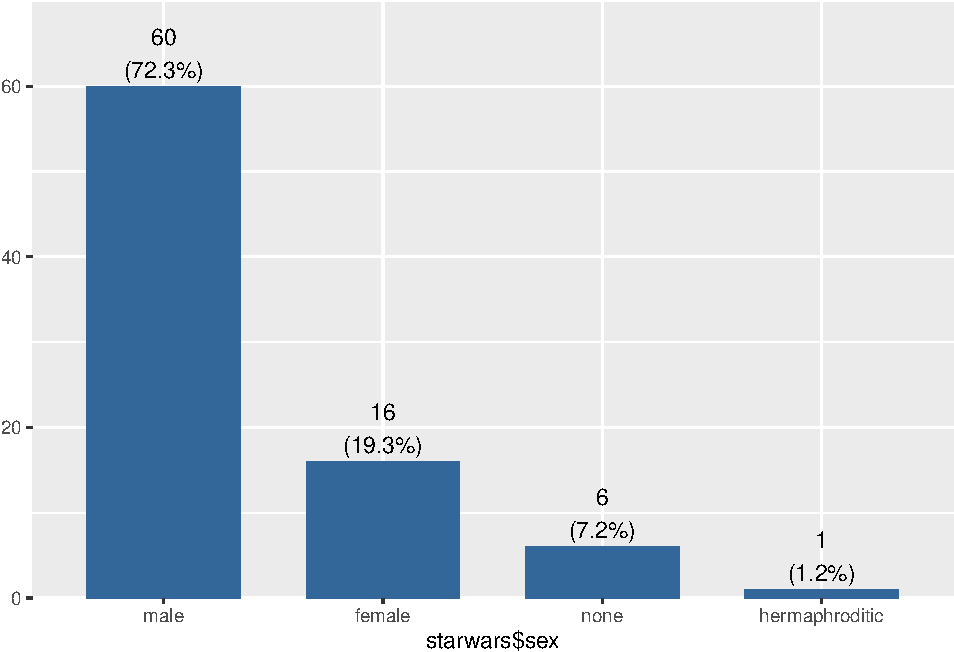
\includegraphics{r_book_files/figure-latex/freq_plot-1.pdf}

Über die Funktion \texttt{plot\_frq()} sind noch weitere Darstellungsformen möglich, wie bspw. ein Linien-Diagramm oder ein Diagramm mit Punkten. Man muss dazu lediglich das zusätzliche Argument \texttt{type} mit an die Funktion übergeben (z.B. \texttt{type\ =\ "line"} oder \texttt{type\ =\ "dot"}). Auch Histogramme sind möglich (\texttt{type\ =\ "histogram}), aber dazu später mehr.

\hypertarget{mauxdfe-der-zentralen-tendenz-streuung}{%
\section{Maße der zentralen Tendenz \& Streuung}\label{mauxdfe-der-zentralen-tendenz-streuung}}

Neben Häufigkeitsauszählungen dienen Maße der zentralen Tendenz und Streuung dazu, die Eigenschaften von Variablen sehr kompakt zu beschreiben. Ich ordne die Maßzahlen hier nach Datenniveau, beginnend bei niedrigsten bis zum höchsten. Selbstverständlich können Sie die Maße für ein niedrigeres Datenniveau auch für höhere Datenniveaus anwenden. Umgekehrt ist das jedoch nicht sinnvoll! Allerdings kennt R das Datenniveau der Variablen nicht. Es wird also ohne Probleme und Fehlermeldung auch ein arithmetisches Mittel für eine nominale Variable ausgeben. Das Denken kann uns R an dieser Stelle also leider nicht abnehmen. Wir müssen immer selbst vorab beurteilen, ob eine Berechnung sinnvoll ist oder nicht.

\hypertarget{nominale-daten}{%
\subsection{Nominale Daten}\label{nominale-daten}}

Als Beispiel für eine nominale Variable verwende ich die Frage, aus welchem Personenkreis die Vorbilder der Befragten kommen, sofern sie Vorbilder haben. Die Variable hat die folgenden Ausprägungen:

\begin{Shaded}
\begin{Highlighting}[]
\NormalTok{sjlabelled}\SpecialCharTok{::}\FunctionTok{get\_labels}\NormalTok{(data}\SpecialCharTok{$}\NormalTok{vorbild\_codiert)}
\end{Highlighting}
\end{Shaded}

\begin{verbatim}
## [1] "Eltern"                    "andere Familienangehörige"
## [3] "Musiker"                   "Sportler"                 
## [5] "religiöse Vorbilder"       "sonstige Promis"          
## [7] "Influencer"                "Sonstiges"                
## [9] "Weiß nicht"
\end{verbatim}

Der \textbf{Modus} ist der Wert in einer Verteilung, der am häufigsten vorkommt. Da die Reihenfolge der Ausprägungen dabei keine Rolle spielt, ist er sogar für nominale Daten anwendbar. Man kann ihn aber auch für ordinale und metrische Daten ermitteln.

Für den Modus gibt es in base-R keine Standard-Funktion, vielleicht ist er einfach zu simpel. Man kann den Modus einfach über eine Häufigkeitsauszählung ermitteln oder über ein Säulendiagram (siehe voriger Abschnitt).

Alternativ gibt es noch eine \texttt{Mode()}-Funktion im \texttt{DescTools}-Paket. Achtung! Das Paket ist etwas altmodisch bei der Benennung seiner Funktionen: \texttt{Mode()} muss hier zwingend groß geschrieben werden!!

\begin{Shaded}
\begin{Highlighting}[]
\FunctionTok{library}\NormalTok{(DescTools)}

\FunctionTok{Mode}\NormalTok{(data}\SpecialCharTok{$}\NormalTok{vorbild\_codiert, }\AttributeTok{na.rm =} \ConstantTok{TRUE}\NormalTok{)}
\end{Highlighting}
\end{Shaded}

\begin{verbatim}
## [1] 1
## attr(,"freq")
## [1] 136
\end{verbatim}

Die Funktion liefert gleich zwei Ergebnisse zurück: Zum einen den Wert, der die meisten Ausprägungen auf sich vereint, in diesem Fall die Ausprägung ``1'' (Modus = 1). Zum anderen die absolute Häufigkeit, die diese Ausprägung hat (n). Aus der Liste der Wertelabels oben wissen wir, dass es sich bei 1 um die ``Eltern'' handelt.

\hypertarget{ordinale-daten}{%
\subsection{Ordinale Daten}\label{ordinale-daten}}

Der \textbf{Median} teilt die (sortierten) Fälle einer Variablen in zwei gleich große Hälften. Er kann für ordinale und metrische Daten berechnet werden.

Die Funktion für den Median gibt es sogar in base-R. Sie heißt schlicht \texttt{median()}. Die Funktion benötigt zwei Argumente. Zum einen selbstverständlich den Verweis auf die Variable und zum anderen einen Hinweis, wie mit fehlenden Werten umgegangen werden soll. Da R nicht wissen kann, wie fehlende Werte einzuberechnen wären müssen sie vorab aus der Analyse entfernt werden, mit \texttt{na.rm\ =\ TRUE} (\emph{NA remove}).

\begin{Shaded}
\begin{Highlighting}[]
\FunctionTok{median}\NormalTok{(data}\SpecialCharTok{$}\NormalTok{zufriedenheit\_leben, }\AttributeTok{na.rm =} \ConstantTok{TRUE}\NormalTok{)}
\end{Highlighting}
\end{Shaded}

\begin{verbatim}
## [1] 2
\end{verbatim}

Die \textbf{Spannweite} (\emph{range}) gibt an, zwischen welchen Ausprägungen sich eine Variable bewegt also den höchsten und den niedrigsten Wert.

\begin{Shaded}
\begin{Highlighting}[]
\FunctionTok{range}\NormalTok{(data}\SpecialCharTok{$}\NormalTok{zufriedenheit\_leben, }\AttributeTok{na.rm =} \ConstantTok{TRUE}\NormalTok{)}
\end{Highlighting}
\end{Shaded}

\begin{verbatim}
## [1] 1 4
\end{verbatim}

Über die Funktionen \texttt{min()} und \texttt{max()} kann man sich übrigens auch einzeln das Minimum bzw. Maximum ausgeben lassen.

Wie oben erwähnt teilt der Median die Verteilung der Werte in zwei gleiche Hälften. Wenn man jedoch nicht zwei Hälften haben möchte sondern sich eher für Drittel, Viertel oder Fünftel interessiert, sind \textbf{Quantile} das Mittel der Wahl. Üblich sind eigentlich nur Quartile, also die Einteilung in Viertel. Deshalb gibt die base-R-Funktion \texttt{quantile()} standardmäßig die Grenzen der Quartile zurück.

\begin{Shaded}
\begin{Highlighting}[]
\FunctionTok{quantile}\NormalTok{(data}\SpecialCharTok{$}\NormalTok{alter, }\AttributeTok{na.rm =} \ConstantTok{TRUE}\NormalTok{)}
\end{Highlighting}
\end{Shaded}

\begin{verbatim}
##   0%  25%  50%  75% 100% 
##   14   16   19   22   24
\end{verbatim}

Es handelt sich um 5 Grenzen, weil der niedrigste und der hächste Wert mit ausgegeben werden. Die Quartile befinden sich quasi ``zwischen'' diesen 5 Grenzpunkten.

Der **Interquartil-Abstand* gibt den Abstand zwischen dem Ende des ersten und dem Beginn des letzten Quartils an, Also in unserem Beispiel den Abstand zwischen den Ausprägungen 16 und 22 Jahre (= 6 Jahre).

\begin{Shaded}
\begin{Highlighting}[]
\FunctionTok{IQR}\NormalTok{(data}\SpecialCharTok{$}\NormalTok{alter, }\AttributeTok{na.rm =} \ConstantTok{TRUE}\NormalTok{)}
\end{Highlighting}
\end{Shaded}

\begin{verbatim}
## [1] 6
\end{verbatim}

\hypertarget{metrische-daten}{%
\subsection{Metrische Daten}\label{metrische-daten}}

Für metrische Variablen können haben Sie die Auswahl zwischen allen hier vorgestellten Maßen der zentralen Tendenz. Üblich ist aber vor allem das \textbf{``arithmetische Mittel''}, umgangssprachlich oft auch als Durchschnitt oder Mittelwert bezeichnet. Die Funktion \texttt{mean()} habe ich in den Einführungskapiteln bereits als Beispiel genutzt.

\begin{Shaded}
\begin{Highlighting}[]
\FunctionTok{mean}\NormalTok{(data}\SpecialCharTok{$}\NormalTok{alter, }\AttributeTok{na.rm =} \ConstantTok{TRUE}\NormalTok{)}
\end{Highlighting}
\end{Shaded}

\begin{verbatim}
## [1] 19.12823
\end{verbatim}

Der Altersdurchschnitt im Sample beträgt also 19,1 Jahre.

Bei dieser Variable ist es nicht sinnvoll, aber mit \texttt{mean()} kann man sich auch ein \textbf{getrimmtes Mittel} ausgeben lassen, bei dem die oberen uns niedrigen X Prozent der Daten entfernt werden. So kann das arithmetische Mittel robust gemacht werden gegen Extremwerte (die es in dieser Variable nicht gibt).

\begin{Shaded}
\begin{Highlighting}[]
\FunctionTok{mean}\NormalTok{(data}\SpecialCharTok{$}\NormalTok{alter, }\AttributeTok{trim =} \FloatTok{0.1}\NormalTok{, }\AttributeTok{na.rm =} \ConstantTok{TRUE}\NormalTok{)}
\end{Highlighting}
\end{Shaded}

\begin{verbatim}
## [1] 19.15261
\end{verbatim}

Es macht Sinn, sich bei einer Variable nie allein das arithmetische Mittel anzusehen. Sie wüssten dann z.B. nicht ob ein Wert (z.B. 19 Jahre) nur erreicht wird, weil alle . Wie der Name schon sagt, geben \textbf{Streuungsmaße} Auskunft darüber, wie die Werte einer Variablen um den Mittelwert streuen oder variieren. Das wichtigste Streuungsmaß, welches auch immer gemeinsam mit dem arithmetischen Mittel angesehen und berichtet werden sollte ist die \textbf{Streuung} (\emph{standard deviation}).

\begin{Shaded}
\begin{Highlighting}[]
\FunctionTok{sd}\NormalTok{(data}\SpecialCharTok{$}\NormalTok{alter, }\AttributeTok{na.rm =} \ConstantTok{TRUE}\NormalTok{)}
\end{Highlighting}
\end{Shaded}

\begin{verbatim}
## [1] 3.177417
\end{verbatim}

Die Streuung ist bekanntlich die Wurzel der Varianz und als Streuungsmaß auch um einiges üblicher. Dennoch soll hier natürlich auch die Funktion für die Varianz nicht fehlen:

\begin{Shaded}
\begin{Highlighting}[]
\FunctionTok{var}\NormalTok{(data}\SpecialCharTok{$}\NormalTok{alter, }\AttributeTok{na.rm =} \ConstantTok{TRUE}\NormalTok{)}
\end{Highlighting}
\end{Shaded}

\begin{verbatim}
## [1] 10.09598
\end{verbatim}

\hypertarget{schiefe-und-kurtosis}{%
\section{Schiefe und Kurtosis}\label{schiefe-und-kurtosis}}

Weitere Kennwerte für die Form von Verteilungen sind die \textbf{Schiefe} (\emph{skew}) und \textbf{Kurtosis} (\emph{kurtosis}). Die Schiefe ist quasi das Gegenteil von Symmetrie. Kurtosis drückt aus wie spitz (nach oben gewölbt) oder flach eine Verteilung ist.

Im \texttt{psych}-Paket gibt es Funktionen für beides:

\begin{Shaded}
\begin{Highlighting}[]
\NormalTok{psych}\SpecialCharTok{::}\FunctionTok{skew}\NormalTok{(data}\SpecialCharTok{$}\NormalTok{alter, }\AttributeTok{na.rm =} \ConstantTok{TRUE}\NormalTok{)}
\end{Highlighting}
\end{Shaded}

\begin{verbatim}
## [1] -0.06328724
\end{verbatim}

Zur Erinnerung:

\begin{itemize}
\item
  Ist die Schiefe \textgreater{} 0 so ist die Verteilung rechtsschief (Modus \textless{} Median \textless{} arithmetisches Mittel).
\item
  Ist die Schiefe = 0, so ist die Verteilung symetrisch (Modus = Median = arithmetisches Mittel).
\item
  Ist die Schiefe \textless{} 0 so ist die Verteilung linksschief (Modus \textgreater{} Median \textgreater{} arithmetisches Mittel).
\end{itemize}

Die Verteilung des Alters im obigen Beispiel ist also nahezu symmetrisch, ein wenig linksschief.

Hier noch der Code zur Berechnung der Kurtosis:

\begin{Shaded}
\begin{Highlighting}[]
\NormalTok{psych}\SpecialCharTok{::}\FunctionTok{kurtosi}\NormalTok{(data}\SpecialCharTok{$}\NormalTok{alter, }\AttributeTok{na.rm =} \ConstantTok{TRUE}\NormalTok{)}
\end{Highlighting}
\end{Shaded}

\begin{verbatim}
## [1] -1.250003
\end{verbatim}

\hypertarget{uxfcbersichts-funktionen}{%
\section{Übersichts-Funktionen}\label{uxfcbersichts-funktionen}}

Bisher haben wir uns die Statistiken jeweils für eine einzelne Variable ausgeben lassen. Aber natürlich macht es Sinn, sich mehrere Kennwerte gleichzeitig ausgeben zu lassen. Die Funktion \texttt{summary()} aus dem base-Paket liefert zum Beispiel einen ersten guten Einblick:

\begin{Shaded}
\begin{Highlighting}[]
\FunctionTok{summary}\NormalTok{(data}\SpecialCharTok{$}\NormalTok{alter)}
\end{Highlighting}
\end{Shaded}

\begin{verbatim}
##    Min. 1st Qu.  Median    Mean 3rd Qu.    Max. 
##   14.00   16.00   19.00   19.13   22.00   24.00
\end{verbatim}

Allerdings fehlen an dieser Stelle z.B. die Streuungsmaße. Es geht also noch mehr. Das vorhin genutzte \texttt{psych}-Paket hat z.B. eine \texttt{describe()}-Funktion, mit der man sich gleichzeitig verschiedene deskriptive Statistiken ausgeben kann - und zwar nicht nur für eine Variable, sondern gleich für mehrere oder sogar für einen ganzen Datensatz.

\begin{Shaded}
\begin{Highlighting}[]
\NormalTok{psych}\SpecialCharTok{::}\FunctionTok{describe}\NormalTok{(data)}
\end{Highlighting}
\end{Shaded}

\begin{verbatim}
##                                                   vars    n    mean     sd
## za_nr                                                1 1006 6738.00   0.00
## version*                                             2 1006     NaN     NA
## doi*                                                 3 1006     NaN     NA
## lfdn                                                 4 1006 2314.19 407.58
## zufriedenheit_leben                                  5  996    1.94   0.61
## zukunftsperspektive_persoenlich                      6  985    1.92   0.61
## zukunftsperspektive_generation                       7  984    2.46   0.71
## eltern_verhaeltnis                                   8 1004    1.53   0.72
## eltern_unterstuetzung                                9  999    1.62   0.80
## eltern_ratgeber                                     10  997    2.06   0.86
## eltern_diskutieren                                  11  996    2.33   0.95
## eltern_zuhoerer                                     12  996    1.79   0.82
## bildung_vater                                       13  911    2.08   0.77
## bildung_mutter                                      14  947    2.07   0.71
## finanz_verzicht                                     15  998    2.27   0.84
## geld_eigene_arbeit                                  16 1006    0.64   0.48
## geld_eltern                                         17 1006    0.54   0.50
## geld_staat                                          18 1006    0.15   0.35
## geld_sonstige                                       19 1006    0.09   0.28
## geld_weiss_nicht                                    20 1006    0.00   0.06
## geld_hauptsaechlich                                 21  997    1.62   0.74
## vorbild_ja                                          22  793    1.50   0.50
## vorbild_welches                                     23  338    1.00   0.00
## vorbild_codiert                                     24  334    3.43   2.77
## fokus_leben_individualitaet                         25 1006    0.27   0.44
## fokus_leben_freiheit                                26 1006    0.42   0.49
## fokus_leben_hedonismus                              27 1006    0.53   0.50
## fokus_leben_karriere                                28 1006    0.21   0.41
## fokus_leben_altruismus                              29 1006    0.35   0.48
## fokus_leben_verantwortung                           30 1006    0.21   0.41
## fokus_leben_durchsetzung                            31 1006    0.07   0.26
## fokus_leben_toleranz                                32 1006    0.15   0.35
## fokus_leben_gesundheit                              33 1006    0.21   0.41
## fokus_leben_umwelt                                  34 1006    0.24   0.43
## fokus_leben_finanzen                                35 1006    0.59   0.49
## fokus_leben_luxus                                   36 1006    0.30   0.46
## fokus_leben_respekt                                 37 1006    0.16   0.37
## fokus_leben_unangepasstheit                         38 1006    0.10   0.30
## fokus_leben_vernatwortungsvoller_konsum             39 1006    0.09   0.29
## fokus_leben_kein                                    40 1006    0.00   0.04
## fokus_beruf_sicherheit                              41  998    1.64   0.77
## fokus_beruf_einkommen                               42 1005    1.71   0.74
## fokus_beruf_interesse                               43 1005    1.51   0.70
## fokus_beruf_work_life_balance                       44  990    1.80   0.85
## fokus_beruf_karriere                                45  992    2.38   0.96
## fokus_beruf_verantwortung                           46  991    2.32   0.92
## fokus_beruf_entwicklung                             47  994    2.09   0.88
## werte_sicherheit_vs_privatsphaere                   48  973    3.85   1.81
## werte_sm_provatsphaere_vs_sm_socialising            49  990    4.38   1.72
## werte_moeglichkeiten_vs_ueberforderung              50  983    2.99   1.65
## werte_gesundheit_vs_spass                           51  993    3.74   1.74
## werte_individualitaet_vs_sozialitaet                52  989    4.06   1.86
## werte_nachhaltigkeit_vs_konsum                      53  990    3.93   1.80
## werte_leistung_vs_solidaritaet                      54  957    4.37   1.80
## werte_chancengleichheit_vs_elite                    55  972    2.67   1.75
## werte_zukunft_vs_vergangenheit                      56  986    3.09   1.91
## werte_gleichstellungspolitik                        57  977    4.41   2.07
## verbundenheit_stadt                                 58  986    2.38   0.84
## verbundenheit_region                                59  978    2.34   0.84
## verbundenheit_bundesland                            60  971    2.39   0.88
## verbundenheit_deutschland                           61  974    2.08   0.82
## verbundenheit_europa                                62  951    2.28   0.90
## sm_nutzung                                          63 1005    2.09   0.88
## sm_nutzung_rang_facebook                            64  997    1.37   1.65
## sm_nutzung_rang_instagram                           65  997    1.30   1.05
## sm_nutzung_rang_twitter                             66  997    0.76   1.74
## sm_nutzung_rang_youtube                             67  997    1.89   1.32
## sm_nutzung_rang_linked_in                           68  997    0.45   1.71
## sm_nutzung_rang_xing                                69  997    0.51   1.80
## sm_nutzung_rang_tumbler                             70  997    0.52   1.79
## sm_nutzung_rang_reddit                              71  997    0.46   1.76
## sm_nutzung_rang_snapchat                            72  997    1.63   1.89
## sm_nutzung_rang_tiktok                              73  997    0.69   2.03
## sm_nutzung_rang_twitch                              74  997    0.71   2.12
## sm_nutzung_socializing                              75  997    0.66   0.47
## sm_nutzung_tagesgeschehen                           76  997    0.53   0.50
## sm_nutzung_neue_kontakte                            77  997    0.22   0.41
## sm_nutzung_organisation                             78  997    0.42   0.49
## sm_nutzung_promies                                  79  997    0.40   0.49
## sm_nutzung_marken                                   80  997    0.26   0.44
## sm_nutzung_zeitvertreib                             81  997    0.84   0.37
## sm_nutzung_bildung                                  82  588    0.39   0.49
## sm_nutzung_weiss_nicht                              83  997    0.01   0.07
## politisches_interesse                               84  999    2.57   0.87
## touchpoints_politik_arbeit_schule_uni               85  997    2.20   0.86
## touchpoints_politik_freunde_familie                 86 1003    2.27   0.80
## touchpoints_politik_soziale_netzwerke               87 1000    2.24   0.88
## touchpoints_politik_freizeit                        88  986    2.98   0.88
## touchpoints_politik_oeffentlicher_raum              89  994    2.71   0.85
## touchpoints_politik_medien                          90  998    1.96   0.85
## mediennutzung_politik                               91  992    2.99   1.24
## infoquelle_tv_nachrichten                           92  893    0.40   0.49
## infoquelle_talkshows                                93  893    0.07   0.26
## infoquelle_websites_institutionen_behoerden         94  893    0.08   0.27
## infoquelle_tv_satiere                               95  893    0.16   0.37
## infoquelle_print                                    96  893    0.18   0.39
## infoquelle_internet_nachrichten                     97  893    0.35   0.48
## infoquelle_radio_podcast                            98  893    0.24   0.43
## infoquelle_nachrichten_app                          99  893    0.25   0.43
## infoquelle_politik_blog                            100  893    0.02   0.13
## infoquelle_newsletter_messanger_abo                101  893    0.03   0.18
## infoquelle_google                                  102  893    0.36   0.48
## infoquelle_instagram                               103  893    0.15   0.36
## infoquelle_youtube                                 104  893    0.26   0.44
## infoquelle_twitter                                 105  893    0.05   0.22
## infoquelle_facebook                                106  893    0.19   0.40
## infoquelle_snapchat                                107  893    0.04   0.19
## infoquelle_sonstige_offen                          108  893    0.02   0.14
## vertrauen_medien_tv_nachrichten                    109  353    2.07   0.69
## vertrauen_medien_talkshows                         110   60    2.12   0.76
## vertrauen_medien_websites_institutionen_behoerden  111   68    1.93   0.78
## vertrauen_medien_tv_satiere                        112  141    2.01   0.77
## vertrauen_medien_print                             113  160    1.93   0.73
## vertrauen_medien_internet_nachrichten              114  306    2.04   0.67
## vertrauen_medien_radio_podcast                     115  211    2.03   0.66
## vertrauen_medien_nachrichten_app                   116  217    1.72   0.73
## vertrauen_medien_politik_blog                      117   15    2.40   0.63
## vertrauen_medien_newsletter_messanger_abo          118   31    2.23   0.67
## vertrauen_medien_google                            119  308    2.29   0.72
## vertrauen_medien_instagram                         120  132    2.47   0.71
## vertrauen_medien_youtube                           121  229    2.28   0.72
## vertrauen_medien_twitter                           122   47    2.26   0.67
## vertrauen_medien_facebook                          123  169    2.62   0.77
## vertrauen_medien_snapchat                          124   33    2.85   0.71
## vertrauen_medien_sonstige_offen                    125   13    2.00   0.91
## politik_demokratie_zufriedenheit                   126  945    2.57   0.78
## politik_demokratie_idee                            127  918    1.12   0.32
## politik_reformbedarf                               128  924    1.87   0.60
## politik_regierungszufriedenheit                    129  943    2.80   0.74
## vertrauen_institutionen_justiz                     130  957    2.30   0.83
## vertrauen_institutionen_ngos                       131  917    2.43   0.91
## vertrauen_institutionen_vereine                    132  882    2.55   0.79
## vertrauen_institutionen_bundesregierung            133  935    2.77   0.80
## vertrauen_institutionen_parteien                   134  922    2.98   0.71
## vertrauen_institutionen_bundestag                  135  914    2.77   0.81
## vertrauen_institutionen_polizei                    136  987    2.12   0.81
## vertrauen_institutionen_kirchen                    137  929    3.31   0.84
## vertrauen_institutionen_schule_uni                 138  965    2.28   0.75
## parteisympathie                                    139  685    5.64   2.33
## einstellung_politiker_nehmen_sorgen_ernst          140  964    3.13   0.76
## einstellung_politiker_verstaendlich                141  970    2.45   0.90
## einstellung_politiker_kommunikationskanaele        142  932    2.19   0.88
## einstellung_talkshows_junge_menchen                143  823    2.94   0.71
## einstellung_entscheidungsprozess_undurchsichtig    144  954    2.21   0.80
## einstellung_politik_wichtige_probleme              145  965    3.08   0.76
## einstellung_politik_einflussmoeglichkeit           146  962    2.84   0.82
## einstellung_keine_ueberzeugende_partei             147  923    2.37   0.93
## einstellung_politik_lebensfern                     148  953    2.94   0.94
## einstellung_politik_wirtschaftsinteressen          149  924    1.86   0.77
## einstellung_widerspruch_klima_kapitalismus         150  828    2.34   0.88
## einstellung_parteien_macht                         151  944    1.93   0.80
## germany_first                                      152  926    2.27   0.85
## meinung_eu_vorteile_deutschlend                    153  855    2.11   0.88
## meinung_eu_wohlstand                               154  880    2.09   0.82
## meinung_eu_anti_souveraenitaet                     155  882    2.54   0.90
## meinung_eu_gute_idee_schlechte_umsetzung           156  893    2.10   0.77
## meinung_eu_problemloesungsebene                    157  875    2.11   0.85
## pol_partizipation_wahl                             158  650    0.70   0.46
## pol_partizipation_petition                         159 1006    0.32   0.47
## pol_partizipation_sm_kommentar                     160 1006    0.15   0.36
## pol_partizipation_partei_veranstaltung             161 1006    0.08   0.28
## pol_partizipation_demo                             162 1006    0.13   0.33
## pol_partizipation_information                      163 1006    0.58   0.49
## pol_partizipation_gespraech                        164 1006    0.63   0.48
## pol_partizipation_produktboykott                   165 1006    0.26   0.44
## pol_partizipation_parteiengagement                 166 1006    0.04   0.19
## pol_partizipation_anderes_engagement               167 1006    0.05   0.21
## pol_partizipation_nichts_davon                     168 1006    0.18   0.39
## ehrenamt_allgemein                                 169  968    1.74   0.44
## ehrenamt_spezifisch                                170  235    1.00   0.00
## ehrenamt_codiert                                   171  234    4.07   2.76
## fff_interesse                                      172  981    2.46   1.00
## fff_teilnahme                                      173  991    4.36   0.92
## reaktionen_fff_agendasetting                       174  963    1.86   0.81
## reaktionen_fff_berichterstattung_positiv           175  859    2.44   0.75
## reaktionen_fff_mangelnde_berichterstattung         176  916    2.60   0.99
## reaktionen_fff_politiker_untaetigkeit              177  877    1.85   0.78
## reaktionen_fff_schulzeit_aufmerksamkeit            178  946    2.21   1.10
## reaktionen_fff_schulstreik_ungeeignet              179  949    2.58   1.08
## reaktionen_fff_teilnehmer_schwaenzen               180  923    2.58   1.03
## reaktionen_fff_konsumverzicht                      181  963    2.70   0.99
## reaktionen_fff_elternunterstuetzung                182  118    1.86   0.82
## alter                                              183 1006   19.13   3.18
## geschlecht                                         184 1006    1.48   0.50
## bundesland                                         185 1006    7.09   3.41
## bildung_derzeit                                    186 1006    1.41   0.49
## bildung_schule                                     187  593    3.57   1.16
## bildung_abschluss                                  188  527    3.27   0.98
## erwerbstaetigkeit                                  189  387    2.22   2.01
## wohnsituation                                      190  986    1.33   0.47
## gemeindegroesse                                    191  932    3.34   1.75
## migrationshintergrund                              192  993    3.69   0.68
## Gewicht                                            193 1006    1.00   0.18
## filter_$                                           194 1006    0.89   0.32
##                                                    median trimmed    mad
## za_nr                                             6738.00 6738.00   0.00
## version*                                               NA     NaN     NA
## doi*                                                   NA     NaN     NA
## lfdn                                              2309.00 2307.73 517.43
## zufriedenheit_leben                                  2.00    1.91   0.00
## zukunftsperspektive_persoenlich                      2.00    1.88   0.00
## zukunftsperspektive_generation                       2.00    2.45   1.48
## eltern_verhaeltnis                                   1.00    1.41   0.00
## eltern_unterstuetzung                                1.00    1.47   0.00
## eltern_ratgeber                                      2.00    1.98   1.48
## eltern_diskutieren                                   2.00    2.29   1.48
## eltern_zuhoerer                                      2.00    1.68   1.48
## bildung_vater                                        2.00    2.10   1.48
## bildung_mutter                                       2.00    2.09   1.48
## finanz_verzicht                                      2.00    2.24   1.48
## geld_eigene_arbeit                                   1.00    0.67   0.00
## geld_eltern                                          1.00    0.55   0.00
## geld_staat                                           0.00    0.06   0.00
## geld_sonstige                                        0.00    0.00   0.00
## geld_weiss_nicht                                     0.00    0.00   0.00
## geld_hauptsaechlich                                  1.00    1.50   0.00
## vorbild_ja                                           1.00    1.50   0.00
## vorbild_welches                                      1.00    1.00   0.00
## vorbild_codiert                                      2.00    3.04   1.48
## fokus_leben_individualitaet                          0.00    0.21   0.00
## fokus_leben_freiheit                                 0.00    0.40   0.00
## fokus_leben_hedonismus                               1.00    0.54   0.00
## fokus_leben_karriere                                 0.00    0.14   0.00
## fokus_leben_altruismus                               0.00    0.32   0.00
## fokus_leben_verantwortung                            0.00    0.13   0.00
## fokus_leben_durchsetzung                             0.00    0.00   0.00
## fokus_leben_toleranz                                 0.00    0.06   0.00
## fokus_leben_gesundheit                               0.00    0.13   0.00
## fokus_leben_umwelt                                   0.00    0.18   0.00
## fokus_leben_finanzen                                 1.00    0.61   0.00
## fokus_leben_luxus                                    0.00    0.25   0.00
## fokus_leben_respekt                                  0.00    0.08   0.00
## fokus_leben_unangepasstheit                          0.00    0.00   0.00
## fokus_leben_vernatwortungsvoller_konsum              0.00    0.00   0.00
## fokus_leben_kein                                     0.00    0.00   0.00
## fokus_beruf_sicherheit                               1.00    1.53   0.00
## fokus_beruf_einkommen                                2.00    1.62   1.48
## fokus_beruf_interesse                                1.00    1.39   0.00
## fokus_beruf_work_life_balance                        2.00    1.70   1.48
## fokus_beruf_karriere                                 2.00    2.34   1.48
## fokus_beruf_verantwortung                            2.00    2.27   1.48
## fokus_beruf_entwicklung                              2.00    2.04   1.48
## werte_sicherheit_vs_privatsphaere                    4.00    3.82   1.48
## werte_sm_provatsphaere_vs_sm_socialising             5.00    4.45   1.48
## werte_moeglichkeiten_vs_ueberforderung               3.00    2.82   1.48
## werte_gesundheit_vs_spass                            4.00    3.72   1.48
## werte_individualitaet_vs_sozialitaet                 4.00    4.07   2.97
## werte_nachhaltigkeit_vs_konsum                       4.00    3.91   1.48
## werte_leistung_vs_solidaritaet                       4.00    4.43   2.97
## werte_chancengleichheit_vs_elite                     2.00    2.43   1.48
## werte_zukunft_vs_vergangenheit                       2.00    2.89   1.48
## werte_gleichstellungspolitik                         4.00    4.51   2.97
## verbundenheit_stadt                                  2.00    2.35   1.48
## verbundenheit_region                                 2.00    2.31   1.48
## verbundenheit_bundesland                             2.00    2.37   1.48
## verbundenheit_deutschland                            2.00    2.04   1.48
## verbundenheit_europa                                 2.00    2.23   1.48
## sm_nutzung                                           2.00    1.96   0.00
## sm_nutzung_rang_facebook                             1.00    1.12   1.48
## sm_nutzung_rang_instagram                            1.00    1.19   1.48
## sm_nutzung_rang_twitter                              0.00    0.30   0.00
## sm_nutzung_rang_youtube                              2.00    1.83   1.48
## sm_nutzung_rang_linked_in                            0.00    0.00   0.00
## sm_nutzung_rang_xing                                 0.00    0.00   0.00
## sm_nutzung_rang_tumbler                              0.00    0.00   0.00
## sm_nutzung_rang_reddit                               0.00    0.00   0.00
## sm_nutzung_rang_snapchat                             1.00    1.36   1.48
## sm_nutzung_rang_tiktok                               0.00    0.11   0.00
## sm_nutzung_rang_twitch                               0.00    0.09   0.00
## sm_nutzung_socializing                               1.00    0.70   0.00
## sm_nutzung_tagesgeschehen                            1.00    0.54   0.00
## sm_nutzung_neue_kontakte                             0.00    0.15   0.00
## sm_nutzung_organisation                              0.00    0.40   0.00
## sm_nutzung_promies                                   0.00    0.38   0.00
## sm_nutzung_marken                                    0.00    0.20   0.00
## sm_nutzung_zeitvertreib                              1.00    0.93   0.00
## sm_nutzung_bildung                                   0.00    0.36   0.00
## sm_nutzung_weiss_nicht                               0.00    0.00   0.00
## politisches_interesse                                3.00    2.59   1.48
## touchpoints_politik_arbeit_schule_uni                2.00    2.16   1.48
## touchpoints_politik_freunde_familie                  2.00    2.26   1.48
## touchpoints_politik_soziale_netzwerke                2.00    2.19   1.48
## touchpoints_politik_freizeit                         3.00    3.06   1.48
## touchpoints_politik_oeffentlicher_raum               3.00    2.73   1.48
## touchpoints_politik_medien                           2.00    1.89   1.48
## mediennutzung_politik                                3.00    2.98   1.48
## infoquelle_tv_nachrichten                            0.00    0.37   0.00
## infoquelle_talkshows                                 0.00    0.00   0.00
## infoquelle_websites_institutionen_behoerden          0.00    0.00   0.00
## infoquelle_tv_satiere                                0.00    0.08   0.00
## infoquelle_print                                     0.00    0.10   0.00
## infoquelle_internet_nachrichten                      0.00    0.31   0.00
## infoquelle_radio_podcast                             0.00    0.17   0.00
## infoquelle_nachrichten_app                           0.00    0.18   0.00
## infoquelle_politik_blog                              0.00    0.00   0.00
## infoquelle_newsletter_messanger_abo                  0.00    0.00   0.00
## infoquelle_google                                    0.00    0.32   0.00
## infoquelle_instagram                                 0.00    0.07   0.00
## infoquelle_youtube                                   0.00    0.21   0.00
## infoquelle_twitter                                   0.00    0.00   0.00
## infoquelle_facebook                                  0.00    0.12   0.00
## infoquelle_snapchat                                  0.00    0.00   0.00
## infoquelle_sonstige_offen                            0.00    0.00   0.00
## vertrauen_medien_tv_nachrichten                      2.00    2.06   0.00
## vertrauen_medien_talkshows                           2.00    2.08   0.00
## vertrauen_medien_websites_institutionen_behoerden    2.00    1.86   0.00
## vertrauen_medien_tv_satiere                          2.00    1.97   1.48
## vertrauen_medien_print                               2.00    1.88   0.00
## vertrauen_medien_internet_nachrichten                2.00    2.04   0.00
## vertrauen_medien_radio_podcast                       2.00    2.02   0.00
## vertrauen_medien_nachrichten_app                     2.00    1.63   1.48
## vertrauen_medien_politik_blog                        2.00    2.46   1.48
## vertrauen_medien_newsletter_messanger_abo            2.00    2.28   0.00
## vertrauen_medien_google                              2.00    2.33   1.48
## vertrauen_medien_instagram                           3.00    2.55   0.00
## vertrauen_medien_youtube                             2.00    2.32   1.48
## vertrauen_medien_twitter                             2.00    2.31   1.48
## vertrauen_medien_facebook                            3.00    2.64   0.00
## vertrauen_medien_snapchat                            3.00    2.81   1.48
## vertrauen_medien_sonstige_offen                      2.00    1.91   1.48
## politik_demokratie_zufriedenheit                     2.00    2.53   1.48
## politik_demokratie_idee                              1.00    1.03   0.00
## politik_reformbedarf                                 2.00    1.83   0.00
## politik_regierungszufriedenheit                      3.00    2.78   1.48
## vertrauen_institutionen_justiz                       2.00    2.28   1.48
## vertrauen_institutionen_ngos                         2.00    2.41   1.48
## vertrauen_institutionen_vereine                      3.00    2.53   1.48
## vertrauen_institutionen_bundesregierung              3.00    2.77   1.48
## vertrauen_institutionen_parteien                     3.00    3.00   0.00
## vertrauen_institutionen_bundestag                    3.00    2.78   1.48
## vertrauen_institutionen_polizei                      2.00    2.08   0.00
## vertrauen_institutionen_kirchen                      4.00    3.43   0.00
## vertrauen_institutionen_schule_uni                   2.00    2.27   0.00
## parteisympathie                                      7.00    5.85   1.48
## einstellung_politiker_nehmen_sorgen_ernst            3.00    3.21   0.00
## einstellung_politiker_verstaendlich                  2.00    2.43   1.48
## einstellung_politiker_kommunikationskanaele          2.00    2.13   1.48
## einstellung_talkshows_junge_menchen                  3.00    2.95   0.00
## einstellung_entscheidungsprozess_undurchsichtig      2.00    2.19   1.48
## einstellung_politik_wichtige_probleme                3.00    3.13   1.48
## einstellung_politik_einflussmoeglichkeit             3.00    2.88   1.48
## einstellung_keine_ueberzeugende_partei               2.00    2.34   1.48
## einstellung_politik_lebensfern                       3.00    3.04   1.48
## einstellung_politik_wirtschaftsinteressen            2.00    1.79   1.48
## einstellung_widerspruch_klima_kapitalismus           2.00    2.31   1.48
## einstellung_parteien_macht                           2.00    1.88   1.48
## germany_first                                        3.00    2.34   0.00
## meinung_eu_vorteile_deutschlend                      2.00    2.04   1.48
## meinung_eu_wohlstand                                 2.00    2.04   0.00
## meinung_eu_anti_souveraenitaet                       3.00    2.55   1.48
## meinung_eu_gute_idee_schlechte_umsetzung             2.00    2.08   0.00
## meinung_eu_problemloesungsebene                      2.00    2.06   1.48
## pol_partizipation_wahl                               1.00    0.74   0.00
## pol_partizipation_petition                           0.00    0.28   0.00
## pol_partizipation_sm_kommentar                       0.00    0.06   0.00
## pol_partizipation_partei_veranstaltung               0.00    0.00   0.00
## pol_partizipation_demo                               0.00    0.03   0.00
## pol_partizipation_information                        1.00    0.61   0.00
## pol_partizipation_gespraech                          1.00    0.66   0.00
## pol_partizipation_produktboykott                     0.00    0.20   0.00
## pol_partizipation_parteiengagement                   0.00    0.00   0.00
## pol_partizipation_anderes_engagement                 0.00    0.00   0.00
## pol_partizipation_nichts_davon                       0.00    0.11   0.00
## ehrenamt_allgemein                                   2.00    1.79   0.00
## ehrenamt_spezifisch                                  1.00    1.00   0.00
## ehrenamt_codiert                                     3.00    3.85   2.97
## fff_interesse                                        2.00    2.45   1.48
## fff_teilnahme                                        5.00    4.55   0.00
## reaktionen_fff_agendasetting                         2.00    1.78   1.48
## reaktionen_fff_berichterstattung_positiv             2.00    2.44   1.48
## reaktionen_fff_mangelnde_berichterstattung           3.00    2.62   1.48
## reaktionen_fff_politiker_untaetigkeit                2.00    1.77   1.48
## reaktionen_fff_schulzeit_aufmerksamkeit              2.00    2.14   1.48
## reaktionen_fff_schulstreik_ungeeignet                3.00    2.60   1.48
## reaktionen_fff_teilnehmer_schwaenzen                 3.00    2.60   1.48
## reaktionen_fff_konsumverzicht                        3.00    2.74   1.48
## reaktionen_fff_elternunterstuetzung                  2.00    1.75   1.48
## alter                                               19.00   19.15   4.45
## geschlecht                                           1.00    1.48   0.00
## bundesland                                           7.00    6.82   2.97
## bildung_derzeit                                      1.00    1.39   0.00
## bildung_schule                                       3.00    3.58   1.48
## bildung_abschluss                                    3.00    3.22   1.48
## erwerbstaetigkeit                                    1.00    1.79   0.00
## wohnsituation                                        1.00    1.29   0.00
## gemeindegroesse                                      3.00    3.30   2.97
## migrationshintergrund                                4.00    3.88   0.00
## Gewicht                                              0.99    0.99   0.15
## filter_$                                             1.00    0.98   0.00
##                                                       min     max   range  skew
## za_nr                                             6738.00 6738.00    0.00   NaN
## version*                                              Inf    -Inf    -Inf    NA
## doi*                                                  Inf    -Inf    -Inf    NA
## lfdn                                              1634.00 3082.00 1448.00  0.09
## zufriedenheit_leben                                  1.00    4.00    3.00  0.27
## zukunftsperspektive_persoenlich                      1.00    4.00    3.00  0.49
## zukunftsperspektive_generation                       1.00    4.00    3.00  0.17
## eltern_verhaeltnis                                   1.00    4.00    3.00  1.40
## eltern_unterstuetzung                                1.00    4.00    3.00  1.31
## eltern_ratgeber                                      1.00    4.00    3.00  0.60
## eltern_diskutieren                                   1.00    4.00    3.00  0.23
## eltern_zuhoerer                                      1.00    4.00    3.00  0.92
## bildung_vater                                        1.00    3.00    2.00 -0.14
## bildung_mutter                                       1.00    3.00    2.00 -0.10
## finanz_verzicht                                      1.00    4.00    3.00  0.21
## geld_eigene_arbeit                                   0.00    1.00    1.00 -0.57
## geld_eltern                                          0.00    1.00    1.00 -0.15
## geld_staat                                           0.00    1.00    1.00  2.00
## geld_sonstige                                        0.00    1.00    1.00  2.92
## geld_weiss_nicht                                     0.00    1.00    1.00 15.74
## geld_hauptsaechlich                                  1.00    4.00    3.00  1.13
## vorbild_ja                                           1.00    2.00    1.00  0.01
## vorbild_welches                                      1.00    1.00    0.00   NaN
## vorbild_codiert                                      1.00    9.00    8.00  0.82
## fokus_leben_individualitaet                          0.00    1.00    1.00  1.06
## fokus_leben_freiheit                                 0.00    1.00    1.00  0.33
## fokus_leben_hedonismus                               0.00    1.00    1.00 -0.13
## fokus_leben_karriere                                 0.00    1.00    1.00  1.39
## fokus_leben_altruismus                               0.00    1.00    1.00  0.61
## fokus_leben_verantwortung                            0.00    1.00    1.00  1.45
## fokus_leben_durchsetzung                             0.00    1.00    1.00  3.23
## fokus_leben_toleranz                                 0.00    1.00    1.00  1.99
## fokus_leben_gesundheit                               0.00    1.00    1.00  1.45
## fokus_leben_umwelt                                   0.00    1.00    1.00  1.21
## fokus_leben_finanzen                                 0.00    1.00    1.00 -0.36
## fokus_leben_luxus                                    0.00    1.00    1.00  0.86
## fokus_leben_respekt                                  0.00    1.00    1.00  1.82
## fokus_leben_unangepasstheit                          0.00    1.00    1.00  2.66
## fokus_leben_vernatwortungsvoller_konsum              0.00    1.00    1.00  2.79
## fokus_leben_kein                                     0.00    1.00    1.00 22.33
## fokus_beruf_sicherheit                               1.00    5.00    4.00  0.98
## fokus_beruf_einkommen                                1.00    4.00    3.00  0.70
## fokus_beruf_interesse                                1.00    5.00    4.00  1.37
## fokus_beruf_work_life_balance                        1.00    5.00    4.00  0.90
## fokus_beruf_karriere                                 1.00    5.00    4.00  0.25
## fokus_beruf_verantwortung                            1.00    5.00    4.00  0.34
## fokus_beruf_entwicklung                              1.00    5.00    4.00  0.46
## werte_sicherheit_vs_privatsphaere                    1.00    7.00    6.00  0.18
## werte_sm_provatsphaere_vs_sm_socialising             1.00    7.00    6.00 -0.34
## werte_moeglichkeiten_vs_ueberforderung               1.00    7.00    6.00  0.65
## werte_gesundheit_vs_spass                            1.00    7.00    6.00  0.15
## werte_individualitaet_vs_sozialitaet                 1.00    7.00    6.00 -0.05
## werte_nachhaltigkeit_vs_konsum                       1.00    7.00    6.00  0.09
## werte_leistung_vs_solidaritaet                       1.00    7.00    6.00 -0.26
## werte_chancengleichheit_vs_elite                     1.00    7.00    6.00  0.89
## werte_zukunft_vs_vergangenheit                       1.00    7.00    6.00  0.68
## werte_gleichstellungspolitik                         1.00    7.00    6.00 -0.15
## verbundenheit_stadt                                  1.00    4.00    3.00  0.15
## verbundenheit_region                                 1.00    4.00    3.00  0.23
## verbundenheit_bundesland                             1.00    4.00    3.00  0.07
## verbundenheit_deutschland                            1.00    4.00    3.00  0.44
## verbundenheit_europa                                 1.00    4.00    3.00  0.22
## sm_nutzung                                           1.00    6.00    5.00  1.89
## sm_nutzung_rang_facebook                             0.00   11.00   11.00  1.60
## sm_nutzung_rang_instagram                            0.00    9.00    9.00  1.56
## sm_nutzung_rang_twitter                              0.00   11.00   11.00  2.38
## sm_nutzung_rang_youtube                              0.00    9.00    9.00  0.47
## sm_nutzung_rang_linked_in                            0.00   11.00   11.00  4.04
## sm_nutzung_rang_xing                                 0.00   11.00   11.00  3.74
## sm_nutzung_rang_tumbler                              0.00   11.00   11.00  3.58
## sm_nutzung_rang_reddit                               0.00   11.00   11.00  4.08
## sm_nutzung_rang_snapchat                             0.00   11.00   11.00  1.29
## sm_nutzung_rang_tiktok                               0.00   11.00   11.00  3.29
## sm_nutzung_rang_twitch                               0.00   11.00   11.00  3.30
## sm_nutzung_socializing                               0.00    1.00    1.00 -0.67
## sm_nutzung_tagesgeschehen                            0.00    1.00    1.00 -0.14
## sm_nutzung_neue_kontakte                             0.00    1.00    1.00  1.37
## sm_nutzung_organisation                              0.00    1.00    1.00  0.34
## sm_nutzung_promies                                   0.00    1.00    1.00  0.39
## sm_nutzung_marken                                    0.00    1.00    1.00  1.08
## sm_nutzung_zeitvertreib                              0.00    1.00    1.00 -1.87
## sm_nutzung_bildung                                   0.00    1.00    1.00  0.47
## sm_nutzung_weiss_nicht                               0.00    1.00    1.00 13.99
## politisches_interesse                                1.00    4.00    3.00 -0.14
## touchpoints_politik_arbeit_schule_uni                1.00    4.00    3.00  0.34
## touchpoints_politik_freunde_familie                  1.00    4.00    3.00  0.24
## touchpoints_politik_soziale_netzwerke                1.00    4.00    3.00  0.28
## touchpoints_politik_freizeit                         1.00    4.00    3.00 -0.49
## touchpoints_politik_oeffentlicher_raum               1.00    4.00    3.00 -0.18
## touchpoints_politik_medien                           1.00    4.00    3.00  0.55
## mediennutzung_politik                                1.00    5.00    4.00 -0.13
## infoquelle_tv_nachrichten                            0.00    1.00    1.00  0.41
## infoquelle_talkshows                                 0.00    1.00    1.00  3.35
## infoquelle_websites_institutionen_behoerden          0.00    1.00    1.00  3.16
## infoquelle_tv_satiere                                0.00    1.00    1.00  1.85
## infoquelle_print                                     0.00    1.00    1.00  1.65
## infoquelle_internet_nachrichten                      0.00    1.00    1.00  0.64
## infoquelle_radio_podcast                             0.00    1.00    1.00  1.23
## infoquelle_nachrichten_app                           0.00    1.00    1.00  1.18
## infoquelle_politik_blog                              0.00    1.00    1.00  7.51
## infoquelle_newsletter_messanger_abo                  0.00    1.00    1.00  5.08
## infoquelle_google                                    0.00    1.00    1.00  0.60
## infoquelle_instagram                                 0.00    1.00    1.00  1.92
## infoquelle_youtube                                   0.00    1.00    1.00  1.07
## infoquelle_twitter                                   0.00    1.00    1.00  4.00
## infoquelle_facebook                                  0.00    1.00    1.00  1.54
## infoquelle_snapchat                                  0.00    1.00    1.00  4.82
## infoquelle_sonstige_offen                            0.00    1.00    1.00  7.03
## vertrauen_medien_tv_nachrichten                      1.00    4.00    3.00  0.23
## vertrauen_medien_talkshows                           1.00    4.00    3.00  0.49
## vertrauen_medien_websites_institutionen_behoerden    1.00    4.00    3.00  0.68
## vertrauen_medien_tv_satiere                          1.00    4.00    3.00  0.36
## vertrauen_medien_print                               1.00    4.00    3.00  0.49
## vertrauen_medien_internet_nachrichten                1.00    4.00    3.00  0.15
## vertrauen_medien_radio_podcast                       1.00    4.00    3.00  0.26
## vertrauen_medien_nachrichten_app                     1.00    4.00    3.00  0.76
## vertrauen_medien_politik_blog                        1.00    3.00    2.00 -0.44
## vertrauen_medien_newsletter_messanger_abo            1.00    3.00    2.00 -0.26
## vertrauen_medien_google                              1.00    4.00    3.00 -0.13
## vertrauen_medien_instagram                           1.00    4.00    3.00 -0.46
## vertrauen_medien_youtube                             1.00    4.00    3.00 -0.06
## vertrauen_medien_twitter                             1.00    3.00    2.00 -0.33
## vertrauen_medien_facebook                            1.00    4.00    3.00 -0.33
## vertrauen_medien_snapchat                            2.00    4.00    2.00  0.21
## vertrauen_medien_sonstige_offen                      1.00    4.00    3.00  0.61
## politik_demokratie_zufriedenheit                     1.00    4.00    3.00  0.23
## politik_demokratie_idee                              1.00    2.00    1.00  2.34
## politik_reformbedarf                                 1.00    3.00    2.00  0.06
## politik_regierungszufriedenheit                      1.00    4.00    3.00  0.02
## vertrauen_institutionen_justiz                       1.00    4.00    3.00  0.19
## vertrauen_institutionen_ngos                         1.00    4.00    3.00  0.18
## vertrauen_institutionen_vereine                      1.00    4.00    3.00  0.10
## vertrauen_institutionen_bundesregierung              1.00    4.00    3.00 -0.12
## vertrauen_institutionen_parteien                     1.00    4.00    3.00 -0.31
## vertrauen_institutionen_bundestag                    1.00    4.00    3.00 -0.20
## vertrauen_institutionen_polizei                      1.00    4.00    3.00  0.41
## vertrauen_institutionen_kirchen                      1.00    4.00    3.00 -0.98
## vertrauen_institutionen_schule_uni                   1.00    4.00    3.00  0.29
## parteisympathie                                      1.00    9.00    8.00 -0.75
## einstellung_politiker_nehmen_sorgen_ernst            1.00    4.00    3.00 -0.70
## einstellung_politiker_verstaendlich                  1.00    4.00    3.00  0.13
## einstellung_politiker_kommunikationskanaele          1.00    4.00    3.00  0.36
## einstellung_talkshows_junge_menchen                  1.00    4.00    3.00 -0.33
## einstellung_entscheidungsprozess_undurchsichtig      1.00    4.00    3.00  0.28
## einstellung_politik_wichtige_probleme                1.00    4.00    3.00 -0.48
## einstellung_politik_einflussmoeglichkeit             1.00    4.00    3.00 -0.37
## einstellung_keine_ueberzeugende_partei               1.00    4.00    3.00  0.10
## einstellung_politik_lebensfern                       1.00    4.00    3.00 -0.55
## einstellung_politik_wirtschaftsinteressen            1.00    4.00    3.00  0.67
## einstellung_widerspruch_klima_kapitalismus           1.00    4.00    3.00  0.04
## einstellung_parteien_macht                           1.00    4.00    3.00  0.42
## germany_first                                        1.00    3.00    2.00 -0.55
## meinung_eu_vorteile_deutschlend                      1.00    4.00    3.00  0.45
## meinung_eu_wohlstand                                 1.00    4.00    3.00  0.51
## meinung_eu_anti_souveraenitaet                       1.00    4.00    3.00 -0.13
## meinung_eu_gute_idee_schlechte_umsetzung             1.00    4.00    3.00  0.32
## meinung_eu_problemloesungsebene                      1.00    4.00    3.00  0.40
## pol_partizipation_wahl                               0.00    1.00    1.00 -0.85
## pol_partizipation_petition                           0.00    1.00    1.00  0.76
## pol_partizipation_sm_kommentar                       0.00    1.00    1.00  1.98
## pol_partizipation_partei_veranstaltung               0.00    1.00    1.00  3.03
## pol_partizipation_demo                               0.00    1.00    1.00  2.25
## pol_partizipation_information                        0.00    1.00    1.00 -0.34
## pol_partizipation_gespraech                          0.00    1.00    1.00 -0.52
## pol_partizipation_produktboykott                     0.00    1.00    1.00  1.07
## pol_partizipation_parteiengagement                   0.00    1.00    1.00  4.99
## pol_partizipation_anderes_engagement                 0.00    1.00    1.00  4.29
## pol_partizipation_nichts_davon                       0.00    1.00    1.00  1.63
## ehrenamt_allgemein                                   1.00    2.00    1.00 -1.07
## ehrenamt_spezifisch                                  1.00    1.00    0.00   NaN
## ehrenamt_codiert                                     1.00    9.00    8.00  0.63
## fff_interesse                                        1.00    4.00    3.00  0.05
## fff_teilnahme                                        1.00    5.00    4.00 -1.57
## reaktionen_fff_agendasetting                         1.00    4.00    3.00  0.71
## reaktionen_fff_berichterstattung_positiv             1.00    4.00    3.00  0.11
## reaktionen_fff_mangelnde_berichterstattung           1.00    4.00    3.00 -0.17
## reaktionen_fff_politiker_untaetigkeit                1.00    4.00    3.00  0.77
## reaktionen_fff_schulzeit_aufmerksamkeit              1.00    4.00    3.00  0.37
## reaktionen_fff_schulstreik_ungeeignet                1.00    4.00    3.00 -0.11
## reaktionen_fff_teilnehmer_schwaenzen                 1.00    4.00    3.00 -0.11
## reaktionen_fff_konsumverzicht                        1.00    4.00    3.00 -0.18
## reaktionen_fff_elternunterstuetzung                  1.00    4.00    3.00  0.91
## alter                                               14.00   24.00   10.00 -0.06
## geschlecht                                           1.00    3.00    2.00  0.09
## bundesland                                           1.00   16.00   15.00  0.60
## bildung_derzeit                                      1.00    2.00    1.00  0.36
## bildung_schule                                       1.00    6.00    5.00  0.11
## bildung_abschluss                                    1.00    6.00    5.00  0.55
## erwerbstaetigkeit                                    1.00    7.00    6.00  1.57
## wohnsituation                                        1.00    2.00    1.00  0.71
## gemeindegroesse                                      1.00    6.00    5.00  0.18
## migrationshintergrund                                1.00    4.00    3.00 -2.13
## Gewicht                                              0.54    1.83    1.29  0.57
## filter_$                                             0.00    1.00    1.00 -2.45
##                                                   kurtosis    se
## za_nr                                                  NaN  0.00
## version*                                                NA    NA
## doi*                                                    NA    NA
## lfdn                                                 -1.17 12.85
## zufriedenheit_leben                                   0.52  0.02
## zukunftsperspektive_persoenlich                       1.30  0.02
## zukunftsperspektive_generation                       -0.22  0.02
## eltern_verhaeltnis                                    1.90  0.02
## eltern_unterstuetzung                                 1.32  0.03
## eltern_ratgeber                                      -0.19  0.03
## eltern_diskutieren                                   -0.85  0.03
## eltern_zuhoerer                                       0.33  0.03
## bildung_vater                                        -1.29  0.03
## bildung_mutter                                       -1.01  0.02
## finanz_verzicht                                      -0.57  0.03
## geld_eigene_arbeit                                   -1.68  0.02
## geld_eltern                                          -1.98  0.02
## geld_staat                                            2.00  0.01
## geld_sonstige                                         6.51  0.01
## geld_weiss_nicht                                    246.01  0.00
## geld_hauptsaechlich                                   1.04  0.02
## vorbild_ja                                           -2.00  0.02
## vorbild_welches                                        NaN  0.00
## vorbild_codiert                                      -0.69  0.15
## fokus_leben_individualitaet                          -0.88  0.01
## fokus_leben_freiheit                                 -1.89  0.02
## fokus_leben_hedonismus                               -1.99  0.02
## fokus_leben_karriere                                 -0.07  0.01
## fokus_leben_altruismus                               -1.62  0.02
## fokus_leben_verantwortung                             0.09  0.01
## fokus_leben_durchsetzung                              8.47  0.01
## fokus_leben_toleranz                                  1.96  0.01
## fokus_leben_gesundheit                                0.09  0.01
## fokus_leben_umwelt                                   -0.53  0.01
## fokus_leben_finanzen                                 -1.87  0.02
## fokus_leben_luxus                                    -1.27  0.01
## fokus_leben_respekt                                   1.32  0.01
## fokus_leben_unangepasstheit                           5.06  0.01
## fokus_leben_vernatwortungsvoller_konsum               5.79  0.01
## fokus_leben_kein                                    497.01  0.00
## fokus_beruf_sicherheit                                0.27  0.02
## fokus_beruf_einkommen                                -0.29  0.02
## fokus_beruf_interesse                                 1.90  0.02
## fokus_beruf_work_life_balance                         0.45  0.03
## fokus_beruf_karriere                                 -0.53  0.03
## fokus_beruf_verantwortung                            -0.20  0.03
## fokus_beruf_entwicklung                              -0.29  0.03
## werte_sicherheit_vs_privatsphaere                    -0.96  0.06
## werte_sm_provatsphaere_vs_sm_socialising             -0.77  0.05
## werte_moeglichkeiten_vs_ueberforderung               -0.48  0.05
## werte_gesundheit_vs_spass                            -0.94  0.06
## werte_individualitaet_vs_sozialitaet                 -1.22  0.06
## werte_nachhaltigkeit_vs_konsum                       -1.06  0.06
## werte_leistung_vs_solidaritaet                       -0.91  0.06
## werte_chancengleichheit_vs_elite                     -0.26  0.06
## werte_zukunft_vs_vergangenheit                       -0.72  0.06
## werte_gleichstellungspolitik                         -1.31  0.07
## verbundenheit_stadt                                  -0.55  0.03
## verbundenheit_region                                 -0.49  0.03
## verbundenheit_bundesland                             -0.71  0.03
## verbundenheit_deutschland                            -0.30  0.03
## verbundenheit_europa                                 -0.72  0.03
## sm_nutzung                                            5.02  0.03
## sm_nutzung_rang_facebook                              4.10  0.05
## sm_nutzung_rang_instagram                             6.42  0.03
## sm_nutzung_rang_twitter                               5.43  0.06
## sm_nutzung_rang_youtube                               0.35  0.04
## sm_nutzung_rang_linked_in                            16.45  0.05
## sm_nutzung_rang_xing                                 13.69  0.06
## sm_nutzung_rang_tumbler                              12.29  0.06
## sm_nutzung_rang_reddit                               16.03  0.06
## sm_nutzung_rang_snapchat                              2.37  0.06
## sm_nutzung_rang_tiktok                               10.80  0.06
## sm_nutzung_rang_twitch                               10.79  0.07
## sm_nutzung_socializing                               -1.55  0.02
## sm_nutzung_tagesgeschehen                            -1.98  0.02
## sm_nutzung_neue_kontakte                             -0.13  0.01
## sm_nutzung_organisation                              -1.89  0.02
## sm_nutzung_promies                                   -1.85  0.02
## sm_nutzung_marken                                    -0.83  0.01
## sm_nutzung_zeitvertreib                               1.49  0.01
## sm_nutzung_bildung                                   -1.79  0.02
## sm_nutzung_weiss_nicht                              194.01  0.00
## politisches_interesse                                -0.66  0.03
## touchpoints_politik_arbeit_schule_uni                -0.49  0.03
## touchpoints_politik_freunde_familie                  -0.39  0.03
## touchpoints_politik_soziale_netzwerke                -0.62  0.03
## touchpoints_politik_freizeit                         -0.57  0.03
## touchpoints_politik_oeffentlicher_raum               -0.59  0.03
## touchpoints_politik_medien                           -0.40  0.03
## mediennutzung_politik                                -1.10  0.04
## infoquelle_tv_nachrichten                            -1.84  0.02
## infoquelle_talkshows                                  9.22  0.01
## infoquelle_websites_institutionen_behoerden           8.00  0.01
## infoquelle_tv_satiere                                 1.43  0.01
## infoquelle_print                                      0.73  0.01
## infoquelle_internet_nachrichten                      -1.59  0.02
## infoquelle_radio_podcast                             -0.50  0.01
## infoquelle_nachrichten_app                           -0.60  0.01
## infoquelle_politik_blog                              54.42  0.00
## infoquelle_newsletter_messanger_abo                  23.78  0.01
## infoquelle_google                                    -1.64  0.02
## infoquelle_instagram                                  1.69  0.01
## infoquelle_youtube                                   -0.86  0.01
## infoquelle_twitter                                   14.02  0.01
## infoquelle_facebook                                   0.37  0.01
## infoquelle_snapchat                                  21.25  0.01
## infoquelle_sonstige_offen                            47.44  0.00
## vertrauen_medien_tv_nachrichten                      -0.08  0.04
## vertrauen_medien_talkshows                            0.09  0.10
## vertrauen_medien_websites_institutionen_behoerden     0.28  0.09
## vertrauen_medien_tv_satiere                          -0.37  0.06
## vertrauen_medien_print                                0.09  0.06
## vertrauen_medien_internet_nachrichten                -0.26  0.04
## vertrauen_medien_radio_podcast                        0.12  0.05
## vertrauen_medien_nachrichten_app                      0.18  0.05
## vertrauen_medien_politik_blog                        -0.95  0.16
## vertrauen_medien_newsletter_messanger_abo            -0.90  0.12
## vertrauen_medien_google                              -0.54  0.04
## vertrauen_medien_instagram                           -0.38  0.06
## vertrauen_medien_youtube                             -0.48  0.05
## vertrauen_medien_twitter                             -0.89  0.10
## vertrauen_medien_facebook                            -0.25  0.06
## vertrauen_medien_snapchat                            -1.09  0.12
## vertrauen_medien_sonstige_offen                      -0.56  0.25
## politik_demokratie_zufriedenheit                     -0.51  0.03
## politik_demokratie_idee                               3.47  0.01
## politik_reformbedarf                                 -0.35  0.02
## politik_regierungszufriedenheit                      -0.61  0.02
## vertrauen_institutionen_justiz                       -0.52  0.03
## vertrauen_institutionen_ngos                         -0.78  0.03
## vertrauen_institutionen_vereine                      -0.49  0.03
## vertrauen_institutionen_bundesregierung              -0.55  0.03
## vertrauen_institutionen_parteien                     -0.09  0.02
## vertrauen_institutionen_bundestag                    -0.48  0.03
## vertrauen_institutionen_polizei                      -0.23  0.03
## vertrauen_institutionen_kirchen                       0.05  0.03
## vertrauen_institutionen_schule_uni                   -0.15  0.02
## parteisympathie                                      -0.58  0.09
## einstellung_politiker_nehmen_sorgen_ernst             0.37  0.02
## einstellung_politiker_verstaendlich                  -0.75  0.03
## einstellung_politiker_kommunikationskanaele          -0.57  0.03
## einstellung_talkshows_junge_menchen                   0.04  0.02
## einstellung_entscheidungsprozess_undurchsichtig      -0.37  0.03
## einstellung_politik_wichtige_probleme                -0.19  0.02
## einstellung_politik_einflussmoeglichkeit             -0.34  0.03
## einstellung_keine_ueberzeugende_partei               -0.86  0.03
## einstellung_politik_lebensfern                       -0.62  0.03
## einstellung_politik_wirtschaftsinteressen             0.19  0.03
## einstellung_widerspruch_klima_kapitalismus           -0.78  0.03
## einstellung_parteien_macht                           -0.59  0.03
## germany_first                                        -1.38  0.03
## meinung_eu_vorteile_deutschlend                      -0.51  0.03
## meinung_eu_wohlstand                                 -0.13  0.03
## meinung_eu_anti_souveraenitaet                       -0.77  0.03
## meinung_eu_gute_idee_schlechte_umsetzung             -0.27  0.03
## meinung_eu_problemloesungsebene                      -0.48  0.03
## pol_partizipation_wahl                               -1.28  0.02
## pol_partizipation_petition                           -1.43  0.01
## pol_partizipation_sm_kommentar                        1.92  0.01
## pol_partizipation_partei_veranstaltung                7.19  0.01
## pol_partizipation_demo                                3.05  0.01
## pol_partizipation_information                        -1.88  0.02
## pol_partizipation_gespraech                          -1.73  0.02
## pol_partizipation_produktboykott                     -0.85  0.01
## pol_partizipation_parteiengagement                   22.93  0.01
## pol_partizipation_anderes_engagement                 16.41  0.01
## pol_partizipation_nichts_davon                        0.66  0.01
## ehrenamt_allgemein                                   -0.86  0.01
## ehrenamt_spezifisch                                    NaN  0.00
## ehrenamt_codiert                                     -0.97  0.18
## fff_interesse                                        -1.08  0.03
## fff_teilnahme                                         1.98  0.03
## reaktionen_fff_agendasetting                          0.00  0.03
## reaktionen_fff_berichterstattung_positiv             -0.31  0.03
## reaktionen_fff_mangelnde_berichterstattung           -1.01  0.03
## reaktionen_fff_politiker_untaetigkeit                 0.39  0.03
## reaktionen_fff_schulzeit_aufmerksamkeit              -1.22  0.04
## reaktionen_fff_schulstreik_ungeeignet                -1.25  0.03
## reaktionen_fff_teilnehmer_schwaenzen                 -1.14  0.03
## reaktionen_fff_konsumverzicht                        -1.03  0.03
## reaktionen_fff_elternunterstuetzung                   0.56  0.08
## alter                                                -1.25  0.10
## geschlecht                                           -1.93  0.02
## bundesland                                            0.06  0.11
## bildung_derzeit                                      -1.87  0.02
## bildung_schule                                       -0.66  0.05
## bildung_abschluss                                     0.86  0.04
## erwerbstaetigkeit                                     0.95  0.10
## wohnsituation                                        -1.49  0.02
## gemeindegroesse                                      -1.34  0.06
## migrationshintergrund                                 3.50  0.02
## Gewicht                                               1.33  0.01
## filter_$                                              4.02  0.01
\end{verbatim}

Da sind jetzt sogar einige dabei, die wir bisher gar nicht besprochen haben (und auch nicht besprechen werden). Über verschiedene Argumente kann man sich noch weitere Kennzahlen in der Tabelle anzeigen lassen (z.B. \texttt{skew\ =\ TRUE} oder \texttt{ranges\ =\ TRUE}). Allerdings fällt auch auf, dass die Berechnungen nicht für alle Variablen sinnvoll sind. Die Variable \texttt{lfdn} gibt z.B. einfach die ID des Befragten an. Ein Mittelwert der Befragtennummer ist keine nützliche Angabe. R rechnet alle Statistiken einfach aus, ganz unabhängig davon, ob dies zulässig ist!

  \bibliography{book.bib}

\end{document}
